\documentclass[11pt,a4paper]{article}

\usepackage[utf8]{inputenc}
\usepackage[T1]{fontenc}
\usepackage{babel}
\babelprovide[main,import]{spanish}
\usepackage[a4paper,margin=2.3cm]{geometry}
\usepackage{lmodern}
\usepackage{microtype}
\usepackage{amsmath,amssymb}
\usepackage{booktabs}
\usepackage{longtable}
\usepackage{array}
\usepackage{enumitem}
\usepackage{tabularx}
\usepackage{graphicx}
\usepackage{pdflscape}
\usepackage{tikz}
\usepackage{eso-pic}
\usepackage{xcolor}
\usepackage{hyperref}
\usepackage{fancyhdr}
\usepackage{lastpage}

\definecolor{azuluh}{HTML}{123B63}
\definecolor{gris}{HTML}{5B6573}

\hypersetup{colorlinks=true,linkcolor=azuluh,urlcolor=azuluh,pdftitle={Informe de diseño de la base de datos - Rutas de reparto},pdfauthor={Equipo Digimons}}
\setlength{\parindent}{0pt}
\setlength{\parskip}{6pt}
\renewcommand{\arraystretch}{1.25}
\setlist[itemize]{leftmargin=*,itemsep=2pt}
\setlist[enumerate]{leftmargin=*,itemsep=3pt}
\pagestyle{fancy}
\setlength{\headheight}{15pt}
\fancyhf{}
\lhead{Gestión de rutas de reparto de última milla}
\rhead{Informe de diseño de BD}
\cfoot{\thepage\ de \pageref{LastPage}}
\renewcommand{\headrulewidth}{0.4pt}

\newcolumntype{Y}{>{\raggedright\arraybackslash}X}
\newcolumntype{P}[1]{>{\raggedright\arraybackslash\let\_\ubrk}p{#1}}
\newcommand{\ubrk}{\textunderscore\allowbreak}
\newcommand{\campo}[1]{\textnormal{\ttfamily\let\_\ubrk #1}}
\newcommand{\pk}[1]{\underline{\texttt{#1}}}
\newcommand{\tabla}[1]{\begingroup\sffamily\bfseries\let\_\ubrk #1\endgroup}
\newcommand{\df}[3]{\item[$f_{#1}$:] \{#2\} $\rightarrow$ \{#3\}}
\newcommand{\trig}{\textit{(Disparador.)}}

\AddToShipoutPictureBG{%
  \begin{tikzpicture}[remember picture,overlay]
    \node[opacity=0.07] at (current page.center) {
\includegraphics[width=0.65\paperwidth]{MATCOM.png}};
  \end{tikzpicture}%
}

% generado por chase_latex.py
\newcommand{\leyendaU}{1~\campo{id\_coordinador}; 2~\campo{nombre\_coordinador}; 3~\campo{especialidad}; 4~\campo{id\_repartidor}; 5~\campo{nombre\_repartidor}; 6~\campo{edad}; 7~\campo{flota}; 8~\campo{id\_supervisor}; 9~\campo{nombre\_supervisor}; 10~\campo{area\_control}; 11~\campo{id\_centro}; 12~\campo{nombre\_centro}; 13~\campo{programa\_logistico}; 14~\campo{id\_zona}; 15~\campo{nombre\_zona}; 16~\campo{id\_parada}; 17~\campo{direccion}; 18~\campo{id\_pedido}; 19~\campo{descripcion}; 20~\campo{tipo\_entrega}; 21~\campo{prioridad}; 22~\campo{peso\_kg}; 23~\campo{fecha\_ingreso}; 24~\campo{fecha\_hora\_limite}; 25~\campo{estado\_pedido}; 26~\campo{id\_coord\_ingreso}; 27~\campo{id\_centro\_pedido}; 28~\campo{id\_criterio}; 29~\campo{nombre\_criterio}; 30~\campo{descripcion\_criterio}; 31~\campo{id\_coord\_autor}; 32~\campo{id\_parametro}; 33~\campo{nombre\_parametro}; 34~\campo{metrica}; 35~\campo{operador}; 36~\campo{tipo\_entrega\_objetivo}; 37~\campo{id\_ruta}; 38~\campo{fecha\_creacion}; 39~\campo{fecha\_programada}; 40~\campo{capacidad\_vehiculo\_kg}; 41~\campo{id\_coord\_generador}; 42~\campo{id\_centro\_ruta}; 43~\campo{id\_revision\_origen}; 44~\campo{id\_revision}; 45~\campo{fecha\_hora\_revision}; 46~\campo{decision}; 47~\campo{observaciones\_revision}; 48~\campo{id\_entrega}; 49~\campo{fecha\_hora\_entrega}; 50~\campo{resultado}; 51~\campo{observaciones\_entrega}; 52~\campo{id\_reprogramacion}; 53~\campo{fecha\_solicitud}; 54~\campo{motivo}; 55~\campo{estado\_solicitud}; 56~\campo{resultado\_manual}; 57~\campo{fecha\_resolucion}; 58~\campo{id\_coord\_resolutor}; 59~\campo{orden\_visita}; 60~\campo{valor\_aplicado}; 61~\campo{valor\_indicado}}
\newcommand{\matrizinicial}{\begin{tabular}{@{}l*{61}{@{\hspace{1.6pt}}c}@{}}
\toprule
 & 1 & 2 & 3 & 4 & 5 & 6 & 7 & 8 & 9 & 10 & 11 & 12 & 13 & 14 & 15 & 16 & 17 & 18 & 19 & 20 & 21 & 22 & 23 & 24 & 25 & 26 & 27 & 28 & 29 & 30 & 31 & 32 & 33 & 34 & 35 & 36 & 37 & 38 & 39 & 40 & 41 & 42 & 43 & 44 & 45 & 46 & 47 & 48 & 49 & 50 & 51 & 52 & 53 & 54 & 55 & 56 & 57 & 58 & 59 & 60 & 61\\ \midrule
COORDINADOR\_LOGISTICO & $a$ & $a$ & $a$ & \textcolor{gray}{$b$} & \textcolor{gray}{$b$} & \textcolor{gray}{$b$} & \textcolor{gray}{$b$} & \textcolor{gray}{$b$} & \textcolor{gray}{$b$} & \textcolor{gray}{$b$} & \textcolor{gray}{$b$} & \textcolor{gray}{$b$} & \textcolor{gray}{$b$} & \textcolor{gray}{$b$} & \textcolor{gray}{$b$} & \textcolor{gray}{$b$} & \textcolor{gray}{$b$} & \textcolor{gray}{$b$} & \textcolor{gray}{$b$} & \textcolor{gray}{$b$} & \textcolor{gray}{$b$} & \textcolor{gray}{$b$} & \textcolor{gray}{$b$} & \textcolor{gray}{$b$} & \textcolor{gray}{$b$} & \textcolor{gray}{$b$} & \textcolor{gray}{$b$} & \textcolor{gray}{$b$} & \textcolor{gray}{$b$} & \textcolor{gray}{$b$} & \textcolor{gray}{$b$} & \textcolor{gray}{$b$} & \textcolor{gray}{$b$} & \textcolor{gray}{$b$} & \textcolor{gray}{$b$} & \textcolor{gray}{$b$} & \textcolor{gray}{$b$} & \textcolor{gray}{$b$} & \textcolor{gray}{$b$} & \textcolor{gray}{$b$} & \textcolor{gray}{$b$} & \textcolor{gray}{$b$} & \textcolor{gray}{$b$} & \textcolor{gray}{$b$} & \textcolor{gray}{$b$} & \textcolor{gray}{$b$} & \textcolor{gray}{$b$} & \textcolor{gray}{$b$} & \textcolor{gray}{$b$} & \textcolor{gray}{$b$} & \textcolor{gray}{$b$} & \textcolor{gray}{$b$} & \textcolor{gray}{$b$} & \textcolor{gray}{$b$} & \textcolor{gray}{$b$} & \textcolor{gray}{$b$} & \textcolor{gray}{$b$} & \textcolor{gray}{$b$} & \textcolor{gray}{$b$} & \textcolor{gray}{$b$} & \textcolor{gray}{$b$}\\
REPARTIDOR & \textcolor{gray}{$b$} & \textcolor{gray}{$b$} & \textcolor{gray}{$b$} & $a$ & $a$ & $a$ & $a$ & \textcolor{gray}{$b$} & \textcolor{gray}{$b$} & \textcolor{gray}{$b$} & \textcolor{gray}{$b$} & \textcolor{gray}{$b$} & \textcolor{gray}{$b$} & \textcolor{gray}{$b$} & \textcolor{gray}{$b$} & \textcolor{gray}{$b$} & \textcolor{gray}{$b$} & \textcolor{gray}{$b$} & \textcolor{gray}{$b$} & \textcolor{gray}{$b$} & \textcolor{gray}{$b$} & \textcolor{gray}{$b$} & \textcolor{gray}{$b$} & \textcolor{gray}{$b$} & \textcolor{gray}{$b$} & \textcolor{gray}{$b$} & \textcolor{gray}{$b$} & \textcolor{gray}{$b$} & \textcolor{gray}{$b$} & \textcolor{gray}{$b$} & \textcolor{gray}{$b$} & \textcolor{gray}{$b$} & \textcolor{gray}{$b$} & \textcolor{gray}{$b$} & \textcolor{gray}{$b$} & \textcolor{gray}{$b$} & \textcolor{gray}{$b$} & \textcolor{gray}{$b$} & \textcolor{gray}{$b$} & \textcolor{gray}{$b$} & \textcolor{gray}{$b$} & \textcolor{gray}{$b$} & \textcolor{gray}{$b$} & \textcolor{gray}{$b$} & \textcolor{gray}{$b$} & \textcolor{gray}{$b$} & \textcolor{gray}{$b$} & \textcolor{gray}{$b$} & \textcolor{gray}{$b$} & \textcolor{gray}{$b$} & \textcolor{gray}{$b$} & \textcolor{gray}{$b$} & \textcolor{gray}{$b$} & \textcolor{gray}{$b$} & \textcolor{gray}{$b$} & \textcolor{gray}{$b$} & \textcolor{gray}{$b$} & \textcolor{gray}{$b$} & \textcolor{gray}{$b$} & \textcolor{gray}{$b$} & \textcolor{gray}{$b$}\\
SUPERVISOR\_OPERACIONES & \textcolor{gray}{$b$} & \textcolor{gray}{$b$} & \textcolor{gray}{$b$} & \textcolor{gray}{$b$} & \textcolor{gray}{$b$} & \textcolor{gray}{$b$} & \textcolor{gray}{$b$} & $a$ & $a$ & $a$ & \textcolor{gray}{$b$} & \textcolor{gray}{$b$} & \textcolor{gray}{$b$} & \textcolor{gray}{$b$} & \textcolor{gray}{$b$} & \textcolor{gray}{$b$} & \textcolor{gray}{$b$} & \textcolor{gray}{$b$} & \textcolor{gray}{$b$} & \textcolor{gray}{$b$} & \textcolor{gray}{$b$} & \textcolor{gray}{$b$} & \textcolor{gray}{$b$} & \textcolor{gray}{$b$} & \textcolor{gray}{$b$} & \textcolor{gray}{$b$} & \textcolor{gray}{$b$} & \textcolor{gray}{$b$} & \textcolor{gray}{$b$} & \textcolor{gray}{$b$} & \textcolor{gray}{$b$} & \textcolor{gray}{$b$} & \textcolor{gray}{$b$} & \textcolor{gray}{$b$} & \textcolor{gray}{$b$} & \textcolor{gray}{$b$} & \textcolor{gray}{$b$} & \textcolor{gray}{$b$} & \textcolor{gray}{$b$} & \textcolor{gray}{$b$} & \textcolor{gray}{$b$} & \textcolor{gray}{$b$} & \textcolor{gray}{$b$} & \textcolor{gray}{$b$} & \textcolor{gray}{$b$} & \textcolor{gray}{$b$} & \textcolor{gray}{$b$} & \textcolor{gray}{$b$} & \textcolor{gray}{$b$} & \textcolor{gray}{$b$} & \textcolor{gray}{$b$} & \textcolor{gray}{$b$} & \textcolor{gray}{$b$} & \textcolor{gray}{$b$} & \textcolor{gray}{$b$} & \textcolor{gray}{$b$} & \textcolor{gray}{$b$} & \textcolor{gray}{$b$} & \textcolor{gray}{$b$} & \textcolor{gray}{$b$} & \textcolor{gray}{$b$}\\
CENTRO\_DISTRIBUCION & \textcolor{gray}{$b$} & \textcolor{gray}{$b$} & \textcolor{gray}{$b$} & \textcolor{gray}{$b$} & \textcolor{gray}{$b$} & \textcolor{gray}{$b$} & \textcolor{gray}{$b$} & \textcolor{gray}{$b$} & \textcolor{gray}{$b$} & \textcolor{gray}{$b$} & $a$ & $a$ & $a$ & \textcolor{gray}{$b$} & \textcolor{gray}{$b$} & \textcolor{gray}{$b$} & \textcolor{gray}{$b$} & \textcolor{gray}{$b$} & \textcolor{gray}{$b$} & \textcolor{gray}{$b$} & \textcolor{gray}{$b$} & \textcolor{gray}{$b$} & \textcolor{gray}{$b$} & \textcolor{gray}{$b$} & \textcolor{gray}{$b$} & \textcolor{gray}{$b$} & \textcolor{gray}{$b$} & \textcolor{gray}{$b$} & \textcolor{gray}{$b$} & \textcolor{gray}{$b$} & \textcolor{gray}{$b$} & \textcolor{gray}{$b$} & \textcolor{gray}{$b$} & \textcolor{gray}{$b$} & \textcolor{gray}{$b$} & \textcolor{gray}{$b$} & \textcolor{gray}{$b$} & \textcolor{gray}{$b$} & \textcolor{gray}{$b$} & \textcolor{gray}{$b$} & \textcolor{gray}{$b$} & \textcolor{gray}{$b$} & \textcolor{gray}{$b$} & \textcolor{gray}{$b$} & \textcolor{gray}{$b$} & \textcolor{gray}{$b$} & \textcolor{gray}{$b$} & \textcolor{gray}{$b$} & \textcolor{gray}{$b$} & \textcolor{gray}{$b$} & \textcolor{gray}{$b$} & \textcolor{gray}{$b$} & \textcolor{gray}{$b$} & \textcolor{gray}{$b$} & \textcolor{gray}{$b$} & \textcolor{gray}{$b$} & \textcolor{gray}{$b$} & \textcolor{gray}{$b$} & \textcolor{gray}{$b$} & \textcolor{gray}{$b$} & \textcolor{gray}{$b$}\\
ZONA & \textcolor{gray}{$b$} & \textcolor{gray}{$b$} & \textcolor{gray}{$b$} & \textcolor{gray}{$b$} & \textcolor{gray}{$b$} & \textcolor{gray}{$b$} & \textcolor{gray}{$b$} & \textcolor{gray}{$b$} & \textcolor{gray}{$b$} & \textcolor{gray}{$b$} & \textcolor{gray}{$b$} & \textcolor{gray}{$b$} & \textcolor{gray}{$b$} & $a$ & $a$ & \textcolor{gray}{$b$} & \textcolor{gray}{$b$} & \textcolor{gray}{$b$} & \textcolor{gray}{$b$} & \textcolor{gray}{$b$} & \textcolor{gray}{$b$} & \textcolor{gray}{$b$} & \textcolor{gray}{$b$} & \textcolor{gray}{$b$} & \textcolor{gray}{$b$} & \textcolor{gray}{$b$} & \textcolor{gray}{$b$} & \textcolor{gray}{$b$} & \textcolor{gray}{$b$} & \textcolor{gray}{$b$} & \textcolor{gray}{$b$} & \textcolor{gray}{$b$} & \textcolor{gray}{$b$} & \textcolor{gray}{$b$} & \textcolor{gray}{$b$} & \textcolor{gray}{$b$} & \textcolor{gray}{$b$} & \textcolor{gray}{$b$} & \textcolor{gray}{$b$} & \textcolor{gray}{$b$} & \textcolor{gray}{$b$} & \textcolor{gray}{$b$} & \textcolor{gray}{$b$} & \textcolor{gray}{$b$} & \textcolor{gray}{$b$} & \textcolor{gray}{$b$} & \textcolor{gray}{$b$} & \textcolor{gray}{$b$} & \textcolor{gray}{$b$} & \textcolor{gray}{$b$} & \textcolor{gray}{$b$} & \textcolor{gray}{$b$} & \textcolor{gray}{$b$} & \textcolor{gray}{$b$} & \textcolor{gray}{$b$} & \textcolor{gray}{$b$} & \textcolor{gray}{$b$} & \textcolor{gray}{$b$} & \textcolor{gray}{$b$} & \textcolor{gray}{$b$} & \textcolor{gray}{$b$}\\
PARADA & \textcolor{gray}{$b$} & \textcolor{gray}{$b$} & \textcolor{gray}{$b$} & \textcolor{gray}{$b$} & \textcolor{gray}{$b$} & \textcolor{gray}{$b$} & \textcolor{gray}{$b$} & \textcolor{gray}{$b$} & \textcolor{gray}{$b$} & \textcolor{gray}{$b$} & \textcolor{gray}{$b$} & \textcolor{gray}{$b$} & \textcolor{gray}{$b$} & $a$ & \textcolor{gray}{$b$} & $a$ & $a$ & \textcolor{gray}{$b$} & \textcolor{gray}{$b$} & \textcolor{gray}{$b$} & \textcolor{gray}{$b$} & \textcolor{gray}{$b$} & \textcolor{gray}{$b$} & \textcolor{gray}{$b$} & \textcolor{gray}{$b$} & \textcolor{gray}{$b$} & \textcolor{gray}{$b$} & \textcolor{gray}{$b$} & \textcolor{gray}{$b$} & \textcolor{gray}{$b$} & \textcolor{gray}{$b$} & \textcolor{gray}{$b$} & \textcolor{gray}{$b$} & \textcolor{gray}{$b$} & \textcolor{gray}{$b$} & \textcolor{gray}{$b$} & \textcolor{gray}{$b$} & \textcolor{gray}{$b$} & \textcolor{gray}{$b$} & \textcolor{gray}{$b$} & \textcolor{gray}{$b$} & \textcolor{gray}{$b$} & \textcolor{gray}{$b$} & \textcolor{gray}{$b$} & \textcolor{gray}{$b$} & \textcolor{gray}{$b$} & \textcolor{gray}{$b$} & \textcolor{gray}{$b$} & \textcolor{gray}{$b$} & \textcolor{gray}{$b$} & \textcolor{gray}{$b$} & \textcolor{gray}{$b$} & \textcolor{gray}{$b$} & \textcolor{gray}{$b$} & \textcolor{gray}{$b$} & \textcolor{gray}{$b$} & \textcolor{gray}{$b$} & \textcolor{gray}{$b$} & \textcolor{gray}{$b$} & \textcolor{gray}{$b$} & \textcolor{gray}{$b$}\\
PEDIDO & \textcolor{gray}{$b$} & \textcolor{gray}{$b$} & \textcolor{gray}{$b$} & \textcolor{gray}{$b$} & \textcolor{gray}{$b$} & \textcolor{gray}{$b$} & \textcolor{gray}{$b$} & \textcolor{gray}{$b$} & \textcolor{gray}{$b$} & \textcolor{gray}{$b$} & \textcolor{gray}{$b$} & \textcolor{gray}{$b$} & \textcolor{gray}{$b$} & \textcolor{gray}{$b$} & \textcolor{gray}{$b$} & $a$ & \textcolor{gray}{$b$} & $a$ & $a$ & $a$ & $a$ & $a$ & $a$ & $a$ & $a$ & $a$ & $a$ & \textcolor{gray}{$b$} & \textcolor{gray}{$b$} & \textcolor{gray}{$b$} & \textcolor{gray}{$b$} & \textcolor{gray}{$b$} & \textcolor{gray}{$b$} & \textcolor{gray}{$b$} & \textcolor{gray}{$b$} & \textcolor{gray}{$b$} & \textcolor{gray}{$b$} & \textcolor{gray}{$b$} & \textcolor{gray}{$b$} & \textcolor{gray}{$b$} & \textcolor{gray}{$b$} & \textcolor{gray}{$b$} & \textcolor{gray}{$b$} & \textcolor{gray}{$b$} & \textcolor{gray}{$b$} & \textcolor{gray}{$b$} & \textcolor{gray}{$b$} & \textcolor{gray}{$b$} & \textcolor{gray}{$b$} & \textcolor{gray}{$b$} & \textcolor{gray}{$b$} & \textcolor{gray}{$b$} & \textcolor{gray}{$b$} & \textcolor{gray}{$b$} & \textcolor{gray}{$b$} & \textcolor{gray}{$b$} & \textcolor{gray}{$b$} & \textcolor{gray}{$b$} & \textcolor{gray}{$b$} & \textcolor{gray}{$b$} & \textcolor{gray}{$b$}\\
CRITERIO\_EQUILIBRIO & \textcolor{gray}{$b$} & \textcolor{gray}{$b$} & \textcolor{gray}{$b$} & \textcolor{gray}{$b$} & \textcolor{gray}{$b$} & \textcolor{gray}{$b$} & \textcolor{gray}{$b$} & \textcolor{gray}{$b$} & \textcolor{gray}{$b$} & \textcolor{gray}{$b$} & \textcolor{gray}{$b$} & \textcolor{gray}{$b$} & \textcolor{gray}{$b$} & \textcolor{gray}{$b$} & \textcolor{gray}{$b$} & \textcolor{gray}{$b$} & \textcolor{gray}{$b$} & \textcolor{gray}{$b$} & \textcolor{gray}{$b$} & \textcolor{gray}{$b$} & \textcolor{gray}{$b$} & \textcolor{gray}{$b$} & \textcolor{gray}{$b$} & \textcolor{gray}{$b$} & \textcolor{gray}{$b$} & \textcolor{gray}{$b$} & \textcolor{gray}{$b$} & $a$ & $a$ & $a$ & $a$ & \textcolor{gray}{$b$} & \textcolor{gray}{$b$} & \textcolor{gray}{$b$} & \textcolor{gray}{$b$} & \textcolor{gray}{$b$} & \textcolor{gray}{$b$} & \textcolor{gray}{$b$} & \textcolor{gray}{$b$} & \textcolor{gray}{$b$} & \textcolor{gray}{$b$} & \textcolor{gray}{$b$} & \textcolor{gray}{$b$} & \textcolor{gray}{$b$} & \textcolor{gray}{$b$} & \textcolor{gray}{$b$} & \textcolor{gray}{$b$} & \textcolor{gray}{$b$} & \textcolor{gray}{$b$} & \textcolor{gray}{$b$} & \textcolor{gray}{$b$} & \textcolor{gray}{$b$} & \textcolor{gray}{$b$} & \textcolor{gray}{$b$} & \textcolor{gray}{$b$} & \textcolor{gray}{$b$} & \textcolor{gray}{$b$} & \textcolor{gray}{$b$} & \textcolor{gray}{$b$} & \textcolor{gray}{$b$} & \textcolor{gray}{$b$}\\
PARAMETRO & \textcolor{gray}{$b$} & \textcolor{gray}{$b$} & \textcolor{gray}{$b$} & \textcolor{gray}{$b$} & \textcolor{gray}{$b$} & \textcolor{gray}{$b$} & \textcolor{gray}{$b$} & \textcolor{gray}{$b$} & \textcolor{gray}{$b$} & \textcolor{gray}{$b$} & \textcolor{gray}{$b$} & \textcolor{gray}{$b$} & \textcolor{gray}{$b$} & \textcolor{gray}{$b$} & \textcolor{gray}{$b$} & \textcolor{gray}{$b$} & \textcolor{gray}{$b$} & \textcolor{gray}{$b$} & \textcolor{gray}{$b$} & \textcolor{gray}{$b$} & \textcolor{gray}{$b$} & \textcolor{gray}{$b$} & \textcolor{gray}{$b$} & \textcolor{gray}{$b$} & \textcolor{gray}{$b$} & \textcolor{gray}{$b$} & \textcolor{gray}{$b$} & $a$ & \textcolor{gray}{$b$} & \textcolor{gray}{$b$} & \textcolor{gray}{$b$} & $a$ & $a$ & $a$ & $a$ & $a$ & \textcolor{gray}{$b$} & \textcolor{gray}{$b$} & \textcolor{gray}{$b$} & \textcolor{gray}{$b$} & \textcolor{gray}{$b$} & \textcolor{gray}{$b$} & \textcolor{gray}{$b$} & \textcolor{gray}{$b$} & \textcolor{gray}{$b$} & \textcolor{gray}{$b$} & \textcolor{gray}{$b$} & \textcolor{gray}{$b$} & \textcolor{gray}{$b$} & \textcolor{gray}{$b$} & \textcolor{gray}{$b$} & \textcolor{gray}{$b$} & \textcolor{gray}{$b$} & \textcolor{gray}{$b$} & \textcolor{gray}{$b$} & \textcolor{gray}{$b$} & \textcolor{gray}{$b$} & \textcolor{gray}{$b$} & \textcolor{gray}{$b$} & \textcolor{gray}{$b$} & \textcolor{gray}{$b$}\\
RUTA & \textcolor{gray}{$b$} & \textcolor{gray}{$b$} & \textcolor{gray}{$b$} & $a$ & \textcolor{gray}{$b$} & \textcolor{gray}{$b$} & \textcolor{gray}{$b$} & \textcolor{gray}{$b$} & \textcolor{gray}{$b$} & \textcolor{gray}{$b$} & \textcolor{gray}{$b$} & \textcolor{gray}{$b$} & \textcolor{gray}{$b$} & \textcolor{gray}{$b$} & \textcolor{gray}{$b$} & \textcolor{gray}{$b$} & \textcolor{gray}{$b$} & \textcolor{gray}{$b$} & \textcolor{gray}{$b$} & \textcolor{gray}{$b$} & \textcolor{gray}{$b$} & \textcolor{gray}{$b$} & \textcolor{gray}{$b$} & \textcolor{gray}{$b$} & \textcolor{gray}{$b$} & \textcolor{gray}{$b$} & \textcolor{gray}{$b$} & \textcolor{gray}{$b$} & \textcolor{gray}{$b$} & \textcolor{gray}{$b$} & \textcolor{gray}{$b$} & \textcolor{gray}{$b$} & \textcolor{gray}{$b$} & \textcolor{gray}{$b$} & \textcolor{gray}{$b$} & \textcolor{gray}{$b$} & $a$ & $a$ & $a$ & $a$ & $a$ & $a$ & $a$ & \textcolor{gray}{$b$} & \textcolor{gray}{$b$} & \textcolor{gray}{$b$} & \textcolor{gray}{$b$} & \textcolor{gray}{$b$} & \textcolor{gray}{$b$} & \textcolor{gray}{$b$} & \textcolor{gray}{$b$} & \textcolor{gray}{$b$} & \textcolor{gray}{$b$} & \textcolor{gray}{$b$} & \textcolor{gray}{$b$} & \textcolor{gray}{$b$} & \textcolor{gray}{$b$} & \textcolor{gray}{$b$} & \textcolor{gray}{$b$} & \textcolor{gray}{$b$} & \textcolor{gray}{$b$}\\
REVISION & \textcolor{gray}{$b$} & \textcolor{gray}{$b$} & \textcolor{gray}{$b$} & \textcolor{gray}{$b$} & \textcolor{gray}{$b$} & \textcolor{gray}{$b$} & \textcolor{gray}{$b$} & $a$ & \textcolor{gray}{$b$} & \textcolor{gray}{$b$} & \textcolor{gray}{$b$} & \textcolor{gray}{$b$} & \textcolor{gray}{$b$} & \textcolor{gray}{$b$} & \textcolor{gray}{$b$} & \textcolor{gray}{$b$} & \textcolor{gray}{$b$} & \textcolor{gray}{$b$} & \textcolor{gray}{$b$} & \textcolor{gray}{$b$} & \textcolor{gray}{$b$} & \textcolor{gray}{$b$} & \textcolor{gray}{$b$} & \textcolor{gray}{$b$} & \textcolor{gray}{$b$} & \textcolor{gray}{$b$} & \textcolor{gray}{$b$} & \textcolor{gray}{$b$} & \textcolor{gray}{$b$} & \textcolor{gray}{$b$} & \textcolor{gray}{$b$} & \textcolor{gray}{$b$} & \textcolor{gray}{$b$} & \textcolor{gray}{$b$} & \textcolor{gray}{$b$} & \textcolor{gray}{$b$} & $a$ & \textcolor{gray}{$b$} & \textcolor{gray}{$b$} & \textcolor{gray}{$b$} & \textcolor{gray}{$b$} & \textcolor{gray}{$b$} & \textcolor{gray}{$b$} & $a$ & $a$ & $a$ & $a$ & \textcolor{gray}{$b$} & \textcolor{gray}{$b$} & \textcolor{gray}{$b$} & \textcolor{gray}{$b$} & \textcolor{gray}{$b$} & \textcolor{gray}{$b$} & \textcolor{gray}{$b$} & \textcolor{gray}{$b$} & \textcolor{gray}{$b$} & \textcolor{gray}{$b$} & \textcolor{gray}{$b$} & \textcolor{gray}{$b$} & \textcolor{gray}{$b$} & \textcolor{gray}{$b$}\\
REGISTRO\_ENTREGA & \textcolor{gray}{$b$} & \textcolor{gray}{$b$} & \textcolor{gray}{$b$} & \textcolor{gray}{$b$} & \textcolor{gray}{$b$} & \textcolor{gray}{$b$} & \textcolor{gray}{$b$} & \textcolor{gray}{$b$} & \textcolor{gray}{$b$} & \textcolor{gray}{$b$} & \textcolor{gray}{$b$} & \textcolor{gray}{$b$} & \textcolor{gray}{$b$} & \textcolor{gray}{$b$} & \textcolor{gray}{$b$} & \textcolor{gray}{$b$} & \textcolor{gray}{$b$} & $a$ & \textcolor{gray}{$b$} & \textcolor{gray}{$b$} & \textcolor{gray}{$b$} & \textcolor{gray}{$b$} & \textcolor{gray}{$b$} & \textcolor{gray}{$b$} & \textcolor{gray}{$b$} & \textcolor{gray}{$b$} & \textcolor{gray}{$b$} & \textcolor{gray}{$b$} & \textcolor{gray}{$b$} & \textcolor{gray}{$b$} & \textcolor{gray}{$b$} & \textcolor{gray}{$b$} & \textcolor{gray}{$b$} & \textcolor{gray}{$b$} & \textcolor{gray}{$b$} & \textcolor{gray}{$b$} & $a$ & \textcolor{gray}{$b$} & \textcolor{gray}{$b$} & \textcolor{gray}{$b$} & \textcolor{gray}{$b$} & \textcolor{gray}{$b$} & \textcolor{gray}{$b$} & \textcolor{gray}{$b$} & \textcolor{gray}{$b$} & \textcolor{gray}{$b$} & \textcolor{gray}{$b$} & $a$ & $a$ & $a$ & $a$ & \textcolor{gray}{$b$} & \textcolor{gray}{$b$} & \textcolor{gray}{$b$} & \textcolor{gray}{$b$} & \textcolor{gray}{$b$} & \textcolor{gray}{$b$} & \textcolor{gray}{$b$} & \textcolor{gray}{$b$} & \textcolor{gray}{$b$} & \textcolor{gray}{$b$}\\
REPROGRAMACION & \textcolor{gray}{$b$} & \textcolor{gray}{$b$} & \textcolor{gray}{$b$} & \textcolor{gray}{$b$} & \textcolor{gray}{$b$} & \textcolor{gray}{$b$} & \textcolor{gray}{$b$} & \textcolor{gray}{$b$} & \textcolor{gray}{$b$} & \textcolor{gray}{$b$} & \textcolor{gray}{$b$} & \textcolor{gray}{$b$} & \textcolor{gray}{$b$} & \textcolor{gray}{$b$} & \textcolor{gray}{$b$} & \textcolor{gray}{$b$} & \textcolor{gray}{$b$} & $a$ & \textcolor{gray}{$b$} & \textcolor{gray}{$b$} & \textcolor{gray}{$b$} & \textcolor{gray}{$b$} & \textcolor{gray}{$b$} & \textcolor{gray}{$b$} & \textcolor{gray}{$b$} & \textcolor{gray}{$b$} & \textcolor{gray}{$b$} & \textcolor{gray}{$b$} & \textcolor{gray}{$b$} & \textcolor{gray}{$b$} & \textcolor{gray}{$b$} & \textcolor{gray}{$b$} & \textcolor{gray}{$b$} & \textcolor{gray}{$b$} & \textcolor{gray}{$b$} & \textcolor{gray}{$b$} & $a$ & \textcolor{gray}{$b$} & \textcolor{gray}{$b$} & \textcolor{gray}{$b$} & \textcolor{gray}{$b$} & \textcolor{gray}{$b$} & \textcolor{gray}{$b$} & \textcolor{gray}{$b$} & \textcolor{gray}{$b$} & \textcolor{gray}{$b$} & \textcolor{gray}{$b$} & \textcolor{gray}{$b$} & \textcolor{gray}{$b$} & \textcolor{gray}{$b$} & \textcolor{gray}{$b$} & $a$ & $a$ & $a$ & $a$ & $a$ & $a$ & $a$ & \textcolor{gray}{$b$} & \textcolor{gray}{$b$} & \textcolor{gray}{$b$}\\
RUTA\_PARADA & \textcolor{gray}{$b$} & \textcolor{gray}{$b$} & \textcolor{gray}{$b$} & \textcolor{gray}{$b$} & \textcolor{gray}{$b$} & \textcolor{gray}{$b$} & \textcolor{gray}{$b$} & \textcolor{gray}{$b$} & \textcolor{gray}{$b$} & \textcolor{gray}{$b$} & \textcolor{gray}{$b$} & \textcolor{gray}{$b$} & \textcolor{gray}{$b$} & \textcolor{gray}{$b$} & \textcolor{gray}{$b$} & $a$ & \textcolor{gray}{$b$} & \textcolor{gray}{$b$} & \textcolor{gray}{$b$} & \textcolor{gray}{$b$} & \textcolor{gray}{$b$} & \textcolor{gray}{$b$} & \textcolor{gray}{$b$} & \textcolor{gray}{$b$} & \textcolor{gray}{$b$} & \textcolor{gray}{$b$} & \textcolor{gray}{$b$} & \textcolor{gray}{$b$} & \textcolor{gray}{$b$} & \textcolor{gray}{$b$} & \textcolor{gray}{$b$} & \textcolor{gray}{$b$} & \textcolor{gray}{$b$} & \textcolor{gray}{$b$} & \textcolor{gray}{$b$} & \textcolor{gray}{$b$} & $a$ & \textcolor{gray}{$b$} & \textcolor{gray}{$b$} & \textcolor{gray}{$b$} & \textcolor{gray}{$b$} & \textcolor{gray}{$b$} & \textcolor{gray}{$b$} & \textcolor{gray}{$b$} & \textcolor{gray}{$b$} & \textcolor{gray}{$b$} & \textcolor{gray}{$b$} & \textcolor{gray}{$b$} & \textcolor{gray}{$b$} & \textcolor{gray}{$b$} & \textcolor{gray}{$b$} & \textcolor{gray}{$b$} & \textcolor{gray}{$b$} & \textcolor{gray}{$b$} & \textcolor{gray}{$b$} & \textcolor{gray}{$b$} & \textcolor{gray}{$b$} & \textcolor{gray}{$b$} & $a$ & \textcolor{gray}{$b$} & \textcolor{gray}{$b$}\\
RUTA\_PARAMETRO & \textcolor{gray}{$b$} & \textcolor{gray}{$b$} & \textcolor{gray}{$b$} & \textcolor{gray}{$b$} & \textcolor{gray}{$b$} & \textcolor{gray}{$b$} & \textcolor{gray}{$b$} & \textcolor{gray}{$b$} & \textcolor{gray}{$b$} & \textcolor{gray}{$b$} & \textcolor{gray}{$b$} & \textcolor{gray}{$b$} & \textcolor{gray}{$b$} & \textcolor{gray}{$b$} & \textcolor{gray}{$b$} & \textcolor{gray}{$b$} & \textcolor{gray}{$b$} & \textcolor{gray}{$b$} & \textcolor{gray}{$b$} & \textcolor{gray}{$b$} & \textcolor{gray}{$b$} & \textcolor{gray}{$b$} & \textcolor{gray}{$b$} & \textcolor{gray}{$b$} & \textcolor{gray}{$b$} & \textcolor{gray}{$b$} & \textcolor{gray}{$b$} & \textcolor{gray}{$b$} & \textcolor{gray}{$b$} & \textcolor{gray}{$b$} & \textcolor{gray}{$b$} & $a$ & \textcolor{gray}{$b$} & \textcolor{gray}{$b$} & \textcolor{gray}{$b$} & \textcolor{gray}{$b$} & $a$ & \textcolor{gray}{$b$} & \textcolor{gray}{$b$} & \textcolor{gray}{$b$} & \textcolor{gray}{$b$} & \textcolor{gray}{$b$} & \textcolor{gray}{$b$} & \textcolor{gray}{$b$} & \textcolor{gray}{$b$} & \textcolor{gray}{$b$} & \textcolor{gray}{$b$} & \textcolor{gray}{$b$} & \textcolor{gray}{$b$} & \textcolor{gray}{$b$} & \textcolor{gray}{$b$} & \textcolor{gray}{$b$} & \textcolor{gray}{$b$} & \textcolor{gray}{$b$} & \textcolor{gray}{$b$} & \textcolor{gray}{$b$} & \textcolor{gray}{$b$} & \textcolor{gray}{$b$} & \textcolor{gray}{$b$} & $a$ & \textcolor{gray}{$b$}\\
REVISION\_PARAMETRO & \textcolor{gray}{$b$} & \textcolor{gray}{$b$} & \textcolor{gray}{$b$} & \textcolor{gray}{$b$} & \textcolor{gray}{$b$} & \textcolor{gray}{$b$} & \textcolor{gray}{$b$} & \textcolor{gray}{$b$} & \textcolor{gray}{$b$} & \textcolor{gray}{$b$} & \textcolor{gray}{$b$} & \textcolor{gray}{$b$} & \textcolor{gray}{$b$} & \textcolor{gray}{$b$} & \textcolor{gray}{$b$} & \textcolor{gray}{$b$} & \textcolor{gray}{$b$} & \textcolor{gray}{$b$} & \textcolor{gray}{$b$} & \textcolor{gray}{$b$} & \textcolor{gray}{$b$} & \textcolor{gray}{$b$} & \textcolor{gray}{$b$} & \textcolor{gray}{$b$} & \textcolor{gray}{$b$} & \textcolor{gray}{$b$} & \textcolor{gray}{$b$} & \textcolor{gray}{$b$} & \textcolor{gray}{$b$} & \textcolor{gray}{$b$} & \textcolor{gray}{$b$} & $a$ & \textcolor{gray}{$b$} & \textcolor{gray}{$b$} & \textcolor{gray}{$b$} & \textcolor{gray}{$b$} & \textcolor{gray}{$b$} & \textcolor{gray}{$b$} & \textcolor{gray}{$b$} & \textcolor{gray}{$b$} & \textcolor{gray}{$b$} & \textcolor{gray}{$b$} & \textcolor{gray}{$b$} & $a$ & \textcolor{gray}{$b$} & \textcolor{gray}{$b$} & \textcolor{gray}{$b$} & \textcolor{gray}{$b$} & \textcolor{gray}{$b$} & \textcolor{gray}{$b$} & \textcolor{gray}{$b$} & \textcolor{gray}{$b$} & \textcolor{gray}{$b$} & \textcolor{gray}{$b$} & \textcolor{gray}{$b$} & \textcolor{gray}{$b$} & \textcolor{gray}{$b$} & \textcolor{gray}{$b$} & \textcolor{gray}{$b$} & \textcolor{gray}{$b$} & $a$\\
COORDINADOR\_CENTRO & $a$ & \textcolor{gray}{$b$} & \textcolor{gray}{$b$} & \textcolor{gray}{$b$} & \textcolor{gray}{$b$} & \textcolor{gray}{$b$} & \textcolor{gray}{$b$} & \textcolor{gray}{$b$} & \textcolor{gray}{$b$} & \textcolor{gray}{$b$} & $a$ & \textcolor{gray}{$b$} & \textcolor{gray}{$b$} & \textcolor{gray}{$b$} & \textcolor{gray}{$b$} & \textcolor{gray}{$b$} & \textcolor{gray}{$b$} & \textcolor{gray}{$b$} & \textcolor{gray}{$b$} & \textcolor{gray}{$b$} & \textcolor{gray}{$b$} & \textcolor{gray}{$b$} & \textcolor{gray}{$b$} & \textcolor{gray}{$b$} & \textcolor{gray}{$b$} & \textcolor{gray}{$b$} & \textcolor{gray}{$b$} & \textcolor{gray}{$b$} & \textcolor{gray}{$b$} & \textcolor{gray}{$b$} & \textcolor{gray}{$b$} & \textcolor{gray}{$b$} & \textcolor{gray}{$b$} & \textcolor{gray}{$b$} & \textcolor{gray}{$b$} & \textcolor{gray}{$b$} & \textcolor{gray}{$b$} & \textcolor{gray}{$b$} & \textcolor{gray}{$b$} & \textcolor{gray}{$b$} & \textcolor{gray}{$b$} & \textcolor{gray}{$b$} & \textcolor{gray}{$b$} & \textcolor{gray}{$b$} & \textcolor{gray}{$b$} & \textcolor{gray}{$b$} & \textcolor{gray}{$b$} & \textcolor{gray}{$b$} & \textcolor{gray}{$b$} & \textcolor{gray}{$b$} & \textcolor{gray}{$b$} & \textcolor{gray}{$b$} & \textcolor{gray}{$b$} & \textcolor{gray}{$b$} & \textcolor{gray}{$b$} & \textcolor{gray}{$b$} & \textcolor{gray}{$b$} & \textcolor{gray}{$b$} & \textcolor{gray}{$b$} & \textcolor{gray}{$b$} & \textcolor{gray}{$b$}\\
REPARTIDOR\_CENTRO & \textcolor{gray}{$b$} & \textcolor{gray}{$b$} & \textcolor{gray}{$b$} & $a$ & \textcolor{gray}{$b$} & \textcolor{gray}{$b$} & \textcolor{gray}{$b$} & \textcolor{gray}{$b$} & \textcolor{gray}{$b$} & \textcolor{gray}{$b$} & $a$ & \textcolor{gray}{$b$} & \textcolor{gray}{$b$} & \textcolor{gray}{$b$} & \textcolor{gray}{$b$} & \textcolor{gray}{$b$} & \textcolor{gray}{$b$} & \textcolor{gray}{$b$} & \textcolor{gray}{$b$} & \textcolor{gray}{$b$} & \textcolor{gray}{$b$} & \textcolor{gray}{$b$} & \textcolor{gray}{$b$} & \textcolor{gray}{$b$} & \textcolor{gray}{$b$} & \textcolor{gray}{$b$} & \textcolor{gray}{$b$} & \textcolor{gray}{$b$} & \textcolor{gray}{$b$} & \textcolor{gray}{$b$} & \textcolor{gray}{$b$} & \textcolor{gray}{$b$} & \textcolor{gray}{$b$} & \textcolor{gray}{$b$} & \textcolor{gray}{$b$} & \textcolor{gray}{$b$} & \textcolor{gray}{$b$} & \textcolor{gray}{$b$} & \textcolor{gray}{$b$} & \textcolor{gray}{$b$} & \textcolor{gray}{$b$} & \textcolor{gray}{$b$} & \textcolor{gray}{$b$} & \textcolor{gray}{$b$} & \textcolor{gray}{$b$} & \textcolor{gray}{$b$} & \textcolor{gray}{$b$} & \textcolor{gray}{$b$} & \textcolor{gray}{$b$} & \textcolor{gray}{$b$} & \textcolor{gray}{$b$} & \textcolor{gray}{$b$} & \textcolor{gray}{$b$} & \textcolor{gray}{$b$} & \textcolor{gray}{$b$} & \textcolor{gray}{$b$} & \textcolor{gray}{$b$} & \textcolor{gray}{$b$} & \textcolor{gray}{$b$} & \textcolor{gray}{$b$} & \textcolor{gray}{$b$}\\
CENTRO\_ZONA & \textcolor{gray}{$b$} & \textcolor{gray}{$b$} & \textcolor{gray}{$b$} & \textcolor{gray}{$b$} & \textcolor{gray}{$b$} & \textcolor{gray}{$b$} & \textcolor{gray}{$b$} & \textcolor{gray}{$b$} & \textcolor{gray}{$b$} & \textcolor{gray}{$b$} & $a$ & \textcolor{gray}{$b$} & \textcolor{gray}{$b$} & $a$ & \textcolor{gray}{$b$} & \textcolor{gray}{$b$} & \textcolor{gray}{$b$} & \textcolor{gray}{$b$} & \textcolor{gray}{$b$} & \textcolor{gray}{$b$} & \textcolor{gray}{$b$} & \textcolor{gray}{$b$} & \textcolor{gray}{$b$} & \textcolor{gray}{$b$} & \textcolor{gray}{$b$} & \textcolor{gray}{$b$} & \textcolor{gray}{$b$} & \textcolor{gray}{$b$} & \textcolor{gray}{$b$} & \textcolor{gray}{$b$} & \textcolor{gray}{$b$} & \textcolor{gray}{$b$} & \textcolor{gray}{$b$} & \textcolor{gray}{$b$} & \textcolor{gray}{$b$} & \textcolor{gray}{$b$} & \textcolor{gray}{$b$} & \textcolor{gray}{$b$} & \textcolor{gray}{$b$} & \textcolor{gray}{$b$} & \textcolor{gray}{$b$} & \textcolor{gray}{$b$} & \textcolor{gray}{$b$} & \textcolor{gray}{$b$} & \textcolor{gray}{$b$} & \textcolor{gray}{$b$} & \textcolor{gray}{$b$} & \textcolor{gray}{$b$} & \textcolor{gray}{$b$} & \textcolor{gray}{$b$} & \textcolor{gray}{$b$} & \textcolor{gray}{$b$} & \textcolor{gray}{$b$} & \textcolor{gray}{$b$} & \textcolor{gray}{$b$} & \textcolor{gray}{$b$} & \textcolor{gray}{$b$} & \textcolor{gray}{$b$} & \textcolor{gray}{$b$} & \textcolor{gray}{$b$} & \textcolor{gray}{$b$}\\
RUTA\_PEDIDO & \textcolor{gray}{$b$} & \textcolor{gray}{$b$} & \textcolor{gray}{$b$} & \textcolor{gray}{$b$} & \textcolor{gray}{$b$} & \textcolor{gray}{$b$} & \textcolor{gray}{$b$} & \textcolor{gray}{$b$} & \textcolor{gray}{$b$} & \textcolor{gray}{$b$} & \textcolor{gray}{$b$} & \textcolor{gray}{$b$} & \textcolor{gray}{$b$} & \textcolor{gray}{$b$} & \textcolor{gray}{$b$} & \textcolor{gray}{$b$} & \textcolor{gray}{$b$} & $a$ & \textcolor{gray}{$b$} & \textcolor{gray}{$b$} & \textcolor{gray}{$b$} & \textcolor{gray}{$b$} & \textcolor{gray}{$b$} & \textcolor{gray}{$b$} & \textcolor{gray}{$b$} & \textcolor{gray}{$b$} & \textcolor{gray}{$b$} & \textcolor{gray}{$b$} & \textcolor{gray}{$b$} & \textcolor{gray}{$b$} & \textcolor{gray}{$b$} & \textcolor{gray}{$b$} & \textcolor{gray}{$b$} & \textcolor{gray}{$b$} & \textcolor{gray}{$b$} & \textcolor{gray}{$b$} & $a$ & \textcolor{gray}{$b$} & \textcolor{gray}{$b$} & \textcolor{gray}{$b$} & \textcolor{gray}{$b$} & \textcolor{gray}{$b$} & \textcolor{gray}{$b$} & \textcolor{gray}{$b$} & \textcolor{gray}{$b$} & \textcolor{gray}{$b$} & \textcolor{gray}{$b$} & \textcolor{gray}{$b$} & \textcolor{gray}{$b$} & \textcolor{gray}{$b$} & \textcolor{gray}{$b$} & \textcolor{gray}{$b$} & \textcolor{gray}{$b$} & \textcolor{gray}{$b$} & \textcolor{gray}{$b$} & \textcolor{gray}{$b$} & \textcolor{gray}{$b$} & \textcolor{gray}{$b$} & \textcolor{gray}{$b$} & \textcolor{gray}{$b$} & \textcolor{gray}{$b$}\\
$\boldsymbol{R_K}$ & $a$ & \textcolor{gray}{$b$} & \textcolor{gray}{$b$} & \textcolor{gray}{$b$} & \textcolor{gray}{$b$} & \textcolor{gray}{$b$} & \textcolor{gray}{$b$} & \textcolor{gray}{$b$} & \textcolor{gray}{$b$} & \textcolor{gray}{$b$} & $a$ & \textcolor{gray}{$b$} & \textcolor{gray}{$b$} & \textcolor{gray}{$b$} & \textcolor{gray}{$b$} & \textcolor{gray}{$b$} & \textcolor{gray}{$b$} & \textcolor{gray}{$b$} & \textcolor{gray}{$b$} & \textcolor{gray}{$b$} & \textcolor{gray}{$b$} & \textcolor{gray}{$b$} & \textcolor{gray}{$b$} & \textcolor{gray}{$b$} & \textcolor{gray}{$b$} & \textcolor{gray}{$b$} & \textcolor{gray}{$b$} & \textcolor{gray}{$b$} & \textcolor{gray}{$b$} & \textcolor{gray}{$b$} & \textcolor{gray}{$b$} & $a$ & \textcolor{gray}{$b$} & \textcolor{gray}{$b$} & \textcolor{gray}{$b$} & \textcolor{gray}{$b$} & \textcolor{gray}{$b$} & \textcolor{gray}{$b$} & \textcolor{gray}{$b$} & \textcolor{gray}{$b$} & \textcolor{gray}{$b$} & \textcolor{gray}{$b$} & \textcolor{gray}{$b$} & $a$ & \textcolor{gray}{$b$} & \textcolor{gray}{$b$} & \textcolor{gray}{$b$} & $a$ & \textcolor{gray}{$b$} & \textcolor{gray}{$b$} & \textcolor{gray}{$b$} & $a$ & \textcolor{gray}{$b$} & \textcolor{gray}{$b$} & \textcolor{gray}{$b$} & \textcolor{gray}{$b$} & \textcolor{gray}{$b$} & \textcolor{gray}{$b$} & \textcolor{gray}{$b$} & \textcolor{gray}{$b$} & \textcolor{gray}{$b$}\\
\bottomrule
\end{tabular}}
\newcommand{\matrizfinal}{\begin{tabular}{@{}l*{61}{@{\hspace{1.6pt}}c}@{}}
\toprule
 & 1 & 2 & 3 & 4 & 5 & 6 & 7 & 8 & 9 & 10 & 11 & 12 & 13 & 14 & 15 & 16 & 17 & 18 & 19 & 20 & 21 & 22 & 23 & 24 & 25 & 26 & 27 & 28 & 29 & 30 & 31 & 32 & 33 & 34 & 35 & 36 & 37 & 38 & 39 & 40 & 41 & 42 & 43 & 44 & 45 & 46 & 47 & 48 & 49 & 50 & 51 & 52 & 53 & 54 & 55 & 56 & 57 & 58 & 59 & 60 & 61\\ \midrule
COORDINADOR\_LOGISTICO & $a$ & $a$ & $a$ & \textcolor{gray}{$b$} & \textcolor{gray}{$b$} & \textcolor{gray}{$b$} & \textcolor{gray}{$b$} & \textcolor{gray}{$b$} & \textcolor{gray}{$b$} & \textcolor{gray}{$b$} & \textcolor{gray}{$b$} & \textcolor{gray}{$b$} & \textcolor{gray}{$b$} & \textcolor{gray}{$b$} & \textcolor{gray}{$b$} & \textcolor{gray}{$b$} & \textcolor{gray}{$b$} & \textcolor{gray}{$b$} & \textcolor{gray}{$b$} & \textcolor{gray}{$b$} & \textcolor{gray}{$b$} & \textcolor{gray}{$b$} & \textcolor{gray}{$b$} & \textcolor{gray}{$b$} & \textcolor{gray}{$b$} & \textcolor{gray}{$b$} & \textcolor{gray}{$b$} & \textcolor{gray}{$b$} & \textcolor{gray}{$b$} & \textcolor{gray}{$b$} & \textcolor{gray}{$b$} & \textcolor{gray}{$b$} & \textcolor{gray}{$b$} & \textcolor{gray}{$b$} & \textcolor{gray}{$b$} & \textcolor{gray}{$b$} & \textcolor{gray}{$b$} & \textcolor{gray}{$b$} & \textcolor{gray}{$b$} & \textcolor{gray}{$b$} & \textcolor{gray}{$b$} & \textcolor{gray}{$b$} & \textcolor{gray}{$b$} & \textcolor{gray}{$b$} & \textcolor{gray}{$b$} & \textcolor{gray}{$b$} & \textcolor{gray}{$b$} & \textcolor{gray}{$b$} & \textcolor{gray}{$b$} & \textcolor{gray}{$b$} & \textcolor{gray}{$b$} & \textcolor{gray}{$b$} & \textcolor{gray}{$b$} & \textcolor{gray}{$b$} & \textcolor{gray}{$b$} & \textcolor{gray}{$b$} & \textcolor{gray}{$b$} & \textcolor{gray}{$b$} & \textcolor{gray}{$b$} & \textcolor{gray}{$b$} & \textcolor{gray}{$b$}\\
REPARTIDOR & \textcolor{gray}{$b$} & \textcolor{gray}{$b$} & \textcolor{gray}{$b$} & $a$ & $a$ & $a$ & $a$ & \textcolor{gray}{$b$} & \textcolor{gray}{$b$} & \textcolor{gray}{$b$} & \textcolor{gray}{$b$} & \textcolor{gray}{$b$} & \textcolor{gray}{$b$} & \textcolor{gray}{$b$} & \textcolor{gray}{$b$} & \textcolor{gray}{$b$} & \textcolor{gray}{$b$} & \textcolor{gray}{$b$} & \textcolor{gray}{$b$} & \textcolor{gray}{$b$} & \textcolor{gray}{$b$} & \textcolor{gray}{$b$} & \textcolor{gray}{$b$} & \textcolor{gray}{$b$} & \textcolor{gray}{$b$} & \textcolor{gray}{$b$} & \textcolor{gray}{$b$} & \textcolor{gray}{$b$} & \textcolor{gray}{$b$} & \textcolor{gray}{$b$} & \textcolor{gray}{$b$} & \textcolor{gray}{$b$} & \textcolor{gray}{$b$} & \textcolor{gray}{$b$} & \textcolor{gray}{$b$} & \textcolor{gray}{$b$} & \textcolor{gray}{$b$} & \textcolor{gray}{$b$} & \textcolor{gray}{$b$} & \textcolor{gray}{$b$} & \textcolor{gray}{$b$} & \textcolor{gray}{$b$} & \textcolor{gray}{$b$} & \textcolor{gray}{$b$} & \textcolor{gray}{$b$} & \textcolor{gray}{$b$} & \textcolor{gray}{$b$} & \textcolor{gray}{$b$} & \textcolor{gray}{$b$} & \textcolor{gray}{$b$} & \textcolor{gray}{$b$} & \textcolor{gray}{$b$} & \textcolor{gray}{$b$} & \textcolor{gray}{$b$} & \textcolor{gray}{$b$} & \textcolor{gray}{$b$} & \textcolor{gray}{$b$} & \textcolor{gray}{$b$} & \textcolor{gray}{$b$} & \textcolor{gray}{$b$} & \textcolor{gray}{$b$}\\
SUPERVISOR\_OPERACIONES & \textcolor{gray}{$b$} & \textcolor{gray}{$b$} & \textcolor{gray}{$b$} & \textcolor{gray}{$b$} & \textcolor{gray}{$b$} & \textcolor{gray}{$b$} & \textcolor{gray}{$b$} & $a$ & $a$ & $a$ & \textcolor{gray}{$b$} & \textcolor{gray}{$b$} & \textcolor{gray}{$b$} & \textcolor{gray}{$b$} & \textcolor{gray}{$b$} & \textcolor{gray}{$b$} & \textcolor{gray}{$b$} & \textcolor{gray}{$b$} & \textcolor{gray}{$b$} & \textcolor{gray}{$b$} & \textcolor{gray}{$b$} & \textcolor{gray}{$b$} & \textcolor{gray}{$b$} & \textcolor{gray}{$b$} & \textcolor{gray}{$b$} & \textcolor{gray}{$b$} & \textcolor{gray}{$b$} & \textcolor{gray}{$b$} & \textcolor{gray}{$b$} & \textcolor{gray}{$b$} & \textcolor{gray}{$b$} & \textcolor{gray}{$b$} & \textcolor{gray}{$b$} & \textcolor{gray}{$b$} & \textcolor{gray}{$b$} & \textcolor{gray}{$b$} & \textcolor{gray}{$b$} & \textcolor{gray}{$b$} & \textcolor{gray}{$b$} & \textcolor{gray}{$b$} & \textcolor{gray}{$b$} & \textcolor{gray}{$b$} & \textcolor{gray}{$b$} & \textcolor{gray}{$b$} & \textcolor{gray}{$b$} & \textcolor{gray}{$b$} & \textcolor{gray}{$b$} & \textcolor{gray}{$b$} & \textcolor{gray}{$b$} & \textcolor{gray}{$b$} & \textcolor{gray}{$b$} & \textcolor{gray}{$b$} & \textcolor{gray}{$b$} & \textcolor{gray}{$b$} & \textcolor{gray}{$b$} & \textcolor{gray}{$b$} & \textcolor{gray}{$b$} & \textcolor{gray}{$b$} & \textcolor{gray}{$b$} & \textcolor{gray}{$b$} & \textcolor{gray}{$b$}\\
CENTRO\_DISTRIBUCION & \textcolor{gray}{$b$} & \textcolor{gray}{$b$} & \textcolor{gray}{$b$} & \textcolor{gray}{$b$} & \textcolor{gray}{$b$} & \textcolor{gray}{$b$} & \textcolor{gray}{$b$} & \textcolor{gray}{$b$} & \textcolor{gray}{$b$} & \textcolor{gray}{$b$} & $a$ & $a$ & $a$ & \textcolor{gray}{$b$} & \textcolor{gray}{$b$} & \textcolor{gray}{$b$} & \textcolor{gray}{$b$} & \textcolor{gray}{$b$} & \textcolor{gray}{$b$} & \textcolor{gray}{$b$} & \textcolor{gray}{$b$} & \textcolor{gray}{$b$} & \textcolor{gray}{$b$} & \textcolor{gray}{$b$} & \textcolor{gray}{$b$} & \textcolor{gray}{$b$} & \textcolor{gray}{$b$} & \textcolor{gray}{$b$} & \textcolor{gray}{$b$} & \textcolor{gray}{$b$} & \textcolor{gray}{$b$} & \textcolor{gray}{$b$} & \textcolor{gray}{$b$} & \textcolor{gray}{$b$} & \textcolor{gray}{$b$} & \textcolor{gray}{$b$} & \textcolor{gray}{$b$} & \textcolor{gray}{$b$} & \textcolor{gray}{$b$} & \textcolor{gray}{$b$} & \textcolor{gray}{$b$} & \textcolor{gray}{$b$} & \textcolor{gray}{$b$} & \textcolor{gray}{$b$} & \textcolor{gray}{$b$} & \textcolor{gray}{$b$} & \textcolor{gray}{$b$} & \textcolor{gray}{$b$} & \textcolor{gray}{$b$} & \textcolor{gray}{$b$} & \textcolor{gray}{$b$} & \textcolor{gray}{$b$} & \textcolor{gray}{$b$} & \textcolor{gray}{$b$} & \textcolor{gray}{$b$} & \textcolor{gray}{$b$} & \textcolor{gray}{$b$} & \textcolor{gray}{$b$} & \textcolor{gray}{$b$} & \textcolor{gray}{$b$} & \textcolor{gray}{$b$}\\
ZONA & \textcolor{gray}{$b$} & \textcolor{gray}{$b$} & \textcolor{gray}{$b$} & \textcolor{gray}{$b$} & \textcolor{gray}{$b$} & \textcolor{gray}{$b$} & \textcolor{gray}{$b$} & \textcolor{gray}{$b$} & \textcolor{gray}{$b$} & \textcolor{gray}{$b$} & \textcolor{gray}{$b$} & \textcolor{gray}{$b$} & \textcolor{gray}{$b$} & $a$ & $a$ & \textcolor{gray}{$b$} & \textcolor{gray}{$b$} & \textcolor{gray}{$b$} & \textcolor{gray}{$b$} & \textcolor{gray}{$b$} & \textcolor{gray}{$b$} & \textcolor{gray}{$b$} & \textcolor{gray}{$b$} & \textcolor{gray}{$b$} & \textcolor{gray}{$b$} & \textcolor{gray}{$b$} & \textcolor{gray}{$b$} & \textcolor{gray}{$b$} & \textcolor{gray}{$b$} & \textcolor{gray}{$b$} & \textcolor{gray}{$b$} & \textcolor{gray}{$b$} & \textcolor{gray}{$b$} & \textcolor{gray}{$b$} & \textcolor{gray}{$b$} & \textcolor{gray}{$b$} & \textcolor{gray}{$b$} & \textcolor{gray}{$b$} & \textcolor{gray}{$b$} & \textcolor{gray}{$b$} & \textcolor{gray}{$b$} & \textcolor{gray}{$b$} & \textcolor{gray}{$b$} & \textcolor{gray}{$b$} & \textcolor{gray}{$b$} & \textcolor{gray}{$b$} & \textcolor{gray}{$b$} & \textcolor{gray}{$b$} & \textcolor{gray}{$b$} & \textcolor{gray}{$b$} & \textcolor{gray}{$b$} & \textcolor{gray}{$b$} & \textcolor{gray}{$b$} & \textcolor{gray}{$b$} & \textcolor{gray}{$b$} & \textcolor{gray}{$b$} & \textcolor{gray}{$b$} & \textcolor{gray}{$b$} & \textcolor{gray}{$b$} & \textcolor{gray}{$b$} & \textcolor{gray}{$b$}\\
PARADA & \textcolor{gray}{$b$} & \textcolor{gray}{$b$} & \textcolor{gray}{$b$} & \textcolor{gray}{$b$} & \textcolor{gray}{$b$} & \textcolor{gray}{$b$} & \textcolor{gray}{$b$} & \textcolor{gray}{$b$} & \textcolor{gray}{$b$} & \textcolor{gray}{$b$} & \textcolor{gray}{$b$} & \textcolor{gray}{$b$} & \textcolor{gray}{$b$} & $a$ & $a$ & $a$ & $a$ & \textcolor{gray}{$b$} & \textcolor{gray}{$b$} & \textcolor{gray}{$b$} & \textcolor{gray}{$b$} & \textcolor{gray}{$b$} & \textcolor{gray}{$b$} & \textcolor{gray}{$b$} & \textcolor{gray}{$b$} & \textcolor{gray}{$b$} & \textcolor{gray}{$b$} & \textcolor{gray}{$b$} & \textcolor{gray}{$b$} & \textcolor{gray}{$b$} & \textcolor{gray}{$b$} & \textcolor{gray}{$b$} & \textcolor{gray}{$b$} & \textcolor{gray}{$b$} & \textcolor{gray}{$b$} & \textcolor{gray}{$b$} & \textcolor{gray}{$b$} & \textcolor{gray}{$b$} & \textcolor{gray}{$b$} & \textcolor{gray}{$b$} & \textcolor{gray}{$b$} & \textcolor{gray}{$b$} & \textcolor{gray}{$b$} & \textcolor{gray}{$b$} & \textcolor{gray}{$b$} & \textcolor{gray}{$b$} & \textcolor{gray}{$b$} & \textcolor{gray}{$b$} & \textcolor{gray}{$b$} & \textcolor{gray}{$b$} & \textcolor{gray}{$b$} & \textcolor{gray}{$b$} & \textcolor{gray}{$b$} & \textcolor{gray}{$b$} & \textcolor{gray}{$b$} & \textcolor{gray}{$b$} & \textcolor{gray}{$b$} & \textcolor{gray}{$b$} & \textcolor{gray}{$b$} & \textcolor{gray}{$b$} & \textcolor{gray}{$b$}\\
PEDIDO & \textcolor{gray}{$b$} & \textcolor{gray}{$b$} & \textcolor{gray}{$b$} & \textcolor{gray}{$b$} & \textcolor{gray}{$b$} & \textcolor{gray}{$b$} & \textcolor{gray}{$b$} & \textcolor{gray}{$b$} & \textcolor{gray}{$b$} & \textcolor{gray}{$b$} & \textcolor{gray}{$b$} & \textcolor{gray}{$b$} & \textcolor{gray}{$b$} & $a$ & $a$ & $a$ & $a$ & $a$ & $a$ & $a$ & $a$ & $a$ & $a$ & $a$ & $a$ & $a$ & $a$ & \textcolor{gray}{$b$} & \textcolor{gray}{$b$} & \textcolor{gray}{$b$} & \textcolor{gray}{$b$} & \textcolor{gray}{$b$} & \textcolor{gray}{$b$} & \textcolor{gray}{$b$} & \textcolor{gray}{$b$} & \textcolor{gray}{$b$} & \textcolor{gray}{$b$} & \textcolor{gray}{$b$} & \textcolor{gray}{$b$} & \textcolor{gray}{$b$} & \textcolor{gray}{$b$} & \textcolor{gray}{$b$} & \textcolor{gray}{$b$} & \textcolor{gray}{$b$} & \textcolor{gray}{$b$} & \textcolor{gray}{$b$} & \textcolor{gray}{$b$} & \textcolor{gray}{$b$} & \textcolor{gray}{$b$} & \textcolor{gray}{$b$} & \textcolor{gray}{$b$} & \textcolor{gray}{$b$} & \textcolor{gray}{$b$} & \textcolor{gray}{$b$} & \textcolor{gray}{$b$} & \textcolor{gray}{$b$} & \textcolor{gray}{$b$} & \textcolor{gray}{$b$} & \textcolor{gray}{$b$} & \textcolor{gray}{$b$} & \textcolor{gray}{$b$}\\
CRITERIO\_EQUILIBRIO & \textcolor{gray}{$b$} & \textcolor{gray}{$b$} & \textcolor{gray}{$b$} & \textcolor{gray}{$b$} & \textcolor{gray}{$b$} & \textcolor{gray}{$b$} & \textcolor{gray}{$b$} & \textcolor{gray}{$b$} & \textcolor{gray}{$b$} & \textcolor{gray}{$b$} & \textcolor{gray}{$b$} & \textcolor{gray}{$b$} & \textcolor{gray}{$b$} & \textcolor{gray}{$b$} & \textcolor{gray}{$b$} & \textcolor{gray}{$b$} & \textcolor{gray}{$b$} & \textcolor{gray}{$b$} & \textcolor{gray}{$b$} & \textcolor{gray}{$b$} & \textcolor{gray}{$b$} & \textcolor{gray}{$b$} & \textcolor{gray}{$b$} & \textcolor{gray}{$b$} & \textcolor{gray}{$b$} & \textcolor{gray}{$b$} & \textcolor{gray}{$b$} & $a$ & $a$ & $a$ & $a$ & \textcolor{gray}{$b$} & \textcolor{gray}{$b$} & \textcolor{gray}{$b$} & \textcolor{gray}{$b$} & \textcolor{gray}{$b$} & \textcolor{gray}{$b$} & \textcolor{gray}{$b$} & \textcolor{gray}{$b$} & \textcolor{gray}{$b$} & \textcolor{gray}{$b$} & \textcolor{gray}{$b$} & \textcolor{gray}{$b$} & \textcolor{gray}{$b$} & \textcolor{gray}{$b$} & \textcolor{gray}{$b$} & \textcolor{gray}{$b$} & \textcolor{gray}{$b$} & \textcolor{gray}{$b$} & \textcolor{gray}{$b$} & \textcolor{gray}{$b$} & \textcolor{gray}{$b$} & \textcolor{gray}{$b$} & \textcolor{gray}{$b$} & \textcolor{gray}{$b$} & \textcolor{gray}{$b$} & \textcolor{gray}{$b$} & \textcolor{gray}{$b$} & \textcolor{gray}{$b$} & \textcolor{gray}{$b$} & \textcolor{gray}{$b$}\\
PARAMETRO & \textcolor{gray}{$b$} & \textcolor{gray}{$b$} & \textcolor{gray}{$b$} & \textcolor{gray}{$b$} & \textcolor{gray}{$b$} & \textcolor{gray}{$b$} & \textcolor{gray}{$b$} & \textcolor{gray}{$b$} & \textcolor{gray}{$b$} & \textcolor{gray}{$b$} & \textcolor{gray}{$b$} & \textcolor{gray}{$b$} & \textcolor{gray}{$b$} & \textcolor{gray}{$b$} & \textcolor{gray}{$b$} & \textcolor{gray}{$b$} & \textcolor{gray}{$b$} & \textcolor{gray}{$b$} & \textcolor{gray}{$b$} & \textcolor{gray}{$b$} & \textcolor{gray}{$b$} & \textcolor{gray}{$b$} & \textcolor{gray}{$b$} & \textcolor{gray}{$b$} & \textcolor{gray}{$b$} & \textcolor{gray}{$b$} & \textcolor{gray}{$b$} & $a$ & $a$ & $a$ & $a$ & $a$ & $a$ & $a$ & $a$ & $a$ & \textcolor{gray}{$b$} & \textcolor{gray}{$b$} & \textcolor{gray}{$b$} & \textcolor{gray}{$b$} & \textcolor{gray}{$b$} & \textcolor{gray}{$b$} & \textcolor{gray}{$b$} & \textcolor{gray}{$b$} & \textcolor{gray}{$b$} & \textcolor{gray}{$b$} & \textcolor{gray}{$b$} & \textcolor{gray}{$b$} & \textcolor{gray}{$b$} & \textcolor{gray}{$b$} & \textcolor{gray}{$b$} & \textcolor{gray}{$b$} & \textcolor{gray}{$b$} & \textcolor{gray}{$b$} & \textcolor{gray}{$b$} & \textcolor{gray}{$b$} & \textcolor{gray}{$b$} & \textcolor{gray}{$b$} & \textcolor{gray}{$b$} & \textcolor{gray}{$b$} & \textcolor{gray}{$b$}\\
RUTA & \textcolor{gray}{$b$} & \textcolor{gray}{$b$} & \textcolor{gray}{$b$} & $a$ & $a$ & $a$ & $a$ & \textcolor{gray}{$b$} & \textcolor{gray}{$b$} & \textcolor{gray}{$b$} & \textcolor{gray}{$b$} & \textcolor{gray}{$b$} & \textcolor{gray}{$b$} & \textcolor{gray}{$b$} & \textcolor{gray}{$b$} & \textcolor{gray}{$b$} & \textcolor{gray}{$b$} & \textcolor{gray}{$b$} & \textcolor{gray}{$b$} & \textcolor{gray}{$b$} & \textcolor{gray}{$b$} & \textcolor{gray}{$b$} & \textcolor{gray}{$b$} & \textcolor{gray}{$b$} & \textcolor{gray}{$b$} & \textcolor{gray}{$b$} & \textcolor{gray}{$b$} & \textcolor{gray}{$b$} & \textcolor{gray}{$b$} & \textcolor{gray}{$b$} & \textcolor{gray}{$b$} & \textcolor{gray}{$b$} & \textcolor{gray}{$b$} & \textcolor{gray}{$b$} & \textcolor{gray}{$b$} & \textcolor{gray}{$b$} & $a$ & $a$ & $a$ & $a$ & $a$ & $a$ & $a$ & \textcolor{gray}{$b$} & \textcolor{gray}{$b$} & \textcolor{gray}{$b$} & \textcolor{gray}{$b$} & \textcolor{gray}{$b$} & \textcolor{gray}{$b$} & \textcolor{gray}{$b$} & \textcolor{gray}{$b$} & \textcolor{gray}{$b$} & \textcolor{gray}{$b$} & \textcolor{gray}{$b$} & \textcolor{gray}{$b$} & \textcolor{gray}{$b$} & \textcolor{gray}{$b$} & \textcolor{gray}{$b$} & \textcolor{gray}{$b$} & \textcolor{gray}{$b$} & \textcolor{gray}{$b$}\\
REVISION & \textcolor{gray}{$b$} & \textcolor{gray}{$b$} & \textcolor{gray}{$b$} & $a$ & $a$ & $a$ & $a$ & $a$ & $a$ & $a$ & \textcolor{gray}{$b$} & \textcolor{gray}{$b$} & \textcolor{gray}{$b$} & \textcolor{gray}{$b$} & \textcolor{gray}{$b$} & \textcolor{gray}{$b$} & \textcolor{gray}{$b$} & \textcolor{gray}{$b$} & \textcolor{gray}{$b$} & \textcolor{gray}{$b$} & \textcolor{gray}{$b$} & \textcolor{gray}{$b$} & \textcolor{gray}{$b$} & \textcolor{gray}{$b$} & \textcolor{gray}{$b$} & \textcolor{gray}{$b$} & \textcolor{gray}{$b$} & \textcolor{gray}{$b$} & \textcolor{gray}{$b$} & \textcolor{gray}{$b$} & \textcolor{gray}{$b$} & \textcolor{gray}{$b$} & \textcolor{gray}{$b$} & \textcolor{gray}{$b$} & \textcolor{gray}{$b$} & \textcolor{gray}{$b$} & $a$ & $a$ & $a$ & $a$ & $a$ & $a$ & $a$ & $a$ & $a$ & $a$ & $a$ & \textcolor{gray}{$b$} & \textcolor{gray}{$b$} & \textcolor{gray}{$b$} & \textcolor{gray}{$b$} & \textcolor{gray}{$b$} & \textcolor{gray}{$b$} & \textcolor{gray}{$b$} & \textcolor{gray}{$b$} & \textcolor{gray}{$b$} & \textcolor{gray}{$b$} & \textcolor{gray}{$b$} & \textcolor{gray}{$b$} & \textcolor{gray}{$b$} & \textcolor{gray}{$b$}\\
REGISTRO\_ENTREGA & \textcolor{gray}{$b$} & \textcolor{gray}{$b$} & \textcolor{gray}{$b$} & $a$ & $a$ & $a$ & $a$ & \textcolor{gray}{$b$} & \textcolor{gray}{$b$} & \textcolor{gray}{$b$} & \textcolor{gray}{$b$} & \textcolor{gray}{$b$} & \textcolor{gray}{$b$} & $a$ & $a$ & $a$ & $a$ & $a$ & $a$ & $a$ & $a$ & $a$ & $a$ & $a$ & $a$ & $a$ & $a$ & \textcolor{gray}{$b$} & \textcolor{gray}{$b$} & \textcolor{gray}{$b$} & \textcolor{gray}{$b$} & \textcolor{gray}{$b$} & \textcolor{gray}{$b$} & \textcolor{gray}{$b$} & \textcolor{gray}{$b$} & \textcolor{gray}{$b$} & $a$ & $a$ & $a$ & $a$ & $a$ & $a$ & $a$ & \textcolor{gray}{$b$} & \textcolor{gray}{$b$} & \textcolor{gray}{$b$} & \textcolor{gray}{$b$} & $a$ & $a$ & $a$ & $a$ & \textcolor{gray}{$b$} & \textcolor{gray}{$b$} & \textcolor{gray}{$b$} & \textcolor{gray}{$b$} & \textcolor{gray}{$b$} & \textcolor{gray}{$b$} & \textcolor{gray}{$b$} & $a$ & \textcolor{gray}{$b$} & \textcolor{gray}{$b$}\\
REPROGRAMACION & \textcolor{gray}{$b$} & \textcolor{gray}{$b$} & \textcolor{gray}{$b$} & $a$ & $a$ & $a$ & $a$ & \textcolor{gray}{$b$} & \textcolor{gray}{$b$} & \textcolor{gray}{$b$} & \textcolor{gray}{$b$} & \textcolor{gray}{$b$} & \textcolor{gray}{$b$} & $a$ & $a$ & $a$ & $a$ & $a$ & $a$ & $a$ & $a$ & $a$ & $a$ & $a$ & $a$ & $a$ & $a$ & \textcolor{gray}{$b$} & \textcolor{gray}{$b$} & \textcolor{gray}{$b$} & \textcolor{gray}{$b$} & \textcolor{gray}{$b$} & \textcolor{gray}{$b$} & \textcolor{gray}{$b$} & \textcolor{gray}{$b$} & \textcolor{gray}{$b$} & $a$ & $a$ & $a$ & $a$ & $a$ & $a$ & $a$ & \textcolor{gray}{$b$} & \textcolor{gray}{$b$} & \textcolor{gray}{$b$} & \textcolor{gray}{$b$} & \textcolor{gray}{$b$} & \textcolor{gray}{$b$} & \textcolor{gray}{$b$} & \textcolor{gray}{$b$} & $a$ & $a$ & $a$ & $a$ & $a$ & $a$ & $a$ & $a$ & \textcolor{gray}{$b$} & \textcolor{gray}{$b$}\\
RUTA\_PARADA & \textcolor{gray}{$b$} & \textcolor{gray}{$b$} & \textcolor{gray}{$b$} & $a$ & $a$ & $a$ & $a$ & \textcolor{gray}{$b$} & \textcolor{gray}{$b$} & \textcolor{gray}{$b$} & \textcolor{gray}{$b$} & \textcolor{gray}{$b$} & \textcolor{gray}{$b$} & $a$ & $a$ & $a$ & $a$ & \textcolor{gray}{$b$} & \textcolor{gray}{$b$} & \textcolor{gray}{$b$} & \textcolor{gray}{$b$} & \textcolor{gray}{$b$} & \textcolor{gray}{$b$} & \textcolor{gray}{$b$} & \textcolor{gray}{$b$} & \textcolor{gray}{$b$} & \textcolor{gray}{$b$} & \textcolor{gray}{$b$} & \textcolor{gray}{$b$} & \textcolor{gray}{$b$} & \textcolor{gray}{$b$} & \textcolor{gray}{$b$} & \textcolor{gray}{$b$} & \textcolor{gray}{$b$} & \textcolor{gray}{$b$} & \textcolor{gray}{$b$} & $a$ & $a$ & $a$ & $a$ & $a$ & $a$ & $a$ & \textcolor{gray}{$b$} & \textcolor{gray}{$b$} & \textcolor{gray}{$b$} & \textcolor{gray}{$b$} & \textcolor{gray}{$b$} & \textcolor{gray}{$b$} & \textcolor{gray}{$b$} & \textcolor{gray}{$b$} & \textcolor{gray}{$b$} & \textcolor{gray}{$b$} & \textcolor{gray}{$b$} & \textcolor{gray}{$b$} & \textcolor{gray}{$b$} & \textcolor{gray}{$b$} & \textcolor{gray}{$b$} & $a$ & \textcolor{gray}{$b$} & \textcolor{gray}{$b$}\\
RUTA\_PARAMETRO & \textcolor{gray}{$b$} & \textcolor{gray}{$b$} & \textcolor{gray}{$b$} & $a$ & $a$ & $a$ & $a$ & \textcolor{gray}{$b$} & \textcolor{gray}{$b$} & \textcolor{gray}{$b$} & \textcolor{gray}{$b$} & \textcolor{gray}{$b$} & \textcolor{gray}{$b$} & \textcolor{gray}{$b$} & \textcolor{gray}{$b$} & \textcolor{gray}{$b$} & \textcolor{gray}{$b$} & \textcolor{gray}{$b$} & \textcolor{gray}{$b$} & \textcolor{gray}{$b$} & \textcolor{gray}{$b$} & \textcolor{gray}{$b$} & \textcolor{gray}{$b$} & \textcolor{gray}{$b$} & \textcolor{gray}{$b$} & \textcolor{gray}{$b$} & \textcolor{gray}{$b$} & $a$ & $a$ & $a$ & $a$ & $a$ & $a$ & $a$ & $a$ & $a$ & $a$ & $a$ & $a$ & $a$ & $a$ & $a$ & $a$ & \textcolor{gray}{$b$} & \textcolor{gray}{$b$} & \textcolor{gray}{$b$} & \textcolor{gray}{$b$} & \textcolor{gray}{$b$} & \textcolor{gray}{$b$} & \textcolor{gray}{$b$} & \textcolor{gray}{$b$} & \textcolor{gray}{$b$} & \textcolor{gray}{$b$} & \textcolor{gray}{$b$} & \textcolor{gray}{$b$} & \textcolor{gray}{$b$} & \textcolor{gray}{$b$} & \textcolor{gray}{$b$} & \textcolor{gray}{$b$} & $a$ & \textcolor{gray}{$b$}\\
REVISION\_PARAMETRO & \textcolor{gray}{$b$} & \textcolor{gray}{$b$} & \textcolor{gray}{$b$} & $a$ & $a$ & $a$ & $a$ & $a$ & $a$ & $a$ & \textcolor{gray}{$b$} & \textcolor{gray}{$b$} & \textcolor{gray}{$b$} & \textcolor{gray}{$b$} & \textcolor{gray}{$b$} & \textcolor{gray}{$b$} & \textcolor{gray}{$b$} & \textcolor{gray}{$b$} & \textcolor{gray}{$b$} & \textcolor{gray}{$b$} & \textcolor{gray}{$b$} & \textcolor{gray}{$b$} & \textcolor{gray}{$b$} & \textcolor{gray}{$b$} & \textcolor{gray}{$b$} & \textcolor{gray}{$b$} & \textcolor{gray}{$b$} & $a$ & $a$ & $a$ & $a$ & $a$ & $a$ & $a$ & $a$ & $a$ & $a$ & $a$ & $a$ & $a$ & $a$ & $a$ & $a$ & $a$ & $a$ & $a$ & $a$ & \textcolor{gray}{$b$} & \textcolor{gray}{$b$} & \textcolor{gray}{$b$} & \textcolor{gray}{$b$} & \textcolor{gray}{$b$} & \textcolor{gray}{$b$} & \textcolor{gray}{$b$} & \textcolor{gray}{$b$} & \textcolor{gray}{$b$} & \textcolor{gray}{$b$} & \textcolor{gray}{$b$} & \textcolor{gray}{$b$} & $a$ & $a$\\
COORDINADOR\_CENTRO & $a$ & $a$ & $a$ & \textcolor{gray}{$b$} & \textcolor{gray}{$b$} & \textcolor{gray}{$b$} & \textcolor{gray}{$b$} & \textcolor{gray}{$b$} & \textcolor{gray}{$b$} & \textcolor{gray}{$b$} & $a$ & $a$ & $a$ & \textcolor{gray}{$b$} & \textcolor{gray}{$b$} & \textcolor{gray}{$b$} & \textcolor{gray}{$b$} & \textcolor{gray}{$b$} & \textcolor{gray}{$b$} & \textcolor{gray}{$b$} & \textcolor{gray}{$b$} & \textcolor{gray}{$b$} & \textcolor{gray}{$b$} & \textcolor{gray}{$b$} & \textcolor{gray}{$b$} & \textcolor{gray}{$b$} & \textcolor{gray}{$b$} & \textcolor{gray}{$b$} & \textcolor{gray}{$b$} & \textcolor{gray}{$b$} & \textcolor{gray}{$b$} & \textcolor{gray}{$b$} & \textcolor{gray}{$b$} & \textcolor{gray}{$b$} & \textcolor{gray}{$b$} & \textcolor{gray}{$b$} & \textcolor{gray}{$b$} & \textcolor{gray}{$b$} & \textcolor{gray}{$b$} & \textcolor{gray}{$b$} & \textcolor{gray}{$b$} & \textcolor{gray}{$b$} & \textcolor{gray}{$b$} & \textcolor{gray}{$b$} & \textcolor{gray}{$b$} & \textcolor{gray}{$b$} & \textcolor{gray}{$b$} & \textcolor{gray}{$b$} & \textcolor{gray}{$b$} & \textcolor{gray}{$b$} & \textcolor{gray}{$b$} & \textcolor{gray}{$b$} & \textcolor{gray}{$b$} & \textcolor{gray}{$b$} & \textcolor{gray}{$b$} & \textcolor{gray}{$b$} & \textcolor{gray}{$b$} & \textcolor{gray}{$b$} & \textcolor{gray}{$b$} & \textcolor{gray}{$b$} & \textcolor{gray}{$b$}\\
REPARTIDOR\_CENTRO & \textcolor{gray}{$b$} & \textcolor{gray}{$b$} & \textcolor{gray}{$b$} & $a$ & $a$ & $a$ & $a$ & \textcolor{gray}{$b$} & \textcolor{gray}{$b$} & \textcolor{gray}{$b$} & $a$ & $a$ & $a$ & \textcolor{gray}{$b$} & \textcolor{gray}{$b$} & \textcolor{gray}{$b$} & \textcolor{gray}{$b$} & \textcolor{gray}{$b$} & \textcolor{gray}{$b$} & \textcolor{gray}{$b$} & \textcolor{gray}{$b$} & \textcolor{gray}{$b$} & \textcolor{gray}{$b$} & \textcolor{gray}{$b$} & \textcolor{gray}{$b$} & \textcolor{gray}{$b$} & \textcolor{gray}{$b$} & \textcolor{gray}{$b$} & \textcolor{gray}{$b$} & \textcolor{gray}{$b$} & \textcolor{gray}{$b$} & \textcolor{gray}{$b$} & \textcolor{gray}{$b$} & \textcolor{gray}{$b$} & \textcolor{gray}{$b$} & \textcolor{gray}{$b$} & \textcolor{gray}{$b$} & \textcolor{gray}{$b$} & \textcolor{gray}{$b$} & \textcolor{gray}{$b$} & \textcolor{gray}{$b$} & \textcolor{gray}{$b$} & \textcolor{gray}{$b$} & \textcolor{gray}{$b$} & \textcolor{gray}{$b$} & \textcolor{gray}{$b$} & \textcolor{gray}{$b$} & \textcolor{gray}{$b$} & \textcolor{gray}{$b$} & \textcolor{gray}{$b$} & \textcolor{gray}{$b$} & \textcolor{gray}{$b$} & \textcolor{gray}{$b$} & \textcolor{gray}{$b$} & \textcolor{gray}{$b$} & \textcolor{gray}{$b$} & \textcolor{gray}{$b$} & \textcolor{gray}{$b$} & \textcolor{gray}{$b$} & \textcolor{gray}{$b$} & \textcolor{gray}{$b$}\\
CENTRO\_ZONA & \textcolor{gray}{$b$} & \textcolor{gray}{$b$} & \textcolor{gray}{$b$} & \textcolor{gray}{$b$} & \textcolor{gray}{$b$} & \textcolor{gray}{$b$} & \textcolor{gray}{$b$} & \textcolor{gray}{$b$} & \textcolor{gray}{$b$} & \textcolor{gray}{$b$} & $a$ & $a$ & $a$ & $a$ & $a$ & \textcolor{gray}{$b$} & \textcolor{gray}{$b$} & \textcolor{gray}{$b$} & \textcolor{gray}{$b$} & \textcolor{gray}{$b$} & \textcolor{gray}{$b$} & \textcolor{gray}{$b$} & \textcolor{gray}{$b$} & \textcolor{gray}{$b$} & \textcolor{gray}{$b$} & \textcolor{gray}{$b$} & \textcolor{gray}{$b$} & \textcolor{gray}{$b$} & \textcolor{gray}{$b$} & \textcolor{gray}{$b$} & \textcolor{gray}{$b$} & \textcolor{gray}{$b$} & \textcolor{gray}{$b$} & \textcolor{gray}{$b$} & \textcolor{gray}{$b$} & \textcolor{gray}{$b$} & \textcolor{gray}{$b$} & \textcolor{gray}{$b$} & \textcolor{gray}{$b$} & \textcolor{gray}{$b$} & \textcolor{gray}{$b$} & \textcolor{gray}{$b$} & \textcolor{gray}{$b$} & \textcolor{gray}{$b$} & \textcolor{gray}{$b$} & \textcolor{gray}{$b$} & \textcolor{gray}{$b$} & \textcolor{gray}{$b$} & \textcolor{gray}{$b$} & \textcolor{gray}{$b$} & \textcolor{gray}{$b$} & \textcolor{gray}{$b$} & \textcolor{gray}{$b$} & \textcolor{gray}{$b$} & \textcolor{gray}{$b$} & \textcolor{gray}{$b$} & \textcolor{gray}{$b$} & \textcolor{gray}{$b$} & \textcolor{gray}{$b$} & \textcolor{gray}{$b$} & \textcolor{gray}{$b$}\\
RUTA\_PEDIDO & \textcolor{gray}{$b$} & \textcolor{gray}{$b$} & \textcolor{gray}{$b$} & $a$ & $a$ & $a$ & $a$ & \textcolor{gray}{$b$} & \textcolor{gray}{$b$} & \textcolor{gray}{$b$} & \textcolor{gray}{$b$} & \textcolor{gray}{$b$} & \textcolor{gray}{$b$} & $a$ & $a$ & $a$ & $a$ & $a$ & $a$ & $a$ & $a$ & $a$ & $a$ & $a$ & $a$ & $a$ & $a$ & \textcolor{gray}{$b$} & \textcolor{gray}{$b$} & \textcolor{gray}{$b$} & \textcolor{gray}{$b$} & \textcolor{gray}{$b$} & \textcolor{gray}{$b$} & \textcolor{gray}{$b$} & \textcolor{gray}{$b$} & \textcolor{gray}{$b$} & $a$ & $a$ & $a$ & $a$ & $a$ & $a$ & $a$ & \textcolor{gray}{$b$} & \textcolor{gray}{$b$} & \textcolor{gray}{$b$} & \textcolor{gray}{$b$} & \textcolor{gray}{$b$} & \textcolor{gray}{$b$} & \textcolor{gray}{$b$} & \textcolor{gray}{$b$} & \textcolor{gray}{$b$} & \textcolor{gray}{$b$} & \textcolor{gray}{$b$} & \textcolor{gray}{$b$} & \textcolor{gray}{$b$} & \textcolor{gray}{$b$} & \textcolor{gray}{$b$} & $a$ & \textcolor{gray}{$b$} & \textcolor{gray}{$b$}\\
$\boldsymbol{R_K}$ & $a$ & $a$ & $a$ & $a$ & $a$ & $a$ & $a$ & $a$ & $a$ & $a$ & $a$ & $a$ & $a$ & $a$ & $a$ & $a$ & $a$ & $a$ & $a$ & $a$ & $a$ & $a$ & $a$ & $a$ & $a$ & $a$ & $a$ & $a$ & $a$ & $a$ & $a$ & $a$ & $a$ & $a$ & $a$ & $a$ & $a$ & $a$ & $a$ & $a$ & $a$ & $a$ & $a$ & $a$ & $a$ & $a$ & $a$ & $a$ & $a$ & $a$ & $a$ & $a$ & $a$ & $a$ & $a$ & $a$ & $a$ & $a$ & $a$ & $a$ & $a$\\
\bottomrule
\end{tabular}}
\newcommand{\matrizsinRK}{\begin{tabular}{@{}l*{61}{@{\hspace{1.6pt}}c}@{}}
\toprule
 & 1 & 2 & 3 & 4 & 5 & 6 & 7 & 8 & 9 & 10 & 11 & 12 & 13 & 14 & 15 & 16 & 17 & 18 & 19 & 20 & 21 & 22 & 23 & 24 & 25 & 26 & 27 & 28 & 29 & 30 & 31 & 32 & 33 & 34 & 35 & 36 & 37 & 38 & 39 & 40 & 41 & 42 & 43 & 44 & 45 & 46 & 47 & 48 & 49 & 50 & 51 & 52 & 53 & 54 & 55 & 56 & 57 & 58 & 59 & 60 & 61\\ \midrule
COORDINADOR\_LOGISTICO & $a$ & $a$ & $a$ & \textcolor{gray}{$b$} & \textcolor{gray}{$b$} & \textcolor{gray}{$b$} & \textcolor{gray}{$b$} & \textcolor{gray}{$b$} & \textcolor{gray}{$b$} & \textcolor{gray}{$b$} & \textcolor{gray}{$b$} & \textcolor{gray}{$b$} & \textcolor{gray}{$b$} & \textcolor{gray}{$b$} & \textcolor{gray}{$b$} & \textcolor{gray}{$b$} & \textcolor{gray}{$b$} & \textcolor{gray}{$b$} & \textcolor{gray}{$b$} & \textcolor{gray}{$b$} & \textcolor{gray}{$b$} & \textcolor{gray}{$b$} & \textcolor{gray}{$b$} & \textcolor{gray}{$b$} & \textcolor{gray}{$b$} & \textcolor{gray}{$b$} & \textcolor{gray}{$b$} & \textcolor{gray}{$b$} & \textcolor{gray}{$b$} & \textcolor{gray}{$b$} & \textcolor{gray}{$b$} & \textcolor{gray}{$b$} & \textcolor{gray}{$b$} & \textcolor{gray}{$b$} & \textcolor{gray}{$b$} & \textcolor{gray}{$b$} & \textcolor{gray}{$b$} & \textcolor{gray}{$b$} & \textcolor{gray}{$b$} & \textcolor{gray}{$b$} & \textcolor{gray}{$b$} & \textcolor{gray}{$b$} & \textcolor{gray}{$b$} & \textcolor{gray}{$b$} & \textcolor{gray}{$b$} & \textcolor{gray}{$b$} & \textcolor{gray}{$b$} & \textcolor{gray}{$b$} & \textcolor{gray}{$b$} & \textcolor{gray}{$b$} & \textcolor{gray}{$b$} & \textcolor{gray}{$b$} & \textcolor{gray}{$b$} & \textcolor{gray}{$b$} & \textcolor{gray}{$b$} & \textcolor{gray}{$b$} & \textcolor{gray}{$b$} & \textcolor{gray}{$b$} & \textcolor{gray}{$b$} & \textcolor{gray}{$b$} & \textcolor{gray}{$b$}\\
REPARTIDOR & \textcolor{gray}{$b$} & \textcolor{gray}{$b$} & \textcolor{gray}{$b$} & $a$ & $a$ & $a$ & $a$ & \textcolor{gray}{$b$} & \textcolor{gray}{$b$} & \textcolor{gray}{$b$} & \textcolor{gray}{$b$} & \textcolor{gray}{$b$} & \textcolor{gray}{$b$} & \textcolor{gray}{$b$} & \textcolor{gray}{$b$} & \textcolor{gray}{$b$} & \textcolor{gray}{$b$} & \textcolor{gray}{$b$} & \textcolor{gray}{$b$} & \textcolor{gray}{$b$} & \textcolor{gray}{$b$} & \textcolor{gray}{$b$} & \textcolor{gray}{$b$} & \textcolor{gray}{$b$} & \textcolor{gray}{$b$} & \textcolor{gray}{$b$} & \textcolor{gray}{$b$} & \textcolor{gray}{$b$} & \textcolor{gray}{$b$} & \textcolor{gray}{$b$} & \textcolor{gray}{$b$} & \textcolor{gray}{$b$} & \textcolor{gray}{$b$} & \textcolor{gray}{$b$} & \textcolor{gray}{$b$} & \textcolor{gray}{$b$} & \textcolor{gray}{$b$} & \textcolor{gray}{$b$} & \textcolor{gray}{$b$} & \textcolor{gray}{$b$} & \textcolor{gray}{$b$} & \textcolor{gray}{$b$} & \textcolor{gray}{$b$} & \textcolor{gray}{$b$} & \textcolor{gray}{$b$} & \textcolor{gray}{$b$} & \textcolor{gray}{$b$} & \textcolor{gray}{$b$} & \textcolor{gray}{$b$} & \textcolor{gray}{$b$} & \textcolor{gray}{$b$} & \textcolor{gray}{$b$} & \textcolor{gray}{$b$} & \textcolor{gray}{$b$} & \textcolor{gray}{$b$} & \textcolor{gray}{$b$} & \textcolor{gray}{$b$} & \textcolor{gray}{$b$} & \textcolor{gray}{$b$} & \textcolor{gray}{$b$} & \textcolor{gray}{$b$}\\
SUPERVISOR\_OPERACIONES & \textcolor{gray}{$b$} & \textcolor{gray}{$b$} & \textcolor{gray}{$b$} & \textcolor{gray}{$b$} & \textcolor{gray}{$b$} & \textcolor{gray}{$b$} & \textcolor{gray}{$b$} & $a$ & $a$ & $a$ & \textcolor{gray}{$b$} & \textcolor{gray}{$b$} & \textcolor{gray}{$b$} & \textcolor{gray}{$b$} & \textcolor{gray}{$b$} & \textcolor{gray}{$b$} & \textcolor{gray}{$b$} & \textcolor{gray}{$b$} & \textcolor{gray}{$b$} & \textcolor{gray}{$b$} & \textcolor{gray}{$b$} & \textcolor{gray}{$b$} & \textcolor{gray}{$b$} & \textcolor{gray}{$b$} & \textcolor{gray}{$b$} & \textcolor{gray}{$b$} & \textcolor{gray}{$b$} & \textcolor{gray}{$b$} & \textcolor{gray}{$b$} & \textcolor{gray}{$b$} & \textcolor{gray}{$b$} & \textcolor{gray}{$b$} & \textcolor{gray}{$b$} & \textcolor{gray}{$b$} & \textcolor{gray}{$b$} & \textcolor{gray}{$b$} & \textcolor{gray}{$b$} & \textcolor{gray}{$b$} & \textcolor{gray}{$b$} & \textcolor{gray}{$b$} & \textcolor{gray}{$b$} & \textcolor{gray}{$b$} & \textcolor{gray}{$b$} & \textcolor{gray}{$b$} & \textcolor{gray}{$b$} & \textcolor{gray}{$b$} & \textcolor{gray}{$b$} & \textcolor{gray}{$b$} & \textcolor{gray}{$b$} & \textcolor{gray}{$b$} & \textcolor{gray}{$b$} & \textcolor{gray}{$b$} & \textcolor{gray}{$b$} & \textcolor{gray}{$b$} & \textcolor{gray}{$b$} & \textcolor{gray}{$b$} & \textcolor{gray}{$b$} & \textcolor{gray}{$b$} & \textcolor{gray}{$b$} & \textcolor{gray}{$b$} & \textcolor{gray}{$b$}\\
CENTRO\_DISTRIBUCION & \textcolor{gray}{$b$} & \textcolor{gray}{$b$} & \textcolor{gray}{$b$} & \textcolor{gray}{$b$} & \textcolor{gray}{$b$} & \textcolor{gray}{$b$} & \textcolor{gray}{$b$} & \textcolor{gray}{$b$} & \textcolor{gray}{$b$} & \textcolor{gray}{$b$} & $a$ & $a$ & $a$ & \textcolor{gray}{$b$} & \textcolor{gray}{$b$} & \textcolor{gray}{$b$} & \textcolor{gray}{$b$} & \textcolor{gray}{$b$} & \textcolor{gray}{$b$} & \textcolor{gray}{$b$} & \textcolor{gray}{$b$} & \textcolor{gray}{$b$} & \textcolor{gray}{$b$} & \textcolor{gray}{$b$} & \textcolor{gray}{$b$} & \textcolor{gray}{$b$} & \textcolor{gray}{$b$} & \textcolor{gray}{$b$} & \textcolor{gray}{$b$} & \textcolor{gray}{$b$} & \textcolor{gray}{$b$} & \textcolor{gray}{$b$} & \textcolor{gray}{$b$} & \textcolor{gray}{$b$} & \textcolor{gray}{$b$} & \textcolor{gray}{$b$} & \textcolor{gray}{$b$} & \textcolor{gray}{$b$} & \textcolor{gray}{$b$} & \textcolor{gray}{$b$} & \textcolor{gray}{$b$} & \textcolor{gray}{$b$} & \textcolor{gray}{$b$} & \textcolor{gray}{$b$} & \textcolor{gray}{$b$} & \textcolor{gray}{$b$} & \textcolor{gray}{$b$} & \textcolor{gray}{$b$} & \textcolor{gray}{$b$} & \textcolor{gray}{$b$} & \textcolor{gray}{$b$} & \textcolor{gray}{$b$} & \textcolor{gray}{$b$} & \textcolor{gray}{$b$} & \textcolor{gray}{$b$} & \textcolor{gray}{$b$} & \textcolor{gray}{$b$} & \textcolor{gray}{$b$} & \textcolor{gray}{$b$} & \textcolor{gray}{$b$} & \textcolor{gray}{$b$}\\
ZONA & \textcolor{gray}{$b$} & \textcolor{gray}{$b$} & \textcolor{gray}{$b$} & \textcolor{gray}{$b$} & \textcolor{gray}{$b$} & \textcolor{gray}{$b$} & \textcolor{gray}{$b$} & \textcolor{gray}{$b$} & \textcolor{gray}{$b$} & \textcolor{gray}{$b$} & \textcolor{gray}{$b$} & \textcolor{gray}{$b$} & \textcolor{gray}{$b$} & $a$ & $a$ & \textcolor{gray}{$b$} & \textcolor{gray}{$b$} & \textcolor{gray}{$b$} & \textcolor{gray}{$b$} & \textcolor{gray}{$b$} & \textcolor{gray}{$b$} & \textcolor{gray}{$b$} & \textcolor{gray}{$b$} & \textcolor{gray}{$b$} & \textcolor{gray}{$b$} & \textcolor{gray}{$b$} & \textcolor{gray}{$b$} & \textcolor{gray}{$b$} & \textcolor{gray}{$b$} & \textcolor{gray}{$b$} & \textcolor{gray}{$b$} & \textcolor{gray}{$b$} & \textcolor{gray}{$b$} & \textcolor{gray}{$b$} & \textcolor{gray}{$b$} & \textcolor{gray}{$b$} & \textcolor{gray}{$b$} & \textcolor{gray}{$b$} & \textcolor{gray}{$b$} & \textcolor{gray}{$b$} & \textcolor{gray}{$b$} & \textcolor{gray}{$b$} & \textcolor{gray}{$b$} & \textcolor{gray}{$b$} & \textcolor{gray}{$b$} & \textcolor{gray}{$b$} & \textcolor{gray}{$b$} & \textcolor{gray}{$b$} & \textcolor{gray}{$b$} & \textcolor{gray}{$b$} & \textcolor{gray}{$b$} & \textcolor{gray}{$b$} & \textcolor{gray}{$b$} & \textcolor{gray}{$b$} & \textcolor{gray}{$b$} & \textcolor{gray}{$b$} & \textcolor{gray}{$b$} & \textcolor{gray}{$b$} & \textcolor{gray}{$b$} & \textcolor{gray}{$b$} & \textcolor{gray}{$b$}\\
PARADA & \textcolor{gray}{$b$} & \textcolor{gray}{$b$} & \textcolor{gray}{$b$} & \textcolor{gray}{$b$} & \textcolor{gray}{$b$} & \textcolor{gray}{$b$} & \textcolor{gray}{$b$} & \textcolor{gray}{$b$} & \textcolor{gray}{$b$} & \textcolor{gray}{$b$} & \textcolor{gray}{$b$} & \textcolor{gray}{$b$} & \textcolor{gray}{$b$} & $a$ & $a$ & $a$ & $a$ & \textcolor{gray}{$b$} & \textcolor{gray}{$b$} & \textcolor{gray}{$b$} & \textcolor{gray}{$b$} & \textcolor{gray}{$b$} & \textcolor{gray}{$b$} & \textcolor{gray}{$b$} & \textcolor{gray}{$b$} & \textcolor{gray}{$b$} & \textcolor{gray}{$b$} & \textcolor{gray}{$b$} & \textcolor{gray}{$b$} & \textcolor{gray}{$b$} & \textcolor{gray}{$b$} & \textcolor{gray}{$b$} & \textcolor{gray}{$b$} & \textcolor{gray}{$b$} & \textcolor{gray}{$b$} & \textcolor{gray}{$b$} & \textcolor{gray}{$b$} & \textcolor{gray}{$b$} & \textcolor{gray}{$b$} & \textcolor{gray}{$b$} & \textcolor{gray}{$b$} & \textcolor{gray}{$b$} & \textcolor{gray}{$b$} & \textcolor{gray}{$b$} & \textcolor{gray}{$b$} & \textcolor{gray}{$b$} & \textcolor{gray}{$b$} & \textcolor{gray}{$b$} & \textcolor{gray}{$b$} & \textcolor{gray}{$b$} & \textcolor{gray}{$b$} & \textcolor{gray}{$b$} & \textcolor{gray}{$b$} & \textcolor{gray}{$b$} & \textcolor{gray}{$b$} & \textcolor{gray}{$b$} & \textcolor{gray}{$b$} & \textcolor{gray}{$b$} & \textcolor{gray}{$b$} & \textcolor{gray}{$b$} & \textcolor{gray}{$b$}\\
PEDIDO & \textcolor{gray}{$b$} & \textcolor{gray}{$b$} & \textcolor{gray}{$b$} & \textcolor{gray}{$b$} & \textcolor{gray}{$b$} & \textcolor{gray}{$b$} & \textcolor{gray}{$b$} & \textcolor{gray}{$b$} & \textcolor{gray}{$b$} & \textcolor{gray}{$b$} & \textcolor{gray}{$b$} & \textcolor{gray}{$b$} & \textcolor{gray}{$b$} & $a$ & $a$ & $a$ & $a$ & $a$ & $a$ & $a$ & $a$ & $a$ & $a$ & $a$ & $a$ & $a$ & $a$ & \textcolor{gray}{$b$} & \textcolor{gray}{$b$} & \textcolor{gray}{$b$} & \textcolor{gray}{$b$} & \textcolor{gray}{$b$} & \textcolor{gray}{$b$} & \textcolor{gray}{$b$} & \textcolor{gray}{$b$} & \textcolor{gray}{$b$} & \textcolor{gray}{$b$} & \textcolor{gray}{$b$} & \textcolor{gray}{$b$} & \textcolor{gray}{$b$} & \textcolor{gray}{$b$} & \textcolor{gray}{$b$} & \textcolor{gray}{$b$} & \textcolor{gray}{$b$} & \textcolor{gray}{$b$} & \textcolor{gray}{$b$} & \textcolor{gray}{$b$} & \textcolor{gray}{$b$} & \textcolor{gray}{$b$} & \textcolor{gray}{$b$} & \textcolor{gray}{$b$} & \textcolor{gray}{$b$} & \textcolor{gray}{$b$} & \textcolor{gray}{$b$} & \textcolor{gray}{$b$} & \textcolor{gray}{$b$} & \textcolor{gray}{$b$} & \textcolor{gray}{$b$} & \textcolor{gray}{$b$} & \textcolor{gray}{$b$} & \textcolor{gray}{$b$}\\
CRITERIO\_EQUILIBRIO & \textcolor{gray}{$b$} & \textcolor{gray}{$b$} & \textcolor{gray}{$b$} & \textcolor{gray}{$b$} & \textcolor{gray}{$b$} & \textcolor{gray}{$b$} & \textcolor{gray}{$b$} & \textcolor{gray}{$b$} & \textcolor{gray}{$b$} & \textcolor{gray}{$b$} & \textcolor{gray}{$b$} & \textcolor{gray}{$b$} & \textcolor{gray}{$b$} & \textcolor{gray}{$b$} & \textcolor{gray}{$b$} & \textcolor{gray}{$b$} & \textcolor{gray}{$b$} & \textcolor{gray}{$b$} & \textcolor{gray}{$b$} & \textcolor{gray}{$b$} & \textcolor{gray}{$b$} & \textcolor{gray}{$b$} & \textcolor{gray}{$b$} & \textcolor{gray}{$b$} & \textcolor{gray}{$b$} & \textcolor{gray}{$b$} & \textcolor{gray}{$b$} & $a$ & $a$ & $a$ & $a$ & \textcolor{gray}{$b$} & \textcolor{gray}{$b$} & \textcolor{gray}{$b$} & \textcolor{gray}{$b$} & \textcolor{gray}{$b$} & \textcolor{gray}{$b$} & \textcolor{gray}{$b$} & \textcolor{gray}{$b$} & \textcolor{gray}{$b$} & \textcolor{gray}{$b$} & \textcolor{gray}{$b$} & \textcolor{gray}{$b$} & \textcolor{gray}{$b$} & \textcolor{gray}{$b$} & \textcolor{gray}{$b$} & \textcolor{gray}{$b$} & \textcolor{gray}{$b$} & \textcolor{gray}{$b$} & \textcolor{gray}{$b$} & \textcolor{gray}{$b$} & \textcolor{gray}{$b$} & \textcolor{gray}{$b$} & \textcolor{gray}{$b$} & \textcolor{gray}{$b$} & \textcolor{gray}{$b$} & \textcolor{gray}{$b$} & \textcolor{gray}{$b$} & \textcolor{gray}{$b$} & \textcolor{gray}{$b$} & \textcolor{gray}{$b$}\\
PARAMETRO & \textcolor{gray}{$b$} & \textcolor{gray}{$b$} & \textcolor{gray}{$b$} & \textcolor{gray}{$b$} & \textcolor{gray}{$b$} & \textcolor{gray}{$b$} & \textcolor{gray}{$b$} & \textcolor{gray}{$b$} & \textcolor{gray}{$b$} & \textcolor{gray}{$b$} & \textcolor{gray}{$b$} & \textcolor{gray}{$b$} & \textcolor{gray}{$b$} & \textcolor{gray}{$b$} & \textcolor{gray}{$b$} & \textcolor{gray}{$b$} & \textcolor{gray}{$b$} & \textcolor{gray}{$b$} & \textcolor{gray}{$b$} & \textcolor{gray}{$b$} & \textcolor{gray}{$b$} & \textcolor{gray}{$b$} & \textcolor{gray}{$b$} & \textcolor{gray}{$b$} & \textcolor{gray}{$b$} & \textcolor{gray}{$b$} & \textcolor{gray}{$b$} & $a$ & $a$ & $a$ & $a$ & $a$ & $a$ & $a$ & $a$ & $a$ & \textcolor{gray}{$b$} & \textcolor{gray}{$b$} & \textcolor{gray}{$b$} & \textcolor{gray}{$b$} & \textcolor{gray}{$b$} & \textcolor{gray}{$b$} & \textcolor{gray}{$b$} & \textcolor{gray}{$b$} & \textcolor{gray}{$b$} & \textcolor{gray}{$b$} & \textcolor{gray}{$b$} & \textcolor{gray}{$b$} & \textcolor{gray}{$b$} & \textcolor{gray}{$b$} & \textcolor{gray}{$b$} & \textcolor{gray}{$b$} & \textcolor{gray}{$b$} & \textcolor{gray}{$b$} & \textcolor{gray}{$b$} & \textcolor{gray}{$b$} & \textcolor{gray}{$b$} & \textcolor{gray}{$b$} & \textcolor{gray}{$b$} & \textcolor{gray}{$b$} & \textcolor{gray}{$b$}\\
RUTA & \textcolor{gray}{$b$} & \textcolor{gray}{$b$} & \textcolor{gray}{$b$} & $a$ & $a$ & $a$ & $a$ & \textcolor{gray}{$b$} & \textcolor{gray}{$b$} & \textcolor{gray}{$b$} & \textcolor{gray}{$b$} & \textcolor{gray}{$b$} & \textcolor{gray}{$b$} & \textcolor{gray}{$b$} & \textcolor{gray}{$b$} & \textcolor{gray}{$b$} & \textcolor{gray}{$b$} & \textcolor{gray}{$b$} & \textcolor{gray}{$b$} & \textcolor{gray}{$b$} & \textcolor{gray}{$b$} & \textcolor{gray}{$b$} & \textcolor{gray}{$b$} & \textcolor{gray}{$b$} & \textcolor{gray}{$b$} & \textcolor{gray}{$b$} & \textcolor{gray}{$b$} & \textcolor{gray}{$b$} & \textcolor{gray}{$b$} & \textcolor{gray}{$b$} & \textcolor{gray}{$b$} & \textcolor{gray}{$b$} & \textcolor{gray}{$b$} & \textcolor{gray}{$b$} & \textcolor{gray}{$b$} & \textcolor{gray}{$b$} & $a$ & $a$ & $a$ & $a$ & $a$ & $a$ & $a$ & \textcolor{gray}{$b$} & \textcolor{gray}{$b$} & \textcolor{gray}{$b$} & \textcolor{gray}{$b$} & \textcolor{gray}{$b$} & \textcolor{gray}{$b$} & \textcolor{gray}{$b$} & \textcolor{gray}{$b$} & \textcolor{gray}{$b$} & \textcolor{gray}{$b$} & \textcolor{gray}{$b$} & \textcolor{gray}{$b$} & \textcolor{gray}{$b$} & \textcolor{gray}{$b$} & \textcolor{gray}{$b$} & \textcolor{gray}{$b$} & \textcolor{gray}{$b$} & \textcolor{gray}{$b$}\\
REVISION & \textcolor{gray}{$b$} & \textcolor{gray}{$b$} & \textcolor{gray}{$b$} & $a$ & $a$ & $a$ & $a$ & $a$ & $a$ & $a$ & \textcolor{gray}{$b$} & \textcolor{gray}{$b$} & \textcolor{gray}{$b$} & \textcolor{gray}{$b$} & \textcolor{gray}{$b$} & \textcolor{gray}{$b$} & \textcolor{gray}{$b$} & \textcolor{gray}{$b$} & \textcolor{gray}{$b$} & \textcolor{gray}{$b$} & \textcolor{gray}{$b$} & \textcolor{gray}{$b$} & \textcolor{gray}{$b$} & \textcolor{gray}{$b$} & \textcolor{gray}{$b$} & \textcolor{gray}{$b$} & \textcolor{gray}{$b$} & \textcolor{gray}{$b$} & \textcolor{gray}{$b$} & \textcolor{gray}{$b$} & \textcolor{gray}{$b$} & \textcolor{gray}{$b$} & \textcolor{gray}{$b$} & \textcolor{gray}{$b$} & \textcolor{gray}{$b$} & \textcolor{gray}{$b$} & $a$ & $a$ & $a$ & $a$ & $a$ & $a$ & $a$ & $a$ & $a$ & $a$ & $a$ & \textcolor{gray}{$b$} & \textcolor{gray}{$b$} & \textcolor{gray}{$b$} & \textcolor{gray}{$b$} & \textcolor{gray}{$b$} & \textcolor{gray}{$b$} & \textcolor{gray}{$b$} & \textcolor{gray}{$b$} & \textcolor{gray}{$b$} & \textcolor{gray}{$b$} & \textcolor{gray}{$b$} & \textcolor{gray}{$b$} & \textcolor{gray}{$b$} & \textcolor{gray}{$b$}\\
REGISTRO\_ENTREGA & \textcolor{gray}{$b$} & \textcolor{gray}{$b$} & \textcolor{gray}{$b$} & $a$ & $a$ & $a$ & $a$ & \textcolor{gray}{$b$} & \textcolor{gray}{$b$} & \textcolor{gray}{$b$} & \textcolor{gray}{$b$} & \textcolor{gray}{$b$} & \textcolor{gray}{$b$} & $a$ & $a$ & $a$ & $a$ & $a$ & $a$ & $a$ & $a$ & $a$ & $a$ & $a$ & $a$ & $a$ & $a$ & \textcolor{gray}{$b$} & \textcolor{gray}{$b$} & \textcolor{gray}{$b$} & \textcolor{gray}{$b$} & \textcolor{gray}{$b$} & \textcolor{gray}{$b$} & \textcolor{gray}{$b$} & \textcolor{gray}{$b$} & \textcolor{gray}{$b$} & $a$ & $a$ & $a$ & $a$ & $a$ & $a$ & $a$ & \textcolor{gray}{$b$} & \textcolor{gray}{$b$} & \textcolor{gray}{$b$} & \textcolor{gray}{$b$} & $a$ & $a$ & $a$ & $a$ & \textcolor{gray}{$b$} & \textcolor{gray}{$b$} & \textcolor{gray}{$b$} & \textcolor{gray}{$b$} & \textcolor{gray}{$b$} & \textcolor{gray}{$b$} & \textcolor{gray}{$b$} & $a$ & \textcolor{gray}{$b$} & \textcolor{gray}{$b$}\\
REPROGRAMACION & \textcolor{gray}{$b$} & \textcolor{gray}{$b$} & \textcolor{gray}{$b$} & $a$ & $a$ & $a$ & $a$ & \textcolor{gray}{$b$} & \textcolor{gray}{$b$} & \textcolor{gray}{$b$} & \textcolor{gray}{$b$} & \textcolor{gray}{$b$} & \textcolor{gray}{$b$} & $a$ & $a$ & $a$ & $a$ & $a$ & $a$ & $a$ & $a$ & $a$ & $a$ & $a$ & $a$ & $a$ & $a$ & \textcolor{gray}{$b$} & \textcolor{gray}{$b$} & \textcolor{gray}{$b$} & \textcolor{gray}{$b$} & \textcolor{gray}{$b$} & \textcolor{gray}{$b$} & \textcolor{gray}{$b$} & \textcolor{gray}{$b$} & \textcolor{gray}{$b$} & $a$ & $a$ & $a$ & $a$ & $a$ & $a$ & $a$ & \textcolor{gray}{$b$} & \textcolor{gray}{$b$} & \textcolor{gray}{$b$} & \textcolor{gray}{$b$} & \textcolor{gray}{$b$} & \textcolor{gray}{$b$} & \textcolor{gray}{$b$} & \textcolor{gray}{$b$} & $a$ & $a$ & $a$ & $a$ & $a$ & $a$ & $a$ & $a$ & \textcolor{gray}{$b$} & \textcolor{gray}{$b$}\\
RUTA\_PARADA & \textcolor{gray}{$b$} & \textcolor{gray}{$b$} & \textcolor{gray}{$b$} & $a$ & $a$ & $a$ & $a$ & \textcolor{gray}{$b$} & \textcolor{gray}{$b$} & \textcolor{gray}{$b$} & \textcolor{gray}{$b$} & \textcolor{gray}{$b$} & \textcolor{gray}{$b$} & $a$ & $a$ & $a$ & $a$ & \textcolor{gray}{$b$} & \textcolor{gray}{$b$} & \textcolor{gray}{$b$} & \textcolor{gray}{$b$} & \textcolor{gray}{$b$} & \textcolor{gray}{$b$} & \textcolor{gray}{$b$} & \textcolor{gray}{$b$} & \textcolor{gray}{$b$} & \textcolor{gray}{$b$} & \textcolor{gray}{$b$} & \textcolor{gray}{$b$} & \textcolor{gray}{$b$} & \textcolor{gray}{$b$} & \textcolor{gray}{$b$} & \textcolor{gray}{$b$} & \textcolor{gray}{$b$} & \textcolor{gray}{$b$} & \textcolor{gray}{$b$} & $a$ & $a$ & $a$ & $a$ & $a$ & $a$ & $a$ & \textcolor{gray}{$b$} & \textcolor{gray}{$b$} & \textcolor{gray}{$b$} & \textcolor{gray}{$b$} & \textcolor{gray}{$b$} & \textcolor{gray}{$b$} & \textcolor{gray}{$b$} & \textcolor{gray}{$b$} & \textcolor{gray}{$b$} & \textcolor{gray}{$b$} & \textcolor{gray}{$b$} & \textcolor{gray}{$b$} & \textcolor{gray}{$b$} & \textcolor{gray}{$b$} & \textcolor{gray}{$b$} & $a$ & \textcolor{gray}{$b$} & \textcolor{gray}{$b$}\\
RUTA\_PARAMETRO & \textcolor{gray}{$b$} & \textcolor{gray}{$b$} & \textcolor{gray}{$b$} & $a$ & $a$ & $a$ & $a$ & \textcolor{gray}{$b$} & \textcolor{gray}{$b$} & \textcolor{gray}{$b$} & \textcolor{gray}{$b$} & \textcolor{gray}{$b$} & \textcolor{gray}{$b$} & \textcolor{gray}{$b$} & \textcolor{gray}{$b$} & \textcolor{gray}{$b$} & \textcolor{gray}{$b$} & \textcolor{gray}{$b$} & \textcolor{gray}{$b$} & \textcolor{gray}{$b$} & \textcolor{gray}{$b$} & \textcolor{gray}{$b$} & \textcolor{gray}{$b$} & \textcolor{gray}{$b$} & \textcolor{gray}{$b$} & \textcolor{gray}{$b$} & \textcolor{gray}{$b$} & $a$ & $a$ & $a$ & $a$ & $a$ & $a$ & $a$ & $a$ & $a$ & $a$ & $a$ & $a$ & $a$ & $a$ & $a$ & $a$ & \textcolor{gray}{$b$} & \textcolor{gray}{$b$} & \textcolor{gray}{$b$} & \textcolor{gray}{$b$} & \textcolor{gray}{$b$} & \textcolor{gray}{$b$} & \textcolor{gray}{$b$} & \textcolor{gray}{$b$} & \textcolor{gray}{$b$} & \textcolor{gray}{$b$} & \textcolor{gray}{$b$} & \textcolor{gray}{$b$} & \textcolor{gray}{$b$} & \textcolor{gray}{$b$} & \textcolor{gray}{$b$} & \textcolor{gray}{$b$} & $a$ & \textcolor{gray}{$b$}\\
REVISION\_PARAMETRO & \textcolor{gray}{$b$} & \textcolor{gray}{$b$} & \textcolor{gray}{$b$} & $a$ & $a$ & $a$ & $a$ & $a$ & $a$ & $a$ & \textcolor{gray}{$b$} & \textcolor{gray}{$b$} & \textcolor{gray}{$b$} & \textcolor{gray}{$b$} & \textcolor{gray}{$b$} & \textcolor{gray}{$b$} & \textcolor{gray}{$b$} & \textcolor{gray}{$b$} & \textcolor{gray}{$b$} & \textcolor{gray}{$b$} & \textcolor{gray}{$b$} & \textcolor{gray}{$b$} & \textcolor{gray}{$b$} & \textcolor{gray}{$b$} & \textcolor{gray}{$b$} & \textcolor{gray}{$b$} & \textcolor{gray}{$b$} & $a$ & $a$ & $a$ & $a$ & $a$ & $a$ & $a$ & $a$ & $a$ & $a$ & $a$ & $a$ & $a$ & $a$ & $a$ & $a$ & $a$ & $a$ & $a$ & $a$ & \textcolor{gray}{$b$} & \textcolor{gray}{$b$} & \textcolor{gray}{$b$} & \textcolor{gray}{$b$} & \textcolor{gray}{$b$} & \textcolor{gray}{$b$} & \textcolor{gray}{$b$} & \textcolor{gray}{$b$} & \textcolor{gray}{$b$} & \textcolor{gray}{$b$} & \textcolor{gray}{$b$} & \textcolor{gray}{$b$} & $a$ & $a$\\
COORDINADOR\_CENTRO & $a$ & $a$ & $a$ & \textcolor{gray}{$b$} & \textcolor{gray}{$b$} & \textcolor{gray}{$b$} & \textcolor{gray}{$b$} & \textcolor{gray}{$b$} & \textcolor{gray}{$b$} & \textcolor{gray}{$b$} & $a$ & $a$ & $a$ & \textcolor{gray}{$b$} & \textcolor{gray}{$b$} & \textcolor{gray}{$b$} & \textcolor{gray}{$b$} & \textcolor{gray}{$b$} & \textcolor{gray}{$b$} & \textcolor{gray}{$b$} & \textcolor{gray}{$b$} & \textcolor{gray}{$b$} & \textcolor{gray}{$b$} & \textcolor{gray}{$b$} & \textcolor{gray}{$b$} & \textcolor{gray}{$b$} & \textcolor{gray}{$b$} & \textcolor{gray}{$b$} & \textcolor{gray}{$b$} & \textcolor{gray}{$b$} & \textcolor{gray}{$b$} & \textcolor{gray}{$b$} & \textcolor{gray}{$b$} & \textcolor{gray}{$b$} & \textcolor{gray}{$b$} & \textcolor{gray}{$b$} & \textcolor{gray}{$b$} & \textcolor{gray}{$b$} & \textcolor{gray}{$b$} & \textcolor{gray}{$b$} & \textcolor{gray}{$b$} & \textcolor{gray}{$b$} & \textcolor{gray}{$b$} & \textcolor{gray}{$b$} & \textcolor{gray}{$b$} & \textcolor{gray}{$b$} & \textcolor{gray}{$b$} & \textcolor{gray}{$b$} & \textcolor{gray}{$b$} & \textcolor{gray}{$b$} & \textcolor{gray}{$b$} & \textcolor{gray}{$b$} & \textcolor{gray}{$b$} & \textcolor{gray}{$b$} & \textcolor{gray}{$b$} & \textcolor{gray}{$b$} & \textcolor{gray}{$b$} & \textcolor{gray}{$b$} & \textcolor{gray}{$b$} & \textcolor{gray}{$b$} & \textcolor{gray}{$b$}\\
REPARTIDOR\_CENTRO & \textcolor{gray}{$b$} & \textcolor{gray}{$b$} & \textcolor{gray}{$b$} & $a$ & $a$ & $a$ & $a$ & \textcolor{gray}{$b$} & \textcolor{gray}{$b$} & \textcolor{gray}{$b$} & $a$ & $a$ & $a$ & \textcolor{gray}{$b$} & \textcolor{gray}{$b$} & \textcolor{gray}{$b$} & \textcolor{gray}{$b$} & \textcolor{gray}{$b$} & \textcolor{gray}{$b$} & \textcolor{gray}{$b$} & \textcolor{gray}{$b$} & \textcolor{gray}{$b$} & \textcolor{gray}{$b$} & \textcolor{gray}{$b$} & \textcolor{gray}{$b$} & \textcolor{gray}{$b$} & \textcolor{gray}{$b$} & \textcolor{gray}{$b$} & \textcolor{gray}{$b$} & \textcolor{gray}{$b$} & \textcolor{gray}{$b$} & \textcolor{gray}{$b$} & \textcolor{gray}{$b$} & \textcolor{gray}{$b$} & \textcolor{gray}{$b$} & \textcolor{gray}{$b$} & \textcolor{gray}{$b$} & \textcolor{gray}{$b$} & \textcolor{gray}{$b$} & \textcolor{gray}{$b$} & \textcolor{gray}{$b$} & \textcolor{gray}{$b$} & \textcolor{gray}{$b$} & \textcolor{gray}{$b$} & \textcolor{gray}{$b$} & \textcolor{gray}{$b$} & \textcolor{gray}{$b$} & \textcolor{gray}{$b$} & \textcolor{gray}{$b$} & \textcolor{gray}{$b$} & \textcolor{gray}{$b$} & \textcolor{gray}{$b$} & \textcolor{gray}{$b$} & \textcolor{gray}{$b$} & \textcolor{gray}{$b$} & \textcolor{gray}{$b$} & \textcolor{gray}{$b$} & \textcolor{gray}{$b$} & \textcolor{gray}{$b$} & \textcolor{gray}{$b$} & \textcolor{gray}{$b$}\\
CENTRO\_ZONA & \textcolor{gray}{$b$} & \textcolor{gray}{$b$} & \textcolor{gray}{$b$} & \textcolor{gray}{$b$} & \textcolor{gray}{$b$} & \textcolor{gray}{$b$} & \textcolor{gray}{$b$} & \textcolor{gray}{$b$} & \textcolor{gray}{$b$} & \textcolor{gray}{$b$} & $a$ & $a$ & $a$ & $a$ & $a$ & \textcolor{gray}{$b$} & \textcolor{gray}{$b$} & \textcolor{gray}{$b$} & \textcolor{gray}{$b$} & \textcolor{gray}{$b$} & \textcolor{gray}{$b$} & \textcolor{gray}{$b$} & \textcolor{gray}{$b$} & \textcolor{gray}{$b$} & \textcolor{gray}{$b$} & \textcolor{gray}{$b$} & \textcolor{gray}{$b$} & \textcolor{gray}{$b$} & \textcolor{gray}{$b$} & \textcolor{gray}{$b$} & \textcolor{gray}{$b$} & \textcolor{gray}{$b$} & \textcolor{gray}{$b$} & \textcolor{gray}{$b$} & \textcolor{gray}{$b$} & \textcolor{gray}{$b$} & \textcolor{gray}{$b$} & \textcolor{gray}{$b$} & \textcolor{gray}{$b$} & \textcolor{gray}{$b$} & \textcolor{gray}{$b$} & \textcolor{gray}{$b$} & \textcolor{gray}{$b$} & \textcolor{gray}{$b$} & \textcolor{gray}{$b$} & \textcolor{gray}{$b$} & \textcolor{gray}{$b$} & \textcolor{gray}{$b$} & \textcolor{gray}{$b$} & \textcolor{gray}{$b$} & \textcolor{gray}{$b$} & \textcolor{gray}{$b$} & \textcolor{gray}{$b$} & \textcolor{gray}{$b$} & \textcolor{gray}{$b$} & \textcolor{gray}{$b$} & \textcolor{gray}{$b$} & \textcolor{gray}{$b$} & \textcolor{gray}{$b$} & \textcolor{gray}{$b$} & \textcolor{gray}{$b$}\\
RUTA\_PEDIDO & \textcolor{gray}{$b$} & \textcolor{gray}{$b$} & \textcolor{gray}{$b$} & $a$ & $a$ & $a$ & $a$ & \textcolor{gray}{$b$} & \textcolor{gray}{$b$} & \textcolor{gray}{$b$} & \textcolor{gray}{$b$} & \textcolor{gray}{$b$} & \textcolor{gray}{$b$} & $a$ & $a$ & $a$ & $a$ & $a$ & $a$ & $a$ & $a$ & $a$ & $a$ & $a$ & $a$ & $a$ & $a$ & \textcolor{gray}{$b$} & \textcolor{gray}{$b$} & \textcolor{gray}{$b$} & \textcolor{gray}{$b$} & \textcolor{gray}{$b$} & \textcolor{gray}{$b$} & \textcolor{gray}{$b$} & \textcolor{gray}{$b$} & \textcolor{gray}{$b$} & $a$ & $a$ & $a$ & $a$ & $a$ & $a$ & $a$ & \textcolor{gray}{$b$} & \textcolor{gray}{$b$} & \textcolor{gray}{$b$} & \textcolor{gray}{$b$} & \textcolor{gray}{$b$} & \textcolor{gray}{$b$} & \textcolor{gray}{$b$} & \textcolor{gray}{$b$} & \textcolor{gray}{$b$} & \textcolor{gray}{$b$} & \textcolor{gray}{$b$} & \textcolor{gray}{$b$} & \textcolor{gray}{$b$} & \textcolor{gray}{$b$} & \textcolor{gray}{$b$} & $a$ & \textcolor{gray}{$b$} & \textcolor{gray}{$b$}\\
\bottomrule
\end{tabular}}
\newcommand{\trazaPLJ}{1 & $f_{1}$ & COORDINADOR\_LOGISTICO & \campo{nombre\_coordinador}, \campo{especialidad}\\
1 & $f_{4}$ & CENTRO\_DISTRIBUCION & \campo{nombre\_centro}, \campo{programa\_logistico}\\
1 & $f_{9}$ & PARAMETRO & \campo{nombre\_parametro}, \campo{metrica}, \campo{operador}, \campo{tipo\_entrega\_objetivo}\\
1 & $f_{11}$ & REVISION & \campo{fecha\_hora\_revision}, \campo{decision}, \campo{observaciones\_revision}\\
1 & $f_{12}$ & REGISTRO\_ENTREGA & \campo{fecha\_hora\_entrega}, \campo{resultado}, \campo{observaciones\_entrega}\\
1 & $f_{13}$ & REPROGRAMACION & \campo{fecha\_solicitud}, \campo{motivo}, \campo{estado\_solicitud}, \campo{resultado\_manual}, \campo{fecha\_resolucion}\\
1 & $f_{19}$ & PARAMETRO & \campo{id\_criterio}\\
1 & $f_{23}$ & REVISION & \campo{id\_supervisor}\\
1 & $f_{24}$ & REVISION & \campo{id\_ruta}\\
1 & $f_{25}$ & RUTA & \campo{id\_revision\_origen}\\
1 & $f_{26}$ & REGISTRO\_ENTREGA & \campo{id\_pedido}\\
1 & $f_{28}$ & REPROGRAMACION & \campo{id\_coord\_resolutor}\\
1 & $f_{31}$ & RUTA\_PARAMETRO & \campo{valor\_aplicado}\\
1 & $f_{32}$ & REVISION\_PARAMETRO & \campo{valor\_indicado}\\
\midrule
2 & $f_{3}$ & SUPERVISOR\_OPERACIONES & \campo{nombre\_supervisor}, \campo{area\_control}\\
2 & $f_{7}$ & PEDIDO & \campo{descripcion}, \campo{tipo\_entrega}, \campo{prioridad}, \campo{peso\_kg}, \campo{fecha\_ingreso}, \campo{fecha\_hora\_limite}, \campo{estado\_pedido}\\
2 & $f_{8}$ & CRITERIO\_EQUILIBRIO & \campo{nombre\_criterio}, \campo{descripcion\_criterio}\\
2 & $f_{10}$ & RUTA & \campo{fecha\_creacion}, \campo{fecha\_programada}, \campo{capacidad\_vehiculo\_kg}\\
2 & $f_{14}$ & PEDIDO & \campo{id\_coord\_ingreso}\\
2 & $f_{15}$ & PEDIDO & \campo{id\_centro\_pedido}\\
2 & $f_{16}$ & PEDIDO & \campo{id\_parada}\\
2 & $f_{17}$ & PARADA & \campo{id\_zona}\\
2 & $f_{18}$ & CRITERIO\_EQUILIBRIO & \campo{id\_coord\_autor}\\
2 & $f_{20}$ & RUTA & \campo{id\_coord\_generador}\\
2 & $f_{21}$ & RUTA & \campo{id\_centro\_ruta}\\
2 & $f_{22}$ & RUTA & \campo{id\_repartidor}\\
2 & $f_{29}$ & RUTA\_PARADA & \campo{orden\_visita}\\
\midrule
3 & $f_{2}$ & REPARTIDOR & \campo{nombre\_repartidor}, \campo{edad}, \campo{flota}\\
3 & $f_{5}$ & ZONA & \campo{nombre\_zona}\\
3 & $f_{6}$ & PARADA & \campo{direccion}\\}
\newcommand{\numpasadas}{3}
\newcommand{\numpasadassinRK}{4}

\begin{document}

% =====================================================================
\begin{titlepage}
\thispagestyle{empty}
\begin{center}
\vspace*{0.6cm}
{\Large \textbf{UNIVERSIDAD DE LA HABANA}}\\[0.3cm]
{\large Facultad de Matemática y Computación}\\[1.4cm]
{\Large \textbf{BASES DE DATOS II}}\\[1.3cm]
{\rule{\textwidth}{1pt}}\\[0.5cm]
{\huge \textbf{Informe de diseño de la base de datos}}\\[0.45cm]
{\Large Gestión para la generación automática de rutas de reparto}\\[0.5cm]
{\rule{\textwidth}{1pt}}\\[1.8cm]
\begin{tabular}{ll}
\textbf{Curso:} & 2026--2027 \\
\textbf{Equipo:} & Digimons \\
\textbf{Versión:} & Corregida según observaciones
\end{tabular}
\vfill
\begin{tabular}{>{\raggedright\arraybackslash}p{6.3cm}c p{3.1cm} p{3.6cm}}
\toprule
\textbf{Integrante} & \textbf{Grupo} & \textbf{Telegram} & \textbf{GitHub}\\
\midrule
Karla Díaz Saura & C312 & @kdiazsr & Krli01\\
Manuel Enrique Cardoso Martínez & C312 & @ManuEC04 & ManuEC04\\
Leonardo Peláez Ascención & C312 & @leosoyyoxd & Brand-Leo\\
Jorge Luis Herrera Cecilia & C312 & @Jorge\_Lhc & Jorge-Luis-Herrera\\
José Alejandro Albanés Febles & C311 & @cuban\_developer & JoseAlejandro0508\\
\bottomrule
\end{tabular}
\vfill
\end{center}
\end{titlepage}

\tableofcontents
\newpage

% =====================================================================
\section{Introducción}

Este informe recoge el diseño de la base de datos del sistema \textit{Gestión para la generación automática de rutas de reparto}, una aplicación web pensada para empresas de logística de última milla. El sistema debe administrar los pedidos y sus paradas, los centros de distribución y las zonas que cubren, así como a los coordinadores logísticos, supervisores de operaciones y repartidores, y a partir de ahí construir rutas de reparto de forma automática aplicando criterios de equilibrio (capacidad del vehículo, tipo de entrega y distribución por zonas).

El documento cubre cuatro aspectos: el análisis y la reformulación de los requisitos funcionales e informacionales del problema; el Modelo Entidad-Relación Extendido (MERX) con la descripción de sus entidades e interrelaciones; la especificación de las restricciones de integridad; y la valoración de la corrección del diseño, que incluye la extracción formal de dependencias funcionales, el cubrimiento minimal, el esquema relacional resultante con la demostración de sus formas normales, la preservación de dependencias y la reunión sin pérdida, y la justificación de las partes del problema que no encajan en un modelo relacional.

La solución adopta un enfoque políglota: el núcleo transaccional se modela de forma relacional, mientras que la red de conexiones entre zonas y el estado operativo en tiempo real se gestionan con almacenes no relacionales (sección~\ref{sec:nosql}).

% =====================================================================
\section{Análisis y reformulación de los requisitos}

\subsection{Requisitos funcionales}

La gestión de cuentas de usuario, la autenticación y el control de acceso por rol se resuelven en la capa de aplicación y no forman parte del modelo de datos del dominio, por lo que no se incluyen entre los requisitos analizados.

\subsubsection{Datos maestros}
\begin{longtable}{P{0.30\textwidth}P{0.64\textwidth}}
\toprule
\textbf{Requisito} & \textbf{Descripción}\\ \midrule
\endhead
\textbf{RF-01} Gestión de centros de distribución & El sistema debe permitir almacenar de cada centro de distribución su identificador, nombre, programa logístico y las zonas que cubre.\\
\textbf{RF-02} Gestión de coordinadores logísticos & El sistema debe permitir registrar de cada coordinador logístico su identificador, nombre, especialidad y los centros de distribución para los que está autorizado a generar o validar rutas (y, en consecuencia, a ingresar pedidos).\\
\textbf{RF-03} Gestión de repartidores y flotas & El sistema debe permitir registrar de cada repartidor su identificador, nombre, edad, flota a la que pertenece y los centros de distribución a los que está asignado.\\
\textbf{RF-04} Gestión de supervisores & El sistema debe permitir registrar de cada supervisor de operaciones su identificador, nombre y área de control.\\
\bottomrule
\end{longtable}

\subsubsection{Operaciones logísticas y generación de rutas}
\begin{longtable}{P{0.30\textwidth}P{0.64\textwidth}}
\toprule
\textbf{Requisito} & \textbf{Descripción}\\ \midrule
\endhead
\textbf{RF-05} Ingreso de pedidos & El sistema debe permitir al coordinador logístico registrar nuevos pedidos y paradas en el centro de distribución en que está autorizado, indicando de cada pedido su descripción, peso, fecha de ingreso, fecha y hora límite de entrega y parada de destino.\\
\textbf{RF-06} Clasificación de pedidos & El sistema debe permitir a cada coordinador clasificar los pedidos que él mismo ingresó por zona geográfica (la de su parada), nivel de prioridad (Baja, Media, Urgente) y tipo de entrega (Paquetería, Documentos, Perecederos).\\
\textbf{RF-07} Generación automática de rutas & El sistema debe permitir al coordinador logístico generar rutas automáticamente a partir de los pedidos seleccionados, respetando la capacidad del vehículo, el tipo de entrega y la distribución por zonas, y fijando el orden de visita de las paradas.\\
\textbf{RF-08} Criterios de equilibrio & El sistema debe permitir a un coordinador definir nuevos criterios de equilibrio, compuestos por parámetros (por ejemplo, proporción de pedidos por tipo de entrega, cobertura de zonas o cantidad total de pedidos), registrando qué coordinador definió cada criterio y almacenando junto a cada ruta los valores de los parámetros aplicados.\\
\textbf{RF-09} Consulta transversal de rutas & El sistema debe permitir al coordinador logístico consultar las rutas creadas por otros coordinadores de su mismo centro de distribución.\\
\bottomrule
\end{longtable}

\subsubsection{Control, aprobación y re-confección de rutas}
\begin{longtable}{P{0.30\textwidth}P{0.64\textwidth}}
\toprule
\textbf{Requisito} & \textbf{Descripción}\\ \midrule
\endhead
\textbf{RF-10} Revisión de rutas & El sistema debe permitir al supervisor de operaciones revisar las rutas generadas y aprobarlas o rechazarlas, registrando la fecha y hora de la revisión y sus observaciones. Una ruta puede recibir varias revisiones y se conserva el historial completo.\\
\textbf{RF-11} Re-confección de rutas & El sistema debe permitir al supervisor, al rechazar una ruta, solicitar la confección de otra ruta bajo sus criterios, especificando los parámetros y valores que debe aplicar. La nueva ruta queda vinculada a la revisión que la originó.\\
\textbf{RF-12} Estado de las rutas & El sistema debe mostrar el estado de cada ruta, determinado por su última revisión. El estado ``Rechazada / En Modificación'' del enunciado se desdobla en dos valores distintos, según el supervisor haya solicitado o no la re-confección: \textit{Pendiente de Aprobación}, \textit{Aprobada}, \textit{Rechazada} y \textit{En Modificación} (definidos en la sección~\ref{sec:semanticas}).\\
\bottomrule
\end{longtable}

\subsubsection{Ejecución de entregas y reprogramaciones}
\begin{longtable}{P{0.30\textwidth}P{0.64\textwidth}}
\toprule
\textbf{Requisito} & \textbf{Descripción}\\ \midrule
\endhead
\textbf{RF-13} Registro de entregas & El sistema debe permitir al repartidor consultar las rutas aprobadas que tiene asignadas y registrar el resultado (exitoso o fallido), la fecha y hora y las observaciones del intento de entrega de cada pedido de la ruta.\\
\textbf{RF-14} Solicitud de reprogramación & El sistema debe permitir al repartidor solicitar de forma virtual la reprogramación de la entrega de un pedido de su ruta, indicando el motivo y el coordinador logístico encargado de resolverla.\\
\textbf{RF-15} Resolución de reprogramaciones & El sistema debe registrar el proceso y el resultado final de la reprogramación manual realizada por el coordinador (reasignado, reprogramado o devuelto al almacén). Un pedido reprogramado puede incluirse en rutas posteriores sin perder su historia.\\
\textbf{RF-16} Sugerencia de trayectos alternativos & El sistema debe recorrer la red de conexiones entre zonas para sugerir paradas o trayectos alternativos cuando una entrega no pueda completarse según lo previsto.\\
\textbf{RF-17} Antiduplicados & El sistema debe impedir el registro de pedidos duplicados, la asignación de una misma ruta a varios repartidores y que un repartidor tenga dos rutas aprobadas para la misma jornada.\\
\bottomrule
\end{longtable}

\subsubsection{Consultas, reportes y exportación}
\begin{longtable}{P{0.30\textwidth}P{0.64\textwidth}}
\toprule
\textbf{Requisito} & \textbf{Descripción}\\ \midrule
\endhead
\textbf{RF-18} Consultas analíticas & El sistema debe responder las seis demandas de información analizadas en la sección~\ref{sec:ri} (RI-01 a RI-06).\\
\textbf{RF-19} Presentación dual & El sistema debe mostrar los resultados de los reportes en tablas y en gráficos interactivos.\\
\textbf{RF-20} Exportación a PDF & El sistema debe permitir exportar la información y los reportes visualizados a ficheros PDF.\\
\textbf{RF-21} Ordenamiento de columnas & El sistema debe permitir ordenar de forma ascendente o descendente cada columna de las tablas de resultados.\\
\bottomrule
\end{longtable}

% ---------------------------------------------------------------------
\subsection{Requisitos informacionales}\label{sec:ri}

Los requisitos informacionales expresan qué información debe almacenar el sistema para responder a las seis demandas de información planteadas en la orientación del proyecto. Para cada demanda se presenta su enunciado, su reformulación precisa, los supuestos adoptados para eliminar ambigüedades y la información que el modelo debe contener para satisfacerla.

Previamente se fijan dos conceptos que aparecen en varias demandas:
\begin{itemize}
\item \textbf{Ruta final.} Ruta cuya última revisión tiene decisión \textit{Aprobada}. Una ruta rechazada nunca es final; si a partir de su rechazo se confecciona otra, es la nueva ruta la que puede llegar a ser final.
\item \textbf{Entrega a tiempo.} Un pedido se considera entregado a tiempo en una ruta si existe un registro de entrega de ese pedido en esa ruta con resultado \textit{Exitoso} y \campo{fecha\_hora\_entrega} $\le$ \campo{fecha\_hora\_limite} del pedido. Un pedido de una ruta final sin registro de entrega, con registro \textit{Fallido} o entregado después de su hora límite se considera \textbf{incumplido} en esa ruta.
\end{itemize}

\newcommand{\ri}[5]{%
\begin{tabularx}{\textwidth}{>{\bfseries}P{0.21\textwidth}Y}
\toprule
\multicolumn{2}{l}{\textbf{#1}}\\ \midrule
Demanda & #2\\
Reformulación & #3\\
Supuestos & #4\\
Información necesaria & #5\\
\bottomrule
\end{tabularx}\par\medskip}

\ri{RI-01. Rutas generadas por centro de distribución (Consulta 1)}
{Listado de rutas generadas automáticamente para un centro de distribución específico, indicando el creador, la fecha de creación y los parámetros utilizados.}
{Dado un centro $c$ (y opcionalmente un intervalo de fechas de creación), obtener cada ruta originada en $c$ con: identificador, fecha de creación, nombre del coordinador que la generó, estado actual y, para cada parámetro aplicado en su generación, el criterio al que pertenece, la métrica, el operador y el valor aplicado.}
{Toda ruta del sistema se crea mediante el proceso de generación automática, por lo que ``generada automáticamente'' no introduce un filtro adicional. Se incluyen las rutas en cualquier estado, porque la demanda no restringe a las aprobadas.}
{Ruta: identificador, fecha de creación, centro de origen, coordinador generador. Coordinador: nombre. Parámetros aplicados en cada ruta con su valor; criterio, métrica y operador de cada parámetro. Revisiones de la ruta (para derivar el estado).}

\ri{RI-02. Pedidos más gestionados en las rutas finales (Consulta 2)}
{Pedidos más gestionados en las rutas finales de un centro de distribución, clasificados por zona y nivel de prioridad.}
{Dado un centro $c$, para cada pedido radicado en $c$ contar en cuántas rutas finales de $c$ aparece. Agrupar los resultados por zona (la de la parada de destino del pedido) y por prioridad, y dentro de cada grupo ordenar de forma descendente por esa cantidad.}
{``Gestionado'' se interpreta como ``incluido en una ruta final''. Un pedido aparece en varias rutas finales cuando una entrega fallida se reprograma en una ruta posterior; por eso el conteo es significativo y exige que un pedido pueda pertenecer a varias rutas.}
{Pertenencia pedido--ruta (N:M). Decisión de las revisiones de cada ruta. Centro de cada ruta y de cada pedido. Prioridad del pedido. Parada de destino del pedido y zona de la parada.}

\ri{RI-03. Historial de validaciones de un supervisor (Consulta 3)}
{Rutas validadas por un revisor/supervisor determinado, indicando la fecha de validación y las observaciones registradas.}
{Dado un supervisor $s$, listar todas las revisiones realizadas por $s$, indicando la ruta revisada, su centro, la fecha y hora de la revisión, la decisión (\textit{Aprobada} / \textit{Rechazada}) y las observaciones. Opcionalmente, filtrar solo las de decisión \textit{Aprobada}.}
{``Validar'' se interpreta como el acto de revisión, cualquiera que sea su resultado. Una misma ruta puede recibir varias revisiones (historial), cada una con su propia fecha y observaciones. Las observaciones son obligatorias cuando la decisión es \textit{Rechazada}.}
{Revisión: fecha y hora, decisión, observaciones, supervisor que la realiza, ruta revisada. Ruta: centro.}

\ri{RI-04. Desempeño de repartidores por prioridad (Consulta 4)}
{Evaluar el desempeño de los repartidores en una ruta, clasificando los pedidos por prioridad y comparando sus tasas de entrega a tiempo.}
{Para cada repartidor (opcionalmente restringido a un centro y a un intervalo de fechas programadas) y para cada nivel de prioridad, calcular sobre las rutas finales que ejecutó: $P$ = pedidos asignados, $T$ = pedidos entregados a tiempo y la tasa $T/P$. Comparar estas tasas entre repartidores. Para una ruta concreta se muestra el mismo desglose restringido a esa ruta.}
{Se usa la definición de \textit{entrega a tiempo} dada arriba. Los pedidos sin registro de entrega cuentan como no entregados a tiempo.}
{Repartidor que ejecuta cada ruta. Pedidos de cada ruta y su prioridad. Hora límite de entrega del pedido. Registro de entrega por pedido y ruta: resultado y fecha y hora.}

\ri{RI-05. Comparación de rutas entre centros (Consulta 5)}
{Comparar las rutas generadas para diferentes centros de distribución, verificando la distribución por zonas, por prioridad y el cumplimiento de los criterios de equilibrio.}
{Para cada centro, en un intervalo de fechas: (a) cantidad de rutas generadas; (b) distribución de los pedidos de esas rutas por zona y por prioridad, en valores absolutos y porcentajes; (c) para cada parámetro aplicado en cada ruta, el valor real que alcanza la ruta en la métrica del parámetro, comparado con el valor aplicado mediante el operador del parámetro, y el porcentaje de parámetros cumplidos por centro.}
{Para que el cumplimiento de un criterio sea verificable, cada parámetro se expresa sobre una \textbf{métrica} de un catálogo cerrado y calculable con los datos de la ruta: \campo{CANTIDAD\_PEDIDOS}, \campo{PROPORCION\_TIPO} (proporción de pedidos de un tipo de entrega dado), \campo{CANTIDAD\_ZONAS}, \campo{PESO\_TOTAL} y \campo{CANTIDAD\_PARADAS}. Los criterios nuevos que defina un coordinador son combinaciones de parámetros sobre estas métricas.}
{Ruta y su centro. Pedidos de cada ruta con prioridad, tipo de entrega, peso y parada (y su zona). Paradas de la ruta. Parámetros aplicados: métrica, operador, tipo de entrega objetivo (si la métrica lo requiere) y valor aplicado.}

\ri{RI-06. Analítica de incumplimiento y reprogramaciones (Consulta 6)}
{Correlación entre el nivel de prioridad de los pedidos y el rendimiento de los repartidores por centro; los 10 pedidos con mayor tasa de incumplimiento (con su coordinador y centro asignado); comparación del desempeño de los repartidores con solicitudes de reprogramación frente al promedio de su flota.}
{(a) Por centro, para cada par (repartidor, prioridad) con al menos un pedido asignado, calcular la tasa de entrega a tiempo, codificar la prioridad de forma ordinal (Baja = 1, Media = 2, Urgente = 3) y calcular el coeficiente de correlación de Spearman entre ambas variables. (b) Para cada pedido, la tasa de incumplimiento es $I/A$, donde $A$ es la cantidad de rutas finales en las que aparece e $I$ la cantidad de esas rutas en las que fue incumplido. Listar los 10 pedidos con mayor tasa (desempate: mayor $I$), junto con el coordinador que lo ingresó y el centro donde radica. (c) Para cada centro $c$ y cada repartidor que solicitó al menos una reprogramación en rutas de $c$, comparar su tasa de entrega a tiempo en las rutas finales de $c$ con la tasa general de entrega a tiempo de su flota en ese mismo centro (todos los pedidos de rutas finales de $c$ ejecutadas por repartidores de esa flota).}
{La base de datos aporta los conteos; el coeficiente de correlación lo calcula la capa de aplicación. La tasa de incumplimiento de un pedido toma valores en $[0,1]$ y no solo 0 o 1, porque un pedido puede figurar en varias rutas finales. El repartidor que solicita una reprogramación es el que ejecuta la ruta del pedido afectado.}
{Lo indicado en RI-04, más: coordinador que ingresó el pedido, centro del pedido, flota del repartidor y reprogramaciones asociadas a cada pedido-en-ruta.}

\textbf{Información incorporada al modelo a raíz de este análisis.}

\begin{tabularx}{\textwidth}{YY}
\toprule
\textbf{Necesidad detectada} & \textbf{Incorporación al modelo}\\ \midrule
Verificar la capacidad del vehículo (RF-07) & \campo{PEDIDO.peso\_kg}; \campo{RUTA.capacidad\_vehiculo\_kg}\\
Determinar si una entrega fue a tiempo (RI-04, RI-06) & \campo{PEDIDO.fecha\_hora\_limite}\\
Historial y observaciones de las validaciones (RI-03, RF-10, RF-12) & Entidad \tabla{REVISION}\\
Rutas confeccionadas a indicación del supervisor (RF-11) & Interrelaciones \tabla{RECONFECCIONA} e \tabla{INDICA\_PARAMETRO}\\
Criterios nuevos, verificables y con autoría (RF-08, RI-05) & Entidad \tabla{PARAMETRO} con métrica y operador; interrelación \tabla{DEFINE}\\
Pedidos en varias rutas e intentos múltiples (RI-02, RI-06) & \tabla{CONTIENE\_PEDIDO} N:M y agregación \tabla{ITEM\_RUTA}\\
\bottomrule
\end{tabularx}

% ---------------------------------------------------------------------
\subsection{Modelo Entidad-Relación Extendido (MERX)}\label{sec:merx}

La Figura~\ref{fig:merx} muestra el MERX del sistema. Las cardinalidades se leen con notación \textit{look-across}: el par (mín, máx) junto a una entidad indica con cuántas instancias de esa entidad se relaciona una instancia de la entidad del otro extremo. Los atributos propios de las interrelaciones se dibujan como elipses. La red de vías entre zonas se señala como un componente externo (motor de grafos) enlazado a \tabla{ZONA}.

El modelo conceptual se abstrae de la gestión de usuarios, roles, credenciales y sesiones, que corresponde a la aplicación. Los actores del dominio (coordinador logístico, repartidor y supervisor de operaciones) se modelan como entidades independientes, porque solo comparten el nombre y una generalización no aportaría semántica al problema.

\begin{landscape}
\begin{figure}[p]
\centering
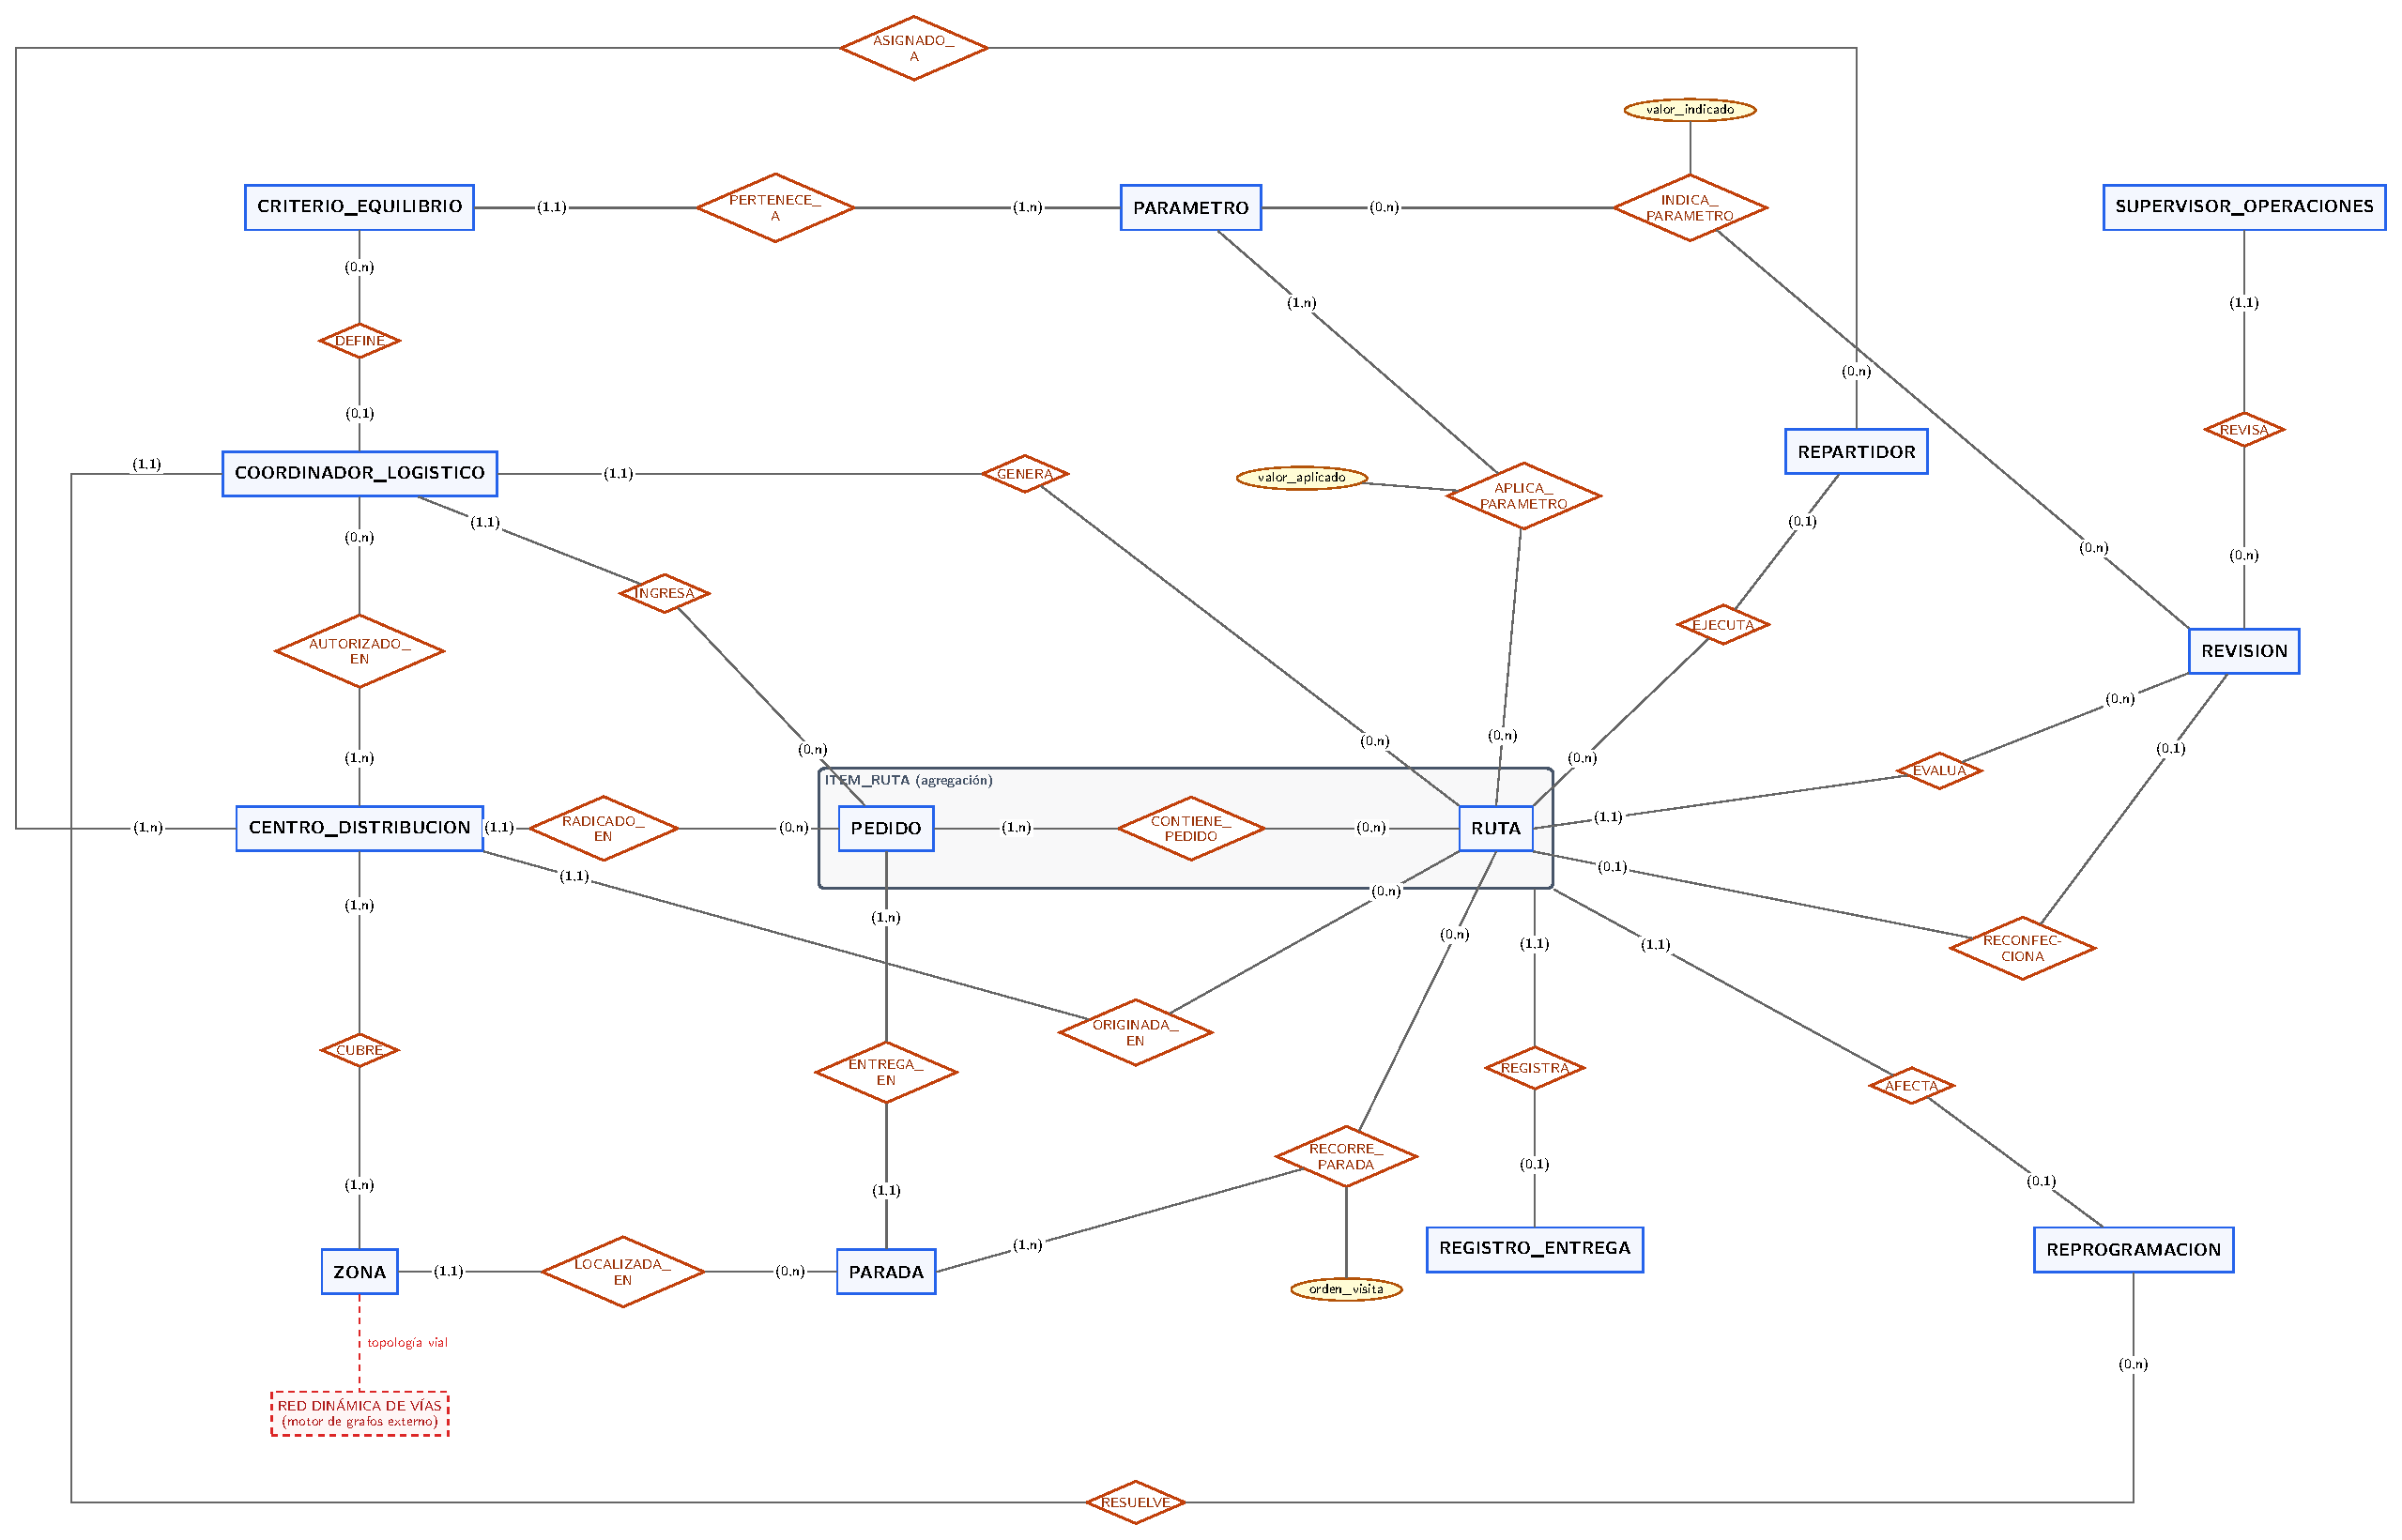
\includegraphics[width=\linewidth,height=0.94\textheight,keepaspectratio]{merx.pdf}
\caption{Modelo Entidad-Relación Extendido (MERX) del sistema.}
\label{fig:merx}
\end{figure}
\end{landscape}

\subsubsection*{Catálogo de entidades}
La clave primaria se subraya; \textit{(N)} indica que el atributo admite nulo.

\begin{longtable}{P{0.25\textwidth}P{0.40\textwidth}P{0.27\textwidth}}
\toprule
\textbf{Entidad} & \textbf{Descripción} & \textbf{Atributos}\\ \midrule
\endhead
\tabla{COORDINADOR\_LOGISTICO} & Actor que ingresa pedidos, define criterios de equilibrio, genera rutas y resuelve reprogramaciones. & \pk{id\_coordinador}, \campo{nombre\_coordinador}, \campo{especialidad}\\
\tabla{REPARTIDOR} & Operador de campo que ejecuta las rutas asignadas y registra el resultado de cada entrega. & \pk{id\_repartidor}, \campo{nombre\_repartidor}, \campo{edad}, \campo{flota}\\
\tabla{SUPERVISOR\_OPERACIONES} & Actor que revisa las rutas generadas, las aprueba o rechaza y puede indicar la confección de otra. & \pk{id\_supervisor}, \campo{nombre\_supervisor}, \campo{area\_control}\\
\tabla{CENTRO\_DISTRIBUCION} & Almacén donde radican los pedidos y desde el que parten las rutas. & \pk{id\_centro}, \campo{nombre\_centro}, \campo{programa\_logistico}\\
\tabla{ZONA} & Sector territorial atendido por uno o más centros. Sus conexiones viales se gestionan fuera del modelo relacional. & \pk{id\_zona}, \campo{nombre\_zona}\\
\tabla{PARADA} & Punto físico donde el vehículo se detiene para entregar uno o varios pedidos. & \pk{id\_parada}, \campo{direccion}\\
\tabla{PEDIDO} & Unidad de transporte ingresada por un coordinador y clasificada por tipo de entrega y prioridad. & \pk{id\_pedido}, \campo{descripcion}, \campo{tipo\_entrega}, \campo{prioridad}, \campo{peso\_kg}, \campo{fecha\_ingreso}, \campo{fecha\_hora\_limite}, \campo{estado\_pedido}\\
\tabla{CRITERIO\_EQUILIBRIO} & Regla de balanceo usada por el generador de rutas. Es preestablecida si no tiene coordinador autor (dato derivado). & \pk{id\_criterio}, \campo{nombre\_criterio}, \campo{descripcion\_criterio}\\
\tabla{PARAMETRO} & Condición atómica que forma parte de un criterio: una métrica calculable sobre la ruta, un operador de comparación y, si la métrica lo requiere, un tipo de entrega objetivo. & \pk{id\_parametro}, \campo{nombre\_parametro}, \campo{metrica}, \campo{operador}, \campo{tipo\_entrega\_objetivo} (N)\\
\tabla{RUTA} & Itinerario de reparto planificado para una jornada. Su estado se deriva de su última revisión. & \pk{id\_ruta}, \campo{fecha\_creacion}, \campo{fecha\_programada}, \campo{capacidad\_vehiculo\_kg}\\
\tabla{REVISION} & Acto de revisión de una ruta por un supervisor, con su decisión y observaciones. Una ruta puede tener varias. & \pk{id\_revision}, \campo{fecha\_hora\_revision}, \campo{decision}, \campo{observaciones\_revision}\\
\tabla{REGISTRO\_ENTREGA} & Constancia del intento de entrega de un pedido dentro de una ruta concreta. & \pk{id\_entrega}, \campo{fecha\_hora\_entrega}, \campo{resultado}, \campo{observaciones\_entrega}\\
\tabla{REPROGRAMACION} & Solicitud virtual de reprogramación de la entrega de un pedido dentro de una ruta, y su resolución manual por un coordinador. & \pk{id\_reprogramacion}, \campo{fecha\_solicitud}, \campo{motivo}, \campo{estado\_solicitud}, \campo{resultado\_manual} (N), \campo{fecha\_resolucion} (N)\\
\bottomrule
\end{longtable}

La unidad de cada parámetro queda determinada por su métrica (catálogo fijo de la aplicación), por lo que no se almacena: hacerlo introduciría la dependencia transitiva \campo{metrica} $\rightarrow$ \campo{unidad}.

\subsubsection*{Agregación ITEM\_RUTA}
La interrelación \tabla{CONTIENE\_PEDIDO} (RUTA--PEDIDO) se trata como una \textbf{agregación}, \tabla{ITEM\_RUTA} = [RUTA -- CONTIENE\_PEDIDO -- PEDIDO], que representa ``un pedido dentro de una ruta concreta''. Los registros de entrega y las reprogramaciones se asocian a esta agregación y no al pedido aislado. Así, un mismo pedido puede tener un intento y una reprogramación en cada ruta en la que figure, sin perder la historia de las anteriores.

\subsubsection*{Catálogo de interrelaciones}
{\small\setlength{\tabcolsep}{4pt}
\begin{longtable}{P{0.19\textwidth}P{0.23\textwidth}P{0.16\textwidth}P{0.12\textwidth}P{0.20\textwidth}}
\toprule
\textbf{Interrelación} & \textbf{Entidades} & \textbf{Cardinalidad} & \textbf{Atributos} & \textbf{Descripción}\\ \midrule
\endhead
AUTORIZADO\_EN & COORDINADOR -- CENTRO & Coord. (0,n) : (1,n) Centro & -- & Centros para los que el coordinador está autorizado a generar o validar rutas e ingresar pedidos.\\
ASIGNADO\_A & REPARTIDOR -- CENTRO & Rep. (0,n) : (1,n) Centro & -- & Centros en los que el repartidor puede recibir rutas.\\
CUBRE & CENTRO -- ZONA & Centro (1,n) : (1,n) Zona & -- & Cobertura territorial de cada centro.\\
INGRESA & COORDINADOR -- PEDIDO & Coord. (1,1) : (0,n) Pedido & -- & Coordinador que dio de alta el pedido.\\
RADICADO\_EN & CENTRO -- PEDIDO & Centro (1,1) : (0,n) Pedido & -- & Centro en el que se custodia el pedido.\\
ENTREGA\_EN & PEDIDO -- PARADA & Pedido (1,n) : (1,1) Parada & -- & Parada de destino del pedido.\\
LOCALIZADA\_EN & PARADA -- ZONA & Parada (0,n) : (1,1) Zona & -- & Zona de la parada; la zona de un pedido se obtiene por su parada.\\
DEFINE & COORDINADOR -- CRITERIO & Coord. (0,1) : (0,n) Criterio & -- & Autor del criterio; sin autor, el criterio es preestablecido.\\
PERTENECE\_A & PARAMETRO -- CRITERIO & Criterio (1,1) : (1,n) Parámetro & -- & Parámetros que componen cada criterio.\\
GENERA & COORDINADOR -- RUTA & Coord. (1,1) : (0,n) Ruta & -- & Coordinador que ejecutó la generación de la ruta.\\
ORIGINADA\_EN & CENTRO -- RUTA & Centro (1,1) : (0,n) Ruta & -- & Centro desde el que parte la ruta.\\
EJECUTA & REPARTIDOR -- RUTA & Rep. (0,1) : (0,n) Ruta & -- & Repartidor asignado a la ruta, una vez aprobada.\\
CONTIENE\_PEDIDO & RUTA -- PEDIDO & Ruta (0,n) : (1,n) Pedido & -- & Pedidos que transporta la ruta; un pedido puede figurar en varias rutas. Da lugar a ITEM\_RUTA.\\
RECORRE\_PARADA & RUTA -- PARADA & Ruta (0,n) : (1,n) Parada & \campo{orden\_visita} & Itinerario ordenado de paradas de la ruta.\\
APLICA\_PARAMETRO & RUTA -- PARAMETRO & Ruta (0,n) : (1,n) Parámetro & \campo{valor\_aplicado} & Valores de los parámetros usados al generar la ruta (configuración congelada).\\
REVISA & SUPERVISOR -- REVISION & Sup. (1,1) : (0,n) Revisión & -- & Supervisor que realiza la revisión.\\
EVALUA & RUTA -- REVISION & Ruta (1,1) : (0,n) Revisión & -- & Ruta sobre la que recae la revisión; conserva el historial.\\
INDICA\_PARAMETRO & REVISION -- PARAMETRO & Revisión (0,n) : (0,n) Parámetro & \campo{valor\_indicado} & Criterios que el supervisor indica al rechazar la ruta; su presencia constituye la solicitud de re-confección.\\
RECONFECCIONA & REVISION -- RUTA & Revisión (0,1) : (0,1) Ruta & -- & Ruta nueva confeccionada a partir de una revisión rechazada con solicitud de re-confección.\\
REGISTRA & ITEM\_RUTA -- REGISTRO\_ENTREGA & Ítem (1,1) : (0,1) Registro & -- & Resultado del intento de entrega de un pedido en una ruta.\\
AFECTA & ITEM\_RUTA -- REPROGRAMACION & Ítem (1,1) : (0,1) Reprog. & -- & Pedido-en-ruta cuya entrega se solicita reprogramar.\\
RESUELVE & COORDINADOR -- REPROGRAMACION & Coord. (1,1) : (0,n) Reprog. & -- & Coordinador indicado por el repartidor para resolver la solicitud.\\
\bottomrule
\end{longtable}
}

\subsubsection*{Elementos derivados que no forman parte del modelo}
\begin{longtable}{P{0.28\textwidth}P{0.32\textwidth}P{0.32\textwidth}}
\toprule
\textbf{Elemento} & \textbf{Se obtiene a partir de} & \textbf{Motivo de su exclusión}\\ \midrule
\endhead
Zona del pedido & ENTREGA\_EN + LOCALIZADA\_EN & Una interrelación directa pedido--zona sería redundante.\\
Repartidor que solicita la reprogramación & AFECTA $\rightarrow$ ruta $\rightarrow$ EJECUTA & Quien solicita es el repartidor que ejecuta la ruta del pedido; almacenarlo exigiría controlar que coincidan.\\
Criterios aplicados a una ruta & APLICA\_PARAMETRO + PERTENECE\_A & Cada parámetro pertenece a un único criterio.\\
Estado de la ruta & Última REVISION de la ruta y existencia de INDICA\_PARAMETRO en ella (sección~\ref{sec:semanticas}) & Se evita la inconsistencia entre el estado y las revisiones.\\
Fecha de validación de la ruta & \campo{fecha\_hora\_revision} de la revisión aprobatoria & Reemplazada por el historial de revisiones.\\
Criterio preestablecido & Ausencia de DEFINE & Redundante con la autoría.\\
Registro fallido que motiva una reprogramación & REGISTRA sobre el mismo ITEM\_RUTA & Ambos cuelgan del mismo pedido-en-ruta.\\
Disponibilidad del repartidor & Almacén clave-valor (sección~\ref{sec:nosql}) & Estado operativo transitorio; no se duplica en el modelo relacional.\\
\bottomrule
\end{longtable}

\subsubsection*{Justificación de la cardinalidad de REPROGRAMACION}
El enunciado pide que el repartidor pueda ``solicitar de forma virtual una reprogramación de entrega'', sin condicionarla a un intento fallido previo. Por eso la reprogramación no exige un registro de entrega fallido: se asocia al pedido-en-ruta (AFECTA, (1,1)). Esto cubre tanto la solicitud posterior a un intento fallido como la solicitud anticipada, por ejemplo cuando el repartidor sabe antes de llegar que el destinatario no estará. Si el pedido-en-ruta ya tiene un registro de entrega, este debe ser \textit{Fallido} (sección~\ref{sec:semanticas}).

% =====================================================================
\section{Especificación de las restricciones de integridad}

Las restricciones se derivan de los requisitos, de las cardinalidades del MERX y de las dependencias funcionales de la sección~\ref{sec:valoracion}. Las que no pueden expresarse con claves y restricciones de dominio se implementan mediante disparadores o en la capa de servicios, y así se indica.

\subsection{Restricciones de unicidad}
\begin{itemize}
\item Toda tabla tiene una clave primaria única y no nula.
\item \textbf{Claves alternativas:}
  \begin{itemize}
  \item En \tabla{RUTA\_PARADA}, el par (\campo{id\_ruta}, \campo{orden\_visita}) es único: dentro de una ruta no se repite la posición de visita.
  \item En \tabla{REGISTRO\_ENTREGA}, el par (\campo{id\_ruta}, \campo{id\_pedido}) es único: a lo sumo un registro por pedido-en-ruta.
  \item En \tabla{REPROGRAMACION}, el par (\campo{id\_ruta}, \campo{id\_pedido}) es único: a lo sumo una solicitud por pedido-en-ruta.
  \item En \tabla{RUTA}, \campo{id\_revision\_origen} es único cuando no es nulo: una revisión origina como máximo una ruta nueva.
  \end{itemize}
\item \textbf{Antiduplicados de pedidos (RF-17):} la combinación (\campo{id\_centro\_pedido}, \campo{id\_parada}, \campo{tipo\_entrega}, \campo{descripcion}, \campo{fecha\_ingreso}) es única, donde \campo{fecha\_ingreso} es una fecha (día, sin hora). Regla de negocio adoptada: dos pedidos son duplicados si radican en el mismo centro, van a la misma parada, son del mismo tipo de entrega, tienen la misma descripción y se ingresaron el mismo día. Si un remitente envía legítimamente varios bultos idénticos al mismo destino el mismo día, se registran como un único pedido cuya descripción indica la cantidad.
\item \textbf{Una ruta, un repartidor (RF-17):} queda garantizado estructuralmente, porque \campo{id\_repartidor} es un atributo monovaluado de \tabla{RUTA}.
\end{itemize}

\subsection{Restricciones semánticas}\label{sec:semanticas}

\textbf{Dominios}
\begin{itemize}
\item \campo{tipo\_entrega}, \campo{tipo\_entrega\_objetivo} $\in$ \{Paquetería, Documentos, Perecederos\}.
\item \campo{prioridad} $\in$ \{Baja, Media, Urgente\}; \campo{decision} $\in$ \{Aprobada, Rechazada\}; \campo{resultado} $\in$ \{Exitoso, Fallido\}.
\item \campo{estado\_pedido} $\in$ \{Pendiente, En ruta, Entregado, Devuelto\}; \campo{estado\_solicitud} $\in$ \{Pendiente, En proceso, Resuelta\}; \campo{resultado\_manual} $\in$ \{Reasignado, Reprogramado, Devuelto al almacén\}.
\item \campo{metrica} $\in$ \{CANTIDAD\_PEDIDOS, PROPORCION\_TIPO, CANTIDAD\_ZONAS, PESO\_TOTAL, CANTIDAD\_PARADAS\}; \campo{operador} $\in$ \{$\le$, $\ge$, $=$\}.
\item \campo{peso\_kg} $> 0$, \campo{capacidad\_vehiculo\_kg} $> 0$, \campo{orden\_visita} $\ge 1$, \campo{edad} $\ge 18$.
\end{itemize}

\textbf{Parámetros y criterios}
\begin{itemize}
\item \campo{tipo\_entrega\_objetivo} no es nulo si y solo si \campo{metrica} = PROPORCION\_TIPO.
\item Si \campo{metrica} = PROPORCION\_TIPO, entonces \campo{valor\_aplicado} y \campo{valor\_indicado} $\in [0,1]$.
\end{itemize}

\textbf{Revisión y re-confección de rutas}
\begin{itemize}
\item \textbf{Estado de la ruta (derivado, RF-12).} El enunciado agrupa ``Rechazada / En Modificación'' en un solo valor; aquí se distinguen dos situaciones con consecuencias diferentes. Una revisión rechazada \emph{solicita re-confección} si tiene al menos un parámetro indicado en \tabla{INDICA\_PARAMETRO}. El estado de una ruta es:
  \begin{itemize}
  \item \textit{Pendiente de Aprobación}: la ruta no tiene revisiones;
  \item \textit{Aprobada}: su última revisión tiene decisión \textit{Aprobada};
  \item \textit{Rechazada}: su última revisión tiene decisión \textit{Rechazada} sin solicitud de re-confección; la ruta queda descartada y sus pedidos pueden incluirse en otras rutas;
  \item \textit{En Modificación}: su última revisión tiene decisión \textit{Rechazada} con solicitud de re-confección; se confecciona otra ruta con los criterios indicados, que queda vinculada mediante \tabla{RECONFECCIONA}.
  \end{itemize}
\item Una ruta puede recibir nuevas revisiones (por ejemplo, para revocar una aprobación antes de iniciar el reparto) mientras no tenga registros de entrega ni exista una ruta reconfeccionada a partir de ella. La última revisión, por \campo{fecha\_hora\_revision}, determina el estado.
\item \campo{observaciones\_revision} no es nulo cuando \campo{decision} = Rechazada.
\item \tabla{INDICA\_PARAMETRO} solo se registra en revisiones con decisión \textit{Rechazada}.
\item \campo{id\_revision\_origen} de una ruta solo puede referenciar una revisión con decisión \textit{Rechazada} que solicita re-confección. La ruta nueva pertenece al mismo centro que la ruta revisada y aplica, para cada parámetro indicado en esa revisión, el valor indicado por el supervisor (\campo{valor\_aplicado} = \campo{valor\_indicado}). \trig
\end{itemize}

\textbf{Composición de la ruta}
\begin{itemize}
\item \textbf{Capacidad (RF-07):} la suma de \campo{peso\_kg} de los pedidos contenidos en una ruta no supera su \campo{capacidad\_vehiculo\_kg}. \trig
\item \textbf{Coherencia ruta--parada:} el conjunto de paradas de una ruta en \tabla{RUTA\_PARADA} coincide exactamente con el conjunto de paradas de destino de sus pedidos en \tabla{RUTA\_PEDIDO}: no hay paradas sin pedidos ni pedidos sin su parada en el itinerario. \trig
\item \textbf{Orden de visita:} en cada ruta, los valores de \campo{orden\_visita} forman la secuencia $1, 2, \dots, k$, donde $k$ es la cantidad de paradas.
\item \textbf{Mismo centro:} los pedidos de una ruta radican en el centro de la ruta (\campo{id\_centro\_pedido} = \campo{id\_centro\_ruta}), y la zona de cada parada de la ruta está cubierta por ese centro (\tabla{CUBRE}).
\item \textbf{Pedido vigente único:} un pedido no puede figurar a la vez en dos rutas que estén \textit{Pendientes de Aprobación} o \textit{Aprobadas} y en las que todavía no tenga registro de entrega. \trig
\end{itemize}

\textbf{Autorizaciones de los actores}
\begin{itemize}
\item El coordinador que ingresa un pedido está autorizado en el centro del pedido, y el que genera una ruta está autorizado en el centro de la ruta (\tabla{AUTORIZADO\_EN}).
\item El coordinador que resuelve una reprogramación está autorizado en el centro de la ruta del pedido afectado.
\item Solo el coordinador que ingresó un pedido (\campo{id\_coord\_ingreso}) puede modificar su clasificación (\campo{prioridad}, \campo{tipo\_entrega} y parada de destino, de la que se deriva la zona). Se controla en la capa de servicios.
\item Solo las rutas \textit{Aprobadas} tienen repartidor, y este está asignado al centro de la ruta (\tabla{ASIGNADO\_A}).
\item Un repartidor no puede tener dos rutas \textit{Aprobadas} con la misma \campo{fecha\_programada} (RF-17). \trig
\end{itemize}

\textbf{Entregas y reprogramaciones}
\begin{itemize}
\item Solo se registran entregas y reprogramaciones sobre pedidos-en-ruta de rutas \textit{Aprobadas} con repartidor asignado.
\item Si un pedido-en-ruta tiene a la vez registro de entrega y reprogramación, el registro tiene resultado \textit{Fallido}.
\item \campo{resultado\_manual} y \campo{fecha\_resolucion} no son nulos si y solo si \campo{estado\_solicitud} = Resuelta.
\end{itemize}

\textbf{Concepto derivado}
\begin{itemize}
\item Un pedido-en-ruta se entregó a tiempo si y solo si su registro tiene \campo{resultado} = Exitoso y \campo{fecha\_hora\_entrega} $\le$ \campo{fecha\_hora\_limite} del pedido. Esta condición no se almacena; se calcula en las consultas RI-04 y RI-06.
\end{itemize}

\subsection{Restricciones temporales}
\begin{itemize}
\item La \campo{fecha\_programada} de una ruta no es anterior a su \campo{fecha\_creacion}.
\item La fecha de \campo{fecha\_hora\_limite} de un pedido no es anterior a su \campo{fecha\_ingreso}.
\item La \campo{fecha\_ingreso} de un pedido no es posterior a la \campo{fecha\_creacion} de ninguna ruta que lo contenga.
\item La \campo{fecha\_hora\_revision} de una revisión es posterior a la \campo{fecha\_creacion} de la ruta evaluada. Las revisiones de una misma ruta tienen fechas distintas, lo que permite determinar cuál es la última.
\item La \campo{fecha\_creacion} de una ruta reconfeccionada es posterior a la \campo{fecha\_hora\_revision} de su revisión de origen.
\item La \campo{fecha\_hora\_entrega} de un registro no es anterior a la \campo{fecha\_programada} de su ruta ni a la \campo{fecha\_hora\_revision} de la revisión que la aprobó.
\item La \campo{fecha\_solicitud} de una reprogramación es posterior a la revisión aprobatoria de la ruta y, si existe registro de entrega del mismo pedido-en-ruta, no es anterior a su \campo{fecha\_hora\_entrega}.
\item La \campo{fecha\_resolucion} de una reprogramación es posterior a su \campo{fecha\_solicitud}.
\end{itemize}

\subsection{Restricciones de integridad referencial}
\begin{itemize}
\item Todas las claves foráneas del esquema de la sección~\ref{sec:esquema} referencian una clave primaria existente.
\item Admiten nulo: \campo{id\_repartidor} de \tabla{RUTA} (se completa al asignar la ruta aprobada), \campo{id\_revision\_origen} de \tabla{RUTA} (solo existe en rutas reconfeccionadas) e \campo{id\_coord\_autor} de \tabla{CRITERIO\_EQUILIBRIO} (nulo en los criterios preestablecidos).
\item \tabla{REGISTRO\_ENTREGA} y \tabla{REPROGRAMACION} referencian a \tabla{RUTA\_PEDIDO} mediante la clave foránea compuesta (\campo{id\_ruta}, \campo{id\_pedido}), lo que garantiza que solo se registren intentos y solicitudes sobre pedidos que efectivamente pertenecen a la ruta.
\item Las claves foráneas que designan coordinadores con distintos roles (\campo{id\_coord\_ingreso}, \campo{id\_coord\_generador}, \campo{id\_coord\_autor}, \campo{id\_coord\_resolutor}) referencian \campo{id\_coordinador}; las que designan centros (\campo{id\_centro\_pedido}, \campo{id\_centro\_ruta}) referencian \campo{id\_centro}.
\item \textbf{Borrado restringido:} no se elimina un centro con pedidos, rutas o actores asociados; un pedido que figure en alguna ruta; una ruta con revisiones; un coordinador, repartidor o supervisor referenciado por pedidos, rutas, criterios, revisiones o reprogramaciones; ni un parámetro aplicado o indicado en alguna ruta o revisión.
\item \textbf{Borrado en cascada:} al eliminar una ruta sin revisiones (descartada antes de ser revisada) se eliminan sus filas en \tabla{RUTA\_PEDIDO}, \tabla{RUTA\_PARADA} y \tabla{RUTA\_PARAMETRO}.
\end{itemize}

% =====================================================================
\section{Valoración de la corrección del diseño}\label{sec:valoracion}

\subsection{Universo de atributos y dependencias funcionales}

Para respetar la hipótesis de la relación universal (cada nombre de atributo tiene un único significado), los atributos que referencian una misma entidad con roles distintos reciben nombres distintos: \campo{id\_coord\_ingreso} (INGRESA), \campo{id\_coord\_generador} (GENERA), \campo{id\_coord\_autor} (DEFINE) e \campo{id\_coord\_resolutor} (RESUELVE); \campo{id\_centro\_pedido} (RADICADO\_EN) e \campo{id\_centro\_ruta} (ORIGINADA\_EN); e \campo{id\_revision\_origen} (RECONFECCIONA). Si se usara el mismo nombre \campo{id\_coordinador} en todos los casos, de \campo{id\_reprogramacion} $\rightarrow$ \campo{id\_ruta} e \campo{id\_ruta} $\rightarrow$ \campo{id\_coordinador} se inferiría erróneamente que quien resuelve una reprogramación es quien generó la ruta.

\textbf{Universo de atributos $U$:}

{\raggedright\small
$U$ = \{ \campo{id\_coordinador}, \campo{nombre\_coordinador}, \campo{especialidad}, \campo{id\_repartidor}, \campo{nombre\_repartidor}, \campo{edad}, \campo{flota}, \campo{id\_supervisor}, \campo{nombre\_supervisor}, \campo{area\_control}, \campo{id\_centro}, \campo{nombre\_centro}, \campo{programa\_logistico}, \campo{id\_zona}, \campo{nombre\_zona}, \campo{id\_parada}, \campo{direccion}, \campo{id\_pedido}, \campo{descripcion}, \campo{tipo\_entrega}, \campo{prioridad}, \campo{peso\_kg}, \campo{fecha\_ingreso}, \campo{fecha\_hora\_limite}, \campo{estado\_pedido}, \campo{id\_coord\_ingreso}, \campo{id\_centro\_pedido}, \campo{id\_criterio}, \campo{nombre\_criterio}, \campo{descripcion\_criterio}, \campo{id\_coord\_autor}, \campo{id\_parametro}, \campo{nombre\_parametro}, \campo{metrica}, \campo{operador}, \campo{tipo\_entrega\_objetivo}, \campo{id\_ruta}, \campo{fecha\_creacion}, \campo{fecha\_programada}, \campo{capacidad\_vehiculo\_kg}, \campo{id\_coord\_generador}, \campo{id\_centro\_ruta}, \campo{id\_revision\_origen}, \campo{id\_revision}, \campo{fecha\_hora\_revision}, \campo{decision}, \campo{observaciones\_revision}, \campo{id\_entrega}, \campo{fecha\_hora\_entrega}, \campo{resultado}, \campo{observaciones\_entrega}, \campo{id\_reprogramacion}, \campo{fecha\_solicitud}, \campo{motivo}, \campo{estado\_solicitud}, \campo{resultado\_manual}, \campo{fecha\_resolucion}, \campo{id\_coord\_resolutor}, \campo{orden\_visita}, \campo{valor\_aplicado}, \campo{valor\_indicado} \}
\par}

Las dependencias funcionales se extraen del MERX aplicando tres reglas.

\textbf{Regla 1: dependencias de entidades (clave $\rightarrow$ atributos propios)}
{\raggedright
\begin{itemize}[leftmargin=1.2cm,labelwidth=1cm,align=left]
\df{1}{\campo{id\_coordinador}}{\campo{nombre\_coordinador}, \campo{especialidad}}
\df{2}{\campo{id\_repartidor}}{\campo{nombre\_repartidor}, \campo{edad}, \campo{flota}}
\df{3}{\campo{id\_supervisor}}{\campo{nombre\_supervisor}, \campo{area\_control}}
\df{4}{\campo{id\_centro}}{\campo{nombre\_centro}, \campo{programa\_logistico}}
\df{5}{\campo{id\_zona}}{\campo{nombre\_zona}}
\df{6}{\campo{id\_parada}}{\campo{direccion}}
\df{7}{\campo{id\_pedido}}{\campo{descripcion}, \campo{tipo\_entrega}, \campo{prioridad}, \campo{peso\_kg}, \campo{fecha\_ingreso}, \campo{fecha\_hora\_limite}, \campo{estado\_pedido}}
\df{8}{\campo{id\_criterio}}{\campo{nombre\_criterio}, \campo{descripcion\_criterio}}
\df{9}{\campo{id\_parametro}}{\campo{nombre\_parametro}, \campo{metrica}, \campo{operador}, \campo{tipo\_entrega\_objetivo}}
\df{10}{\campo{id\_ruta}}{\campo{fecha\_creacion}, \campo{fecha\_programada}, \campo{capacidad\_vehiculo\_kg}}
\df{11}{\campo{id\_revision}}{\campo{fecha\_hora\_revision}, \campo{decision}, \campo{observaciones\_revision}}
\df{12}{\campo{id\_entrega}}{\campo{fecha\_hora\_entrega}, \campo{resultado}, \campo{observaciones\_entrega}}
\df{13}{\campo{id\_reprogramacion}}{\campo{fecha\_solicitud}, \campo{motivo}, \campo{estado\_solicitud}, \campo{resultado\_manual}, \campo{fecha\_resolucion}}
\end{itemize}
\par}

\textbf{Regla 2: interrelaciones con un extremo de cardinalidad máxima 1}
{\raggedright
\begin{itemize}[leftmargin=1.2cm,labelwidth=1cm,align=left]
\df{14}{\campo{id\_pedido}}{\campo{id\_coord\_ingreso}} \hfill (INGRESA)
\df{15}{\campo{id\_pedido}}{\campo{id\_centro\_pedido}} \hfill (RADICADO\_EN)
\df{16}{\campo{id\_pedido}}{\campo{id\_parada}} \hfill (ENTREGA\_EN)
\df{17}{\campo{id\_parada}}{\campo{id\_zona}} \hfill (LOCALIZADA\_EN)
\df{18}{\campo{id\_criterio}}{\campo{id\_coord\_autor}} \hfill (DEFINE)
\df{19}{\campo{id\_parametro}}{\campo{id\_criterio}} \hfill (PERTENECE\_A)
\df{20}{\campo{id\_ruta}}{\campo{id\_coord\_generador}} \hfill (GENERA)
\df{21}{\campo{id\_ruta}}{\campo{id\_centro\_ruta}} \hfill (ORIGINADA\_EN)
\df{22}{\campo{id\_ruta}}{\campo{id\_repartidor}} \hfill (EJECUTA)
\df{23}{\campo{id\_revision}}{\campo{id\_supervisor}} \hfill (REVISA)
\df{24}{\campo{id\_revision}}{\campo{id\_ruta}} \hfill (EVALUA)
\df{25}{\campo{id\_ruta}}{\campo{id\_revision\_origen}} \hfill (RECONFECCIONA)
\df{26}{\campo{id\_entrega}}{\campo{id\_ruta}, \campo{id\_pedido}} \hfill (REGISTRA)
\df{27}{\campo{id\_reprogramacion}}{\campo{id\_ruta}, \campo{id\_pedido}} \hfill (AFECTA)
\df{28}{\campo{id\_reprogramacion}}{\campo{id\_coord\_resolutor}} \hfill (RESUELVE)
\end{itemize}
\par}

En las interrelaciones 1:1 con un extremo opcional (RECONFECCIONA, REGISTRA, AFECTA) se extrae la dependencia desde la entidad de participación obligatoria. La dependencia inversa (por ejemplo, \{\campo{id\_ruta}, \campo{id\_pedido}\} $\rightarrow$ \campo{id\_entrega}) solo se cumple sobre las tuplas existentes y se expresa como clave alternativa (sección 3.1). Incluirla en $F$ haría que el algoritmo de síntesis fusionara en un único esquema entidades con existencia independiente: registros de entrega, reprogramaciones y la pertenencia pedido--ruta.

\textbf{Regla 3: atributos propios de interrelaciones N:M}
{\raggedright
\begin{itemize}[leftmargin=1.2cm,labelwidth=1cm,align=left]
\df{29}{\campo{id\_ruta}, \campo{id\_parada}}{\campo{orden\_visita}}
\df{30}{\campo{id\_ruta}, \campo{orden\_visita}}{\campo{id\_parada}}
\df{31}{\campo{id\_ruta}, \campo{id\_parametro}}{\campo{valor\_aplicado}}
\df{32}{\campo{id\_revision}, \campo{id\_parametro}}{\campo{valor\_indicado}}
\end{itemize}
\par}

$f_{30}$ expresa que en una ruta cada posición de visita corresponde a una sola parada.

\textbf{Regla 4: interrelaciones N:M sin atributos.} En AUTORIZADO\_EN, ASIGNADO\_A, CUBRE y CONTIENE\_PEDIDO ningún extremo determina al otro: un coordinador está autorizado en varios centros y un centro tiene varios coordinadores. Siguiendo el procedimiento del curso, cada una se representa en $F$ mediante la dependencia trivial de su llave sobre sí misma. Esta dependencia expresa que el par de identificadores es un hecho que debe almacenarse, y da origen al esquema de la interrelación en la síntesis:
{\raggedright
\begin{itemize}[leftmargin=1.2cm,labelwidth=1cm,align=left]
\df{33}{\campo{id\_coordinador}, \campo{id\_centro}}{\campo{id\_coordinador}, \campo{id\_centro}} \hfill (AUTORIZADO\_EN)
\df{34}{\campo{id\_repartidor}, \campo{id\_centro}}{\campo{id\_repartidor}, \campo{id\_centro}} \hfill (ASIGNADO\_A)
\df{35}{\campo{id\_centro}, \campo{id\_zona}}{\campo{id\_centro}, \campo{id\_zona}} \hfill (CUBRE)
\df{36}{\campo{id\_ruta}, \campo{id\_pedido}}{\campo{id\_ruta}, \campo{id\_pedido}} \hfill (CONTIENE\_PEDIDO)
\end{itemize}
\par}
Las interrelaciones N:M con atributos (RECORRE\_PARADA, APLICA\_PARAMETRO, INDICA\_PARAMETRO) no necesitan dependencia trivial, porque $f_{29}$--$f_{32}$ ya generan su esquema con la misma llave. Así, $F = \{f_1, \dots, f_{36}\}$.

% ---------------------------------------------------------------------
\subsection{Cubrimiento minimal}\label{sec:cubrimiento}

Se obtiene un cubrimiento minimal $F_m$ de $F = \{f_1,\dots,f_{36}\}$ en tres pasos: (1) dejar un solo atributo en cada consecuente; (2) eliminar los atributos superfluos de los determinantes; (3) eliminar las dependencias redundantes. Los pasos se aplican a las dependencias no triviales $f_1$--$f_{32}$. Las dependencias triviales $f_{33}$--$f_{36}$ se conservan tal cual, como en el ejemplo de la conferencia, donde \#E,\#A $\rightarrow$ \#E,\#A permanece en el cubrimiento minimal. No aportan información sobre $F^+$ (se deducen por reflexividad), pero registran las interrelaciones N:M que la síntesis debe convertir en esquemas. Para abreviar se usan las siguientes clausuras, calculadas sobre $F$:

{\raggedright\small
\begin{itemize}
\item $C_{\text{parada}} = \{\campo{id\_parada}\}^+ = \{\campo{id\_parada}, \campo{direccion}, \campo{id\_zona}, \campo{nombre\_zona}\}$ (por $f_6$, $f_{17}$, $f_5$).
\item $C_{\text{pedido}} = \{\campo{id\_pedido}\}^+ = \{\campo{id\_pedido}$, atributos de $f_7$, \campo{id\_coord\_ingreso}, \campo{id\_centro\_pedido}$\} \cup C_{\text{parada}}$ (por $f_7$, $f_{14}$--$f_{16}$).
\item $C_{\text{ruta}} = \{\campo{id\_ruta}\}^+ = \{\campo{id\_ruta}$, \campo{fecha\_creacion}, \campo{fecha\_programada}, \campo{capacidad\_vehiculo\_kg}, \campo{id\_coord\_generador}, \campo{id\_centro\_ruta}, \campo{id\_repartidor}, \campo{nombre\_repartidor}, \campo{edad}, \campo{flota}, \campo{id\_revision\_origen}$\}$ (por $f_{10}$, $f_{20}$--$f_{22}$, $f_2$, $f_{25}$).
\item $C_{\text{param}} = \{\campo{id\_parametro}\}^+ = \{\campo{id\_parametro}$, atributos de $f_9$, \campo{id\_criterio}, \campo{nombre\_criterio}, \campo{descripcion\_criterio}, \campo{id\_coord\_autor}$\}$ (por $f_9$, $f_{19}$, $f_8$, $f_{18}$).
\item $C_{\text{revision}} = \{\campo{id\_revision}\}^+ = \{\campo{id\_revision}$, atributos de $f_{11}$, \campo{id\_supervisor}, \campo{nombre\_supervisor}, \campo{area\_control}$\} \cup C_{\text{ruta}}$ (por $f_{11}$, $f_{23}$, $f_3$, $f_{24}$).
\end{itemize}
\par}

\subsubsection*{Paso 1: consecuentes unitarios ($F_1$)}
Por la regla de descomposición ($X \rightarrow YZ$ implica $X \rightarrow Y$ y $X \rightarrow Z$), cada dependencia con varios atributos en el consecuente se sustituye por una dependencia por atributo. Las dependencias $f_{14}$--$f_{25}$ y $f_{28}$--$f_{32}$ ya tienen consecuente unitario y se conservan. $F_1$ tiene 59 dependencias elementales.

{\small\raggedright
\begin{longtable}{P{0.10\textwidth}P{0.82\textwidth}}
\toprule
\textbf{En $F$} & \textbf{Dependencias elementales de $F_1$}\\ \midrule
\endhead
$f_1$ & $f_{1.1}$: \campo{id\_coordinador} $\rightarrow$ \campo{nombre\_coordinador};\; $f_{1.2}$: \campo{id\_coordinador} $\rightarrow$ \campo{especialidad}\\
$f_2$ & $f_{2.1}$--$f_{2.3}$: \campo{id\_repartidor} $\rightarrow$ \campo{nombre\_repartidor} $\mid$ \campo{edad} $\mid$ \campo{flota}\\
$f_3$ & $f_{3.1}$, $f_{3.2}$: \campo{id\_supervisor} $\rightarrow$ \campo{nombre\_supervisor} $\mid$ \campo{area\_control}\\
$f_4$ & $f_{4.1}$, $f_{4.2}$: \campo{id\_centro} $\rightarrow$ \campo{nombre\_centro} $\mid$ \campo{programa\_logistico}\\
$f_5$, $f_6$ & ya unitarias: \campo{id\_zona} $\rightarrow$ \campo{nombre\_zona};\; \campo{id\_parada} $\rightarrow$ \campo{direccion}\\
$f_7$ & $f_{7.1}$--$f_{7.7}$: \campo{id\_pedido} $\rightarrow$ \campo{descripcion} $\mid$ \campo{tipo\_entrega} $\mid$ \campo{prioridad} $\mid$ \campo{peso\_kg} $\mid$ \campo{fecha\_ingreso} $\mid$ \campo{fecha\_hora\_limite} $\mid$ \campo{estado\_pedido}\\
$f_8$ & $f_{8.1}$, $f_{8.2}$: \campo{id\_criterio} $\rightarrow$ \campo{nombre\_criterio} $\mid$ \campo{descripcion\_criterio}\\
$f_9$ & $f_{9.1}$--$f_{9.4}$: \campo{id\_parametro} $\rightarrow$ \campo{nombre\_parametro} $\mid$ \campo{metrica} $\mid$ \campo{operador} $\mid$ \campo{tipo\_entrega\_objetivo}\\
$f_{10}$ & $f_{10.1}$--$f_{10.3}$: \campo{id\_ruta} $\rightarrow$ \campo{fecha\_creacion} $\mid$ \campo{fecha\_programada} $\mid$ \campo{capacidad\_vehiculo\_kg}\\
$f_{11}$ & $f_{11.1}$--$f_{11.3}$: \campo{id\_revision} $\rightarrow$ \campo{fecha\_hora\_revision} $\mid$ \campo{decision} $\mid$ \campo{observaciones\_revision}\\
$f_{12}$ & $f_{12.1}$--$f_{12.3}$: \campo{id\_entrega} $\rightarrow$ \campo{fecha\_hora\_entrega} $\mid$ \campo{resultado} $\mid$ \campo{observaciones\_entrega}\\
$f_{13}$ & $f_{13.1}$--$f_{13.5}$: \campo{id\_reprogramacion} $\rightarrow$ \campo{fecha\_solicitud} $\mid$ \campo{motivo} $\mid$ \campo{estado\_solicitud} $\mid$ \campo{resultado\_manual} $\mid$ \campo{fecha\_resolucion}\\
$f_{26}$ & $f_{26.1}$: \campo{id\_entrega} $\rightarrow$ \campo{id\_ruta};\; $f_{26.2}$: \campo{id\_entrega} $\rightarrow$ \campo{id\_pedido}\\
$f_{27}$ & $f_{27.1}$: \campo{id\_reprogramacion} $\rightarrow$ \campo{id\_ruta};\; $f_{27.2}$: \campo{id\_reprogramacion} $\rightarrow$ \campo{id\_pedido}\\
\bottomrule
\end{longtable}
}

\subsubsection*{Paso 2: eliminación de atributos superfluos en los determinantes ($F_2$)}
Un atributo $B$ del determinante de $X \rightarrow A$ es superfluo si $A \in (X - \{B\})^+$. Solo $f_{29}$--$f_{32}$ tienen determinante compuesto, y para cada una se prueba quitar cada atributo:

{\small
\begin{longtable}{P{0.13\textwidth}P{0.17\textwidth}P{0.40\textwidth}P{0.20\textwidth}}
\toprule
\textbf{Dependencia} & \textbf{Se quita} & \textbf{Clausura del resto} & \textbf{¿Contiene el consecuente?}\\ \midrule
\endhead
$f_{29}$ & \campo{id\_parada} & $\{\campo{id\_ruta}\}^+ = C_{\text{ruta}}$ & No (\campo{orden\_visita})\\
$f_{29}$ & \campo{id\_ruta} & $\{\campo{id\_parada}\}^+ = C_{\text{parada}}$ & No\\
$f_{30}$ & \campo{orden\_visita} & $C_{\text{ruta}}$ & No (\campo{id\_parada})\\
$f_{30}$ & \campo{id\_ruta} & $\{\campo{orden\_visita}\}^+ = \{\campo{orden\_visita}\}$ & No\\
$f_{31}$ & \campo{id\_parametro} & $C_{\text{ruta}}$ & No (\campo{valor\_aplicado})\\
$f_{31}$ & \campo{id\_ruta} & $C_{\text{param}}$ & No\\
$f_{32}$ & \campo{id\_parametro} & $C_{\text{revision}}$ & No (\campo{valor\_indicado})\\
$f_{32}$ & \campo{id\_revision} & $C_{\text{param}}$ & No\\
\bottomrule
\end{longtable}
}

Ningún determinante tiene atributos superfluos, por lo que $F_2 = F_1$.

\subsubsection*{Paso 3: eliminación de dependencias redundantes ($F_3$)}
Una dependencia $g: X \rightarrow A$ de $F_2$ es redundante si $A \in X^+$, calculando la clausura en $F_2 - \{g\}$.

\textbf{Lema.} Si $A \notin X$ y $A$ es consecuente únicamente de $g$, entonces $g$ no es redundante. \textit{Demostración:} el cálculo de $X^+$ en $F_2 - \{g\}$ parte de $X$ y solo incorpora consecuentes de dependencias de $F_2 - \{g\}$; como ninguna tiene a $A$ por consecuente y $A \notin X$, resulta $A \notin X^+$. $\square$

En $F_2$, cada atributo es consecuente de una sola dependencia, excepto \campo{id\_ruta} ($f_{24}$, $f_{26.1}$, $f_{27.1}$), \campo{id\_pedido} ($f_{26.2}$, $f_{27.2}$) e \campo{id\_parada} ($f_{16}$, $f_{30}$). Por el lema, las otras 52 dependencias no son redundantes. Las 7 restantes se comprueban una a una:

{\small
\begin{longtable}{P{0.25\textwidth}P{0.50\textwidth}P{0.15\textwidth}}
\toprule
\textbf{$g$} & \textbf{$X^+$ en $F_2 - \{g\}$} & \textbf{¿Redundante?}\\ \midrule
\endhead
$f_{24}$: \campo{id\_revision} $\rightarrow$ \campo{id\_ruta} & $\{\campo{id\_revision}$, atributos de $f_{11}$, \campo{id\_supervisor}, \campo{nombre\_supervisor}, \campo{area\_control}$\}$ & No\\
$f_{26.1}$: \campo{id\_entrega} $\rightarrow$ \campo{id\_ruta} & $\{\campo{id\_entrega}$, atributos de $f_{12}\} \cup C_{\text{pedido}}$ & No\\
$f_{26.2}$: \campo{id\_entrega} $\rightarrow$ \campo{id\_pedido} & $\{\campo{id\_entrega}$, atributos de $f_{12}\} \cup C_{\text{ruta}}$ & No\\
$f_{27.1}$: \campo{id\_reprogramacion} $\rightarrow$ \campo{id\_ruta} & $\{\campo{id\_reprogramacion}$, atributos de $f_{13}$, \campo{id\_coord\_resolutor}$\} \cup C_{\text{pedido}}$ & No\\
$f_{27.2}$: \campo{id\_reprogramacion} $\rightarrow$ \campo{id\_pedido} & $\{\campo{id\_reprogramacion}$, atributos de $f_{13}$, \campo{id\_coord\_resolutor}$\} \cup C_{\text{ruta}}$ & No\\
$f_{16}$: \campo{id\_pedido} $\rightarrow$ \campo{id\_parada} & $\{\campo{id\_pedido}$, atributos de $f_7$, \campo{id\_coord\_ingreso}, \campo{id\_centro\_pedido}$\}$ & No\\
$f_{30}$: \campo{id\_ruta}, \campo{orden\_visita} $\rightarrow$ \campo{id\_parada} & $C_{\text{ruta}} \cup \{\campo{orden\_visita}\}$ ($f_{29}$ no se aplica porque exige \campo{id\_parada}) & No\\
\bottomrule
\end{longtable}
}

Ninguna dependencia no trivial es redundante: $F_3 = F_2 = F_1$, con 59 dependencias elementales. El cubrimiento minimal es $F_m = F_3 \cup \{f_{33}, f_{34}, f_{35}, f_{36}\}$.

\textbf{Por qué importan los nombres por rol.} Si INGRESA, GENERA y RESUELVE usaran el mismo atributo \campo{id\_coordinador}, este sería consecuente de varias dependencias y el lema dejaría de aplicarse. Con un pedido asignado a una única ruta (\campo{id\_pedido} $\rightarrow$ \campo{id\_ruta}, como en la versión anterior del modelo), la dependencia \campo{id\_pedido} $\rightarrow$ \campo{id\_coordinador} de INGRESA resultaría redundante a través de \campo{id\_ruta} $\rightarrow$ \campo{id\_coordinador} de GENERA. Ese resultado es falso: identifica al coordinador que ingresó el pedido con el que generó la ruta. Los nombres por rol evitan esas transitividades espurias.

% ---------------------------------------------------------------------
\subsection{Esquema relacional resultante}\label{sec:esquema}

Se aplica el algoritmo de descomposición en 3FN que cumple la PPDF, visto en la conferencia, sobre $F_m$:

\begin{enumerate}
\item \textbf{Consecuentes unitarios.} Ya se cumple en $F_m$ (sección~\ref{sec:cubrimiento}).
\item \textbf{Un esquema por dependencia, agrupando las de igual determinante.} Para cada $X \rightarrow A_i$ se crea $R_i$ con $U_i = X \cup \{A_i\}$. Las dependencias con el mismo determinante $X \rightarrow A_1, \dots, X \rightarrow A_k$ se reúnen en un solo esquema $X \cup \{A_1, \dots, A_k\}$. Se obtienen:
  \begin{itemize}
  \item 13 esquemas, uno por cada identificador de entidad ($f_1$--$f_{28}$ agrupadas por determinante);
  \item \tabla{RUTA\_PARADA}, de $f_{29}$ y $f_{30}$, que producen el mismo conjunto \{\campo{id\_ruta}, \campo{id\_parada}, \campo{orden\_visita}\} y, por tanto, un único esquema con dos llaves candidatas;
  \item \tabla{RUTA\_PARAMETRO} y \tabla{REVISION\_PARAMETRO}, de $f_{31}$ y $f_{32}$;
  \item \tabla{COORDINADOR\_CENTRO}, \tabla{REPARTIDOR\_CENTRO}, \tabla{CENTRO\_ZONA} y \tabla{RUTA\_PEDIDO}, de las dependencias triviales $f_{33}$--$f_{36}$. Así se obtienen en la conferencia los esquemas \{\#P, \#H\} y \{\#P, \#E\} del ejemplo del hospital.
  \end{itemize}
\item \textbf{Atributos que no aparecen en ninguna dependencia.} No hay: cada uno de los 61 atributos de $U$ figura en alguna dependencia de $F_m$.
\item \textbf{Resultado.} $\rho = (R_1, \dots, R_{20})$, con todos sus esquemas en 3FN y PPDF por construcción (se demuestra en la sección~\ref{sec:fn}).
\item \textbf{Lema de Ullman (PLJ).} El algoritmo anterior no garantiza la PLJ. Por el Lema de Ullman, si $X$ es una llave de $U$, $\sigma = \rho \cup \{X\}$ conserva la 3FN y la PPDF y además cumple la PLJ. Para hallar la llave, se observa que los atributos que no son consecuente de ninguna dependencia no trivial de $F_m$ deben formar parte de toda clave de $U$: $K$ = \{\campo{id\_coordinador}, \campo{id\_centro}, \campo{id\_parametro}, \campo{id\_revision}, \campo{id\_entrega}, \campo{id\_reprogramacion}\}. Además $K^+ = U$: \campo{id\_coordinador} y \campo{id\_centro} aportan $f_1$ y $f_4$; \campo{id\_parametro} aporta $C_{\text{param}}$; \campo{id\_revision} aporta $C_{\text{revision}} \supseteq C_{\text{ruta}}$; \campo{id\_entrega} aporta $f_{12}$ y $C_{\text{pedido}}$; \campo{id\_reprogramacion} aporta $f_{13}$ e \campo{id\_coord\_resolutor}; con \campo{id\_ruta}, \campo{id\_parada} e \campo{id\_parametro} ya en la clausura se aplican $f_{29}$ y $f_{31}$, y con \campo{id\_revision} se aplica $f_{32}$. Por tanto, $K$ es la única llave de $U$. Como ningún esquema de $\rho$ la contiene, se añade $R_K(K)$ y se obtiene $\sigma = \rho \cup \{R_K\}$.
\end{enumerate}

El diseño resultante es $\sigma$, con 21 esquemas. Cumple las tres condiciones de un diseño teóricamente correcto: forma normal aceptable (3FN o superior), PLJ y PPDF (sección~\ref{sec:fn}).

\textbf{Sobre $R_K$.} Como advierte la conferencia, la PLJ exige poder reconstruir la relación universal, y en este problema esa relación no tiene interpretación: $U$ reúne entidades con existencia independiente. Por eso $R_K$, cuyas tuplas combinan un coordinador, un centro, un parámetro, una revisión, una entrega y una reprogramación, no representa ningún hecho del dominio. Aun así, se incluye en el diseño porque es lo que lo hace teóricamente correcto. Sin $R_K$, la descomposición $\rho$ no cumple la PLJ (sección~\ref{sec:fn}), igual que la del ejemplo del hospital. La llave primaria se subraya.

{\small\setlength{\tabcolsep}{4pt}
\begin{longtable}{P{0.20\textwidth}P{0.20\textwidth}P{0.23\textwidth}P{0.28\textwidth}}
\toprule
\textbf{Tabla} & \textbf{Clave primaria} & \textbf{Atributos descriptivos} & \textbf{Claves foráneas}\\ \midrule
\endhead
\tabla{COORDINADOR\_LOGISTICO} & \pk{id\_coordinador} & \campo{nombre\_coordinador}, \campo{especialidad} & --\\
\tabla{REPARTIDOR} & \pk{id\_repartidor} & \campo{nombre\_repartidor}, \campo{edad}, \campo{flota} & --\\
\tabla{SUPERVISOR\_OPERACIONES} & \pk{id\_supervisor} & \campo{nombre\_supervisor}, \campo{area\_control} & --\\
\tabla{CENTRO\_DISTRIBUCION} & \pk{id\_centro} & \campo{nombre\_centro}, \campo{programa\_logistico} & --\\
\tabla{ZONA} & \pk{id\_zona} & \campo{nombre\_zona} & --\\
\tabla{PARADA} & \pk{id\_parada} & \campo{direccion} & \campo{id\_zona} $\rightarrow$ ZONA\\
\tabla{PEDIDO} & \pk{id\_pedido} & \campo{descripcion}, \campo{tipo\_entrega}, \campo{prioridad}, \campo{peso\_kg}, \campo{fecha\_ingreso}, \campo{fecha\_hora\_limite}, \campo{estado\_pedido} & \campo{id\_coord\_ingreso} $\rightarrow$ COORDINADOR\_LOGISTICO; \campo{id\_centro\_pedido} $\rightarrow$ CENTRO\_DISTRIBUCION; \campo{id\_parada} $\rightarrow$ PARADA\\
\tabla{CRITERIO\_EQUILIBRIO} & \pk{id\_criterio} & \campo{nombre\_criterio}, \campo{descripcion\_criterio} & \campo{id\_coord\_autor} $\rightarrow$ COORDINADOR\_LOGISTICO (N)\\
\tabla{PARAMETRO} & \pk{id\_parametro} & \campo{nombre\_parametro}, \campo{metrica}, \campo{operador}, \campo{tipo\_entrega\_objetivo} (N) & \campo{id\_criterio} $\rightarrow$ CRITERIO\_EQUILIBRIO\\
\tabla{RUTA} & \pk{id\_ruta} & \campo{fecha\_creacion}, \campo{fecha\_programada}, \campo{capacidad\_vehiculo\_kg} & \campo{id\_coord\_generador} $\rightarrow$ COORDINADOR\_LOGISTICO; \campo{id\_centro\_ruta} $\rightarrow$ CENTRO\_DISTRIBUCION; \campo{id\_repartidor} $\rightarrow$ REPARTIDOR (N); \campo{id\_revision\_origen} $\rightarrow$ REVISION (N, único)\\
\tabla{REVISION} & \pk{id\_revision} & \campo{fecha\_hora\_revision}, \campo{decision}, \campo{observaciones\_revision} & \campo{id\_supervisor} $\rightarrow$ SUPERVISOR\_OPERACIONES; \campo{id\_ruta} $\rightarrow$ RUTA\\
\tabla{REGISTRO\_ENTREGA} & \pk{id\_entrega} & \campo{fecha\_hora\_entrega}, \campo{resultado}, \campo{observaciones\_entrega} & (\campo{id\_ruta}, \campo{id\_pedido}) $\rightarrow$ RUTA\_PEDIDO (único)\\
\tabla{REPROGRAMACION} & \pk{id\_reprogramacion} & \campo{fecha\_solicitud}, \campo{motivo}, \campo{estado\_solicitud}, \campo{resultado\_manual} (N), \campo{fecha\_resolucion} (N) & (\campo{id\_ruta}, \campo{id\_pedido}) $\rightarrow$ RUTA\_PEDIDO (único); \campo{id\_coord\_resolutor} $\rightarrow$ COORDINADOR\_LOGISTICO\\
\tabla{RUTA\_PARADA} & \pk{id\_ruta}, \pk{id\_parada} (alternativa: \campo{id\_ruta}, \campo{orden\_visita}) & \campo{orden\_visita} & \campo{id\_ruta} $\rightarrow$ RUTA; \campo{id\_parada} $\rightarrow$ PARADA\\
\tabla{RUTA\_PARAMETRO} & \pk{id\_ruta}, \pk{id\_parametro} & \campo{valor\_aplicado} & \campo{id\_ruta} $\rightarrow$ RUTA; \campo{id\_parametro} $\rightarrow$ PARAMETRO\\
\tabla{REVISION\_PARAMETRO} & \pk{id\_revision}, \pk{id\_parametro} & \campo{valor\_indicado} & \campo{id\_revision} $\rightarrow$ REVISION; \campo{id\_parametro} $\rightarrow$ PARAMETRO\\
\tabla{COORDINADOR\_CENTRO} & \pk{id\_coordinador}, \pk{id\_centro} & -- & \campo{id\_coordinador} $\rightarrow$ COORDINADOR\_LOGISTICO; \campo{id\_centro} $\rightarrow$ CENTRO\_DISTRIBUCION\\
\tabla{REPARTIDOR\_CENTRO} & \pk{id\_repartidor}, \pk{id\_centro} & -- & \campo{id\_repartidor} $\rightarrow$ REPARTIDOR; \campo{id\_centro} $\rightarrow$ CENTRO\_DISTRIBUCION\\
\tabla{CENTRO\_ZONA} & \pk{id\_centro}, \pk{id\_zona} & -- & \campo{id\_centro} $\rightarrow$ CENTRO\_DISTRIBUCION; \campo{id\_zona} $\rightarrow$ ZONA\\
\tabla{RUTA\_PEDIDO} & \pk{id\_ruta}, \pk{id\_pedido} & -- & \campo{id\_ruta} $\rightarrow$ RUTA; \campo{id\_pedido} $\rightarrow$ PEDIDO\\
$R_K$ (Lema de Ullman) & \pk{id\_coordinador}, \pk{id\_centro}, \pk{id\_parametro}, \pk{id\_revision}, \pk{id\_entrega}, \pk{id\_reprogramacion} & -- & cada atributo $\rightarrow$ la tabla de su entidad\\
\bottomrule
\end{longtable}
}

Entre \tabla{RUTA} (\campo{id\_revision\_origen}) y \tabla{REVISION} (\campo{id\_ruta}) existe un ciclo de referencias. No causa problemas porque las filas involucradas son distintas: la revisión referencia la ruta rechazada y la ruta nueva referencia esa revisión. Además, \campo{id\_revision\_origen} admite nulo, por lo que la inserción siempre es posible: primero la ruta original, luego su revisión y por último la ruta reconfeccionada.

\subsection{Cumplimiento de las formas normales y propiedades de la descomposición}\label{sec:fn}

Sea $D = \sigma = \{R_1, \dots, R_{21}\}$ la descomposición resultante: los 21 esquemas de la tabla anterior, $R_K$ incluido. Para un esquema $R$, las dependencias que se cumplen en él son su proyección $\pi_R(F) = \{X \rightarrow A \in F^+ : XA \subseteq R\}$. Un atributo es \emph{primo} en $R$ si pertenece a alguna clave candidata de $R$.

\subsubsection*{Definiciones}
\begin{itemize}
\item \textbf{1FN:} todos los atributos toman valores atómicos.
\item \textbf{2FN:} está en 1FN y ningún atributo no primo depende de un subconjunto propio de una clave candidata.
\item \textbf{3FN:} para toda dependencia no trivial $X \rightarrow A$ de $\pi_R(F)$, $X$ es superclave de $R$ \textbf{o} $A$ es un atributo primo.
\item \textbf{FNBC:} para toda dependencia no trivial $X \rightarrow A$ de $\pi_R(F)$, $X$ es superclave de $R$.
\end{itemize}
Se cumple FNBC $\Rightarrow$ 3FN $\Rightarrow$ 2FN. Basta entonces demostrar que cada esquema está en FNBC.

\subsubsection*{1FN}
Todos los atributos son atómicos. La configuración de los criterios, que antes era un único atributo compuesto (\campo{parametros\_configuracion}), se descompone en parámetros individuales con un único valor numérico por ruta (\campo{valor\_aplicado}) o por revisión (\campo{valor\_indicado}). Los posibles atributos multivaluados (zonas de un centro, centros de un coordinador o de un repartidor, pedidos, paradas y parámetros de una ruta, parámetros indicados en una revisión) se resuelven con esquemas propios.

\subsubsection*{FNBC de cada esquema}
\textbf{Criterio de demostración.} $R$ está en FNBC si, para todo $Y \subseteq R$ que no sea superclave de $R$, se cumple $Y^+ \cap R = Y$. En ese caso, ningún atributo de $R$ fuera de $Y$ depende de $Y$, y no hay dependencias no triviales con determinante que no sea superclave. Como $Y^+$ solo crece mediante dependencias cuyo determinante está en la clausura, basta examinar los atributos no clave de $R$ que son determinantes en $F_m$ y comprobar que todo lo que determinan queda fuera de $R$.

{\small\setlength{\tabcolsep}{4pt}
\begin{longtable}{P{0.21\textwidth}P{0.19\textwidth}P{0.42\textwidth}P{0.08\textwidth}}
\toprule
\textbf{Esquema} & \textbf{Claves candidatas} & \textbf{Determinantes no clave en $R$ y lo que determinan} & \textbf{FN}\\ \midrule
\endhead
COORDINADOR\_LOGISTICO, REPARTIDOR, SUPERVISOR\_OPERACIONES, CENTRO\_DISTRIBUCION, ZONA, CRITERIO\_EQUILIBRIO & su identificador & Ninguno: los atributos no clave no son determinantes en $F_m$ (\campo{id\_coord\_autor} es un atributo de rol que no determina nada). & FNBC\\
PARADA & \campo{id\_parada} & \campo{id\_zona} $\rightarrow$ \campo{nombre\_zona}, que no está en PARADA. & FNBC\\
PEDIDO & \campo{id\_pedido} & \campo{id\_parada} $\rightarrow$ $C_{\text{parada}}$; ninguno de \campo{direccion}, \campo{id\_zona}, \campo{nombre\_zona} está en PEDIDO. & FNBC\\
PARAMETRO & \campo{id\_parametro} & \campo{id\_criterio} $\rightarrow$ \campo{nombre\_criterio}, \campo{descripcion\_criterio}, \campo{id\_coord\_autor}; ninguno está en PARAMETRO. & FNBC\\
RUTA & \campo{id\_ruta} & \campo{id\_repartidor} $\rightarrow$ \campo{nombre\_repartidor}, \campo{edad}, \campo{flota}; ninguno está en RUTA. & FNBC\\
REVISION & \campo{id\_revision} & \campo{id\_supervisor} $\rightarrow$ \campo{nombre\_supervisor}, \campo{area\_control}; \campo{id\_ruta} $\rightarrow$ $C_{\text{ruta}}$; ninguno de esos atributos está en REVISION. & FNBC\\
REGISTRO\_ENTREGA & \campo{id\_entrega} & \campo{id\_ruta} $\rightarrow$ $C_{\text{ruta}}$; \campo{id\_pedido} $\rightarrow$ $C_{\text{pedido}}$; juntos, por $f_{29}$, añaden \campo{orden\_visita}. Nada de ello está en REGISTRO\_ENTREGA. & FNBC\\
REPROGRAMACION & \campo{id\_reprogramacion} & Igual que REGISTRO\_ENTREGA (\campo{id\_coord\_resolutor} no determina nada). & FNBC\\
RUTA\_PARADA & \{\campo{id\_ruta}, \campo{id\_parada}\}, \{\campo{id\_ruta}, \campo{orden\_visita}\} & Subconjuntos que no son superclave: $\{\campo{id\_ruta}\}^+ \cap R = \{\campo{id\_ruta}\}$; $\{\campo{id\_parada}\}^+ \cap R = \{\campo{id\_parada}\}$; $\{\campo{orden\_visita}\}^+ = \{\campo{orden\_visita}\}$; $\{\campo{id\_parada}, \campo{orden\_visita}\}^+ \cap R = \{\campo{id\_parada}, \campo{orden\_visita}\}$. Todos sus atributos son primos. & FNBC\\
RUTA\_PARAMETRO & \{\campo{id\_ruta}, \campo{id\_parametro}\} & $C_{\text{ruta}} \cap R = \{\campo{id\_ruta}\}$; $C_{\text{param}} \cap R = \{\campo{id\_parametro}\}$. & FNBC\\
REVISION\_PARAMETRO & \{\campo{id\_revision}, \campo{id\_parametro}\} & $C_{\text{revision}} \cap R = \{\campo{id\_revision}\}$; $C_{\text{param}} \cap R = \{\campo{id\_parametro}\}$. & FNBC\\
COORDINADOR\_CENTRO, REPARTIDOR\_CENTRO, CENTRO\_ZONA, RUTA\_PEDIDO & todos sus atributos & Ningún atributo determina al otro (p.\,ej., $\{\campo{id\_ruta}\}^+ = C_{\text{ruta}} \not\ni \campo{id\_pedido}$ y $C_{\text{pedido}} \not\ni \campo{id\_ruta}$); solo hay dependencias triviales. & FNBC\\
$R_K$ & $K$ & Los atributos de $K$ no son consecuente de ninguna dependencia no trivial, por lo que $Y^+ \cap K = Y$ para todo $Y \subseteq K$. & FNBC\\
\bottomrule
\end{longtable}
}

Todos los esquemas están en FNBC y, por tanto, en 3FN y 2FN. La exclusión del atributo \campo{unidad} de PARAMETRO evita la dependencia \campo{metrica} $\rightarrow$ \campo{unidad}, cuyo determinante no sería superclave y violaría la 3FN.

\subsubsection*{Preservación de dependencias (PPDF)}
$D$ cumple la PPDF si $F \equiv G$, con $G = \bigcup_{i} \pi_{R_i}(F)$. Como $G \subseteq F^+$, basta comprobar que $G$ implica cada dependencia de $F_m$. Se usa el algoritmo de la conferencia, que no necesita calcular $G$. Para cada $X \rightarrow A$ se parte de $Z = X$ y se aplican $R_i$-operaciones, $Z := Z \cup ((Z \cap R_i)^+ \cap R_i)$, hasta que $Z$ no cambie. La dependencia se preserva si al terminar $A \in Z$.

\textbf{Proposición.} $D$ cumple la PPDF.

\textit{Demostración.} Sea $X \rightarrow A$ una dependencia de $F_m$, y sea $R_i$ el esquema que la contiene ($X \cup \{A\} \subseteq R_i$), según la tabla siguiente. En la $R_i$-operación sobre ese esquema, partiendo de $Z = X$, se tiene $Z \cap R_i = X$ y $A \in X^+ \cap R_i$. Por tanto, $A$ entra en $Z$ en ese paso y la dependencia se preserva. Como esto vale para todas las dependencias de $F_m$, y $F_m \equiv F$, se concluye $G \equiv F$. $\square$

Por ejemplo, para $f_{29}$: $Z = \{\campo{id\_ruta}, \campo{id\_parada}\}$ y, en la $R_i$-operación sobre RUTA\_PARADA, $(Z \cap R_i)^+ \cap R_i = \{\campo{id\_ruta}, \campo{id\_parada}, \campo{orden\_visita}\}$, de modo que \campo{orden\_visita} $\in Z$. Este resultado coincide con lo que establece la conferencia: el algoritmo de 3FN cumple la PPDF por construcción.

{\small
\begin{longtable}{P{0.45\textwidth}P{0.45\textwidth}}
\toprule
\textbf{Dependencias de $F_m$} & \textbf{Esquema que las contiene}\\ \midrule
\endhead
$f_{1.x}$ & COORDINADOR\_LOGISTICO\\
$f_{2.x}$ & REPARTIDOR\\
$f_{3.x}$ & SUPERVISOR\_OPERACIONES\\
$f_{4.x}$ & CENTRO\_DISTRIBUCION\\
$f_5$ & ZONA\\
$f_6$, $f_{17}$ & PARADA\\
$f_{7.x}$, $f_{14}$, $f_{15}$, $f_{16}$ & PEDIDO\\
$f_{8.x}$, $f_{18}$ & CRITERIO\_EQUILIBRIO\\
$f_{9.x}$, $f_{19}$ & PARAMETRO\\
$f_{10.x}$, $f_{20}$, $f_{21}$, $f_{22}$, $f_{25}$ & RUTA\\
$f_{11.x}$, $f_{23}$, $f_{24}$ & REVISION\\
$f_{12.x}$, $f_{26.1}$, $f_{26.2}$ & REGISTRO\_ENTREGA\\
$f_{13.x}$, $f_{27.1}$, $f_{27.2}$, $f_{28}$ & REPROGRAMACION\\
$f_{29}$, $f_{30}$ & RUTA\_PARADA\\
$f_{31}$ & RUTA\_PARAMETRO\\
$f_{32}$ & REVISION\_PARAMETRO\\
$f_{33}$, $f_{34}$, $f_{35}$, $f_{36}$ (triviales) & COORDINADOR\_CENTRO, REPARTIDOR\_CENTRO, CENTRO\_ZONA, RUTA\_PEDIDO\\
\bottomrule
\end{longtable}
}

Agregar $R_K$ por el Lema de Ullman no afecta esta propiedad: solo añade una proyección más a $G$, y con más dependencias $G$ no puede implicar menos.

\subsubsection*{Reunión sin pérdida (PLJ)}
Una descomposición $\rho = (R_1, \dots, R_k)$ de $R(U, F)$ cumple la PLJ si, para toda instancia $r$ de $R$ que satisfaga $F$, se cumple $r = \bowtie_{i=1}^{k} \pi_{R_i}(r)$. Se verifica con el algoritmo de la conferencia:

\begin{enumerate}
\item Se construye una tabla $T$ con una columna por atributo $A_j$ de $U$ y una fila por esquema $R_i$: $T_{ij} = a_j$ si $A_j \in U_i$, y $T_{ij} = b_{ij}$ en caso contrario.
\item Por cada dependencia $X \rightarrow A_j$ de $F_m$, se buscan las filas que coinciden en todas las columnas de $X$ y se igualan sus símbolos en la columna de $A_j$. Si uno de ellos es $a_j$, los demás pasan a $a_j$; si todos son $b$, se igualan a uno de ellos elegido arbitrariamente.
\item Si al concluir una pasada por todas las dependencias alguna fila contiene solo símbolos $a$, la descomposición cumple la PLJ. Si no, se repite el paso 2 cuando hubo cambios; si no hubo cambios, la descomposición no cumple la PLJ.
\end{enumerate}

La tabla tiene 61 columnas, numeradas según el orden de $U$ en la sección 4.1 (la leyenda está en el Anexo~\ref{anexo:plj}). El algoritmo se aplicó a las dos descomposiciones de la sección~\ref{sec:esquema}, recorriendo las dependencias en el orden $f_1, \dots, f_{36}$. Las tablas inicial y final completas están en el Anexo~\ref{anexo:plj}.

\textbf{Resultado 1: $\rho$ (20 esquemas, sin $R_K$) no cumple la PLJ.} La tabla deja de cambiar en la pasada \numpasadassinRK{} sin que ninguna fila quede formada solo por símbolos $a$. La que más se acerca es la de REPROGRAMACION, con 33 de los 61 atributos. El motivo es estructural. Los atributos de $K$ no son consecuente de ninguna dependencia no trivial, así que el paso 2 nunca cambia sus columnas: al final, la fila $i$ tiene $a_j$ en una columna $A_j \in K$ solo si $A_j \in U_i$. Una fila completa exigiría un esquema que contenga los seis atributos de $K$, y ninguno de $\rho$ lo hace: por ejemplo, \campo{id\_entrega} e \campo{id\_reprogramacion} no aparecen juntos en ningún esquema. Es la misma situación del ejemplo del hospital de la conferencia.

\textbf{Resultado 2: $\sigma = \rho \cup \{R_K\}$ cumple la PLJ.} La fila de $R_K$ empieza con símbolos $a$ en las seis columnas de $K$ y queda completa al terminar la pasada \numpasadas. La tabla siguiente registra, en cada pasada, las dependencias que convierten símbolos $b$ de la fila de $R_K$ en símbolos $a$. Se indica la fila con la que coincide en el determinante y que ya tiene el símbolo $a$ en el consecuente:

{\small\setlength{\tabcolsep}{4pt}
\begin{longtable}{P{0.09\textwidth}P{0.07\textwidth}P{0.27\textwidth}P{0.48\textwidth}}
\toprule
\textbf{Pasada} & \textbf{DF} & \textbf{Fila con la que coincide} & \textbf{Columnas de $R_K$ que pasan de $b$ a $a$}\\ \midrule
\endhead
\trazaPLJ
\bottomrule
\end{longtable}
}

Al concluir la pasada \numpasadas, la fila de $R_K$ contiene solo símbolos $a$, por lo que $\sigma$ cumple la PLJ. Esto confirma el Lema de Ullman para este diseño. Las dependencias $f_{27}$, $f_{30}$ y $f_{33}$--$f_{36}$ no aparecen en la traza porque, cuando se aplican, la fila de $R_K$ ya tiene símbolos $a$ en sus consecuentes.

\textbf{Conclusión.} El diseño $\sigma$ cumple las tres condiciones de un diseño teóricamente correcto: todos sus esquemas están en FNBC (y, por tanto, en 3FN), cumple la PPDF y cumple la PLJ.

\subsection{Modelación con bases de datos NoSQL}\label{sec:nosql}

No todo el problema se resuelve bien en un esquema relacional. Se identifican dos puntos en los que se recurre a almacenes no relacionales, mientras el resto de los datos operacionales permanece en el núcleo relacional, que garantiza su integridad y consistencia.

\begin{itemize}
\item \textbf{Red de zonas y puntos de tránsito (RF-16).} Las conexiones entre zonas, con sus distancias y tiempos dinámicos, no se modelan como una tabla más. Se gestionan en una base de datos de grafos: las zonas y los puntos de tránsito son nodos, y las vías con sus distancias y tiempos son aristas. Así, recorrer la red para sugerir paradas o trayectos alternativos cuando una entrega no se puede completar (caminos más cortos, alternativas) resulta eficiente. En el modelo relacional solo se conserva \tabla{ZONA} con su identificador y nombre, como referencia.
\item \textbf{Disponibilidad de repartidores y estado de las paradas en curso.} Esta información se consulta constantemente y con alta concurrencia durante la jornada, y debe reflejarse con la menor latencia posible. Se almacena \textbf{únicamente} en un almacén clave-valor en memoria, que actúa como su única fuente de verdad. Por eso la disponibilidad no figura en el modelo relacional y no hay dos copias que mantener consistentes. Se trata de un estado operativo transitorio: se reconstruye al iniciar cada jornada y ninguna de las consultas analíticas (RI-01 a RI-06) lo necesita. Los hechos persistentes de la operación (rutas, revisiones, entregas y reprogramaciones) permanecen en el núcleo relacional.
\end{itemize}


% =====================================================================
\appendix
\section{Anexo: tablas de la prueba de la PLJ}\label{anexo:plj}

\textbf{Leyenda de columnas} (orden de $U$): {\small\raggedright \leyendaU.\par}

En las tablas, $a$ representa el símbolo distinguido $a_j$ de la columna y $b$ un símbolo no distinguido $b_{ij}$. Las filas siguen el orden de los esquemas de la sección~\ref{sec:esquema}.

\begin{landscape}
\subsection*{Tabla inicial de $\sigma$}
{\scriptsize\centering \matrizinicial\par}

\subsection*{Tabla final de $\sigma$ (pasada \numpasadas)}
{\scriptsize\centering \matrizfinal\par}
La fila de $R_K$ contiene solo símbolos $a$: $\sigma$ cumple la PLJ.

\newpage
\subsection*{Tabla final de $\rho$, sin $R_K$ (pasada \numpasadassinRK, sin cambios)}
{\scriptsize\centering \matrizsinRK\par}
Ninguna fila contiene solo símbolos $a$: $\rho$ no cumple la PLJ.
\end{landscape}

\end{document}
